\documentclass{book}

%% Math font options
% \usepackage[math]{iwona}
% \usepackage[math]{kurier}
% \usepackage{cmbright}
% \usepackage{lmodern}

%% Font-y stuff
\usepackage{siunitx}
\usepackage{dingbat}
\usepackage[T1]{fontenc}
\usepackage[utf8]{inputenc}
\usepackage{amsfonts}
\usepackage{textcomp}
\usepackage{newtxmath} % Better math lettering (v vs u)


\usepackage{amsmath}

\usepackage{needspace}
%\usepackage{pgfplots}
\usepackage{mdframed}
\usepackage{placeins} % Give float barriers

\usepackage{makeidx}

\usepackage{array} % custom column cells
\newcolumntype{M}[1]{>{\centering\arraybackslash}m{#1}}
\setlength{\tabcolsep}{1em}
\renewcommand{\arraystretch}{1.6}


% Booksize
% \usepackage[top=1in,bottom=0.5in,left=0.5in,right=0.5in,paperwidth=8.5in,paperheight=11in]{geometry}
\usepackage[top=1in,bottom=0.5in,left=0.5in,right=0.5in,paperwidth=7.5in,paperheight=9.25in]{geometry}

% Better Hyphenation
\usepackage[none]{hyphenat}
\usepackage[english]{babel} % Prevents underscore from causing problems with tex4ht 
% Graphics
\usepackage{graphicx}
\usepackage{xcolor}
\usepackage{maxiplot} % Maxima interface

\makeatletter
\@ifpackageloaded{tex4ht}{
\newcommand{\forebook}[1]{#1}
\newcommand{\forprintbook}[1]{}
}{
\newcommand{\forebook}[1]{}
\newcommand{\forprintbook}[1]{#1}
}
\makeatother


\setcounter{tocdepth}{1} % TOC to section level
\setlength{\parindent}{0in} % No paragraph indents
\setlength{\parskip}{10pt} % Between-paragraph skips


\forprintbook{
\def\bookpart#1{%
  \par\newpage\cleardoublepage % Page break
  \thispagestyle{empty}
  \chaptermark{~}
  \sectionmark{~}
  \markboth{~}{~}
  \vspace*{1in} % Vertical shift
  \refstepcounter{part}% Next part
  {\centering\textbf{\Huge Part \thepart}\par}% 
  \addcontentsline{toc}{part}{{\thepart}~~~~~#1}
  \vspace{1cm}% Vertical shift
  {\centering \textbf{\Huge #1}\par}%
  \vspace{2cm}% Vertical shift
  % Some text
}
}

\forebook{
\def\bookpart#1{%
%\section*{~}
%\refstepcounter{part}% Next part
%{\centering\textbf{\Huge Part \thepart}\par}% 
% \part{#1}
% \addcontentsline{toc}{part}{{\thepart}~~~~~#1}
}
}

\forprintbook{
\newenvironment{partintro}{\begin{mdframed}[backgroundcolor=gray!10,skipabove=\baselineskip,skipbelow=\baselineskip]%
~\\ 
}{%
~\\
\end{mdframed}
}
}

\forebook{
\newenvironment{partintro}{}{}
}


% \pgfplotsset{compat=1.10}

\newcommand{\booktitle}[1]{\emph{#1}}
\newcommand{\myamp}{\,\si{\ampere}}
\newcommand{\mymamp}{\,\si{\milli\ampere}}
\newcommand{\myvolt}{\,\si{\volt}}
\newcommand{\myohm}{\,\si{\ohm}}
\newcommand{\mykohm}{\,\si{\kilo\ohm}}

\newcommand{\deriv}[1]{\mathrm{d}#1}
\newcommand{\pd}[2]{\partial{#1}_{#2}}
\newcommand{\myint}{\int\!}
\renewcommand{\dh}{\deriv{h}}
\newcommand{\dx}{\deriv{x}}
\newcommand{\dy}{\deriv{y}}
\newcommand{\ds}{\deriv{s}}
\newcommand{\dr}{\deriv{r}}
\newcommand{\dt}{\deriv{t}}
\newcommand{\du}{\deriv{u}}
\newcommand{\dv}{\deriv{v}}
\newcommand{\dw}{\deriv{w}}
\newcommand{\diff}{\mathrm{d}}
\newcommand{\dz}{\deriv{z}}
\newcommand{\dq}{\deriv{q}}
\newcommand{\dydx}{\frac{\dy}{\dx}}
\newcommand{\arccot}{\mathrm{arccot}}
\newcommand{\arcsec}{\mathrm{arcsec}}
\newcommand{\arccsc}{\mathrm{arccsc}}
\newcommand{\glossterm}[1]{\textbf{#1}}
\newcommand{\fixme}[1]{FIXME---\textbf{#1}}
\newcommand{\degrees}{^{\circ}}


\newcommand{\icode}[1]{\texttt{#1}}

\newcommand\simplegraphicsfigure[3]{
\begin{figure}
\caption{#1}
\label{fig#2}
\centering
\includegraphics[scale=#3]{#2.png}
\end{figure}
}

\newcommand\simplegraph[1]{
	\begin{tikzpicture}
		\begin{axis}[
			xlabel=$x$,
			ylabel=$y$,
			axis equal image
		]
			\addplot+[mark=none,smooth]{#1};
		\end{axis}
	\end{tikzpicture}
}

\newcommand\mxpoutopt[1]{gnuplot_out_file,"./generated_plots\jobname#1.png"}
\newcommand\maxgraphout[1]{\begin{center}\mxpIncludegraphics[scale=0.60]{generated_plots/\jobname#1.png}\end{center}}
\newcommand\maxgraphscale[2]{\begin{center}\mxpIncludegraphics[scale=#2]{generated_plots/\jobname#1.png}\end{center}}
\newcommand\maxdraw[3]{
	\begin{maximacmd}
		draw2d(terminal=eps_color, file_name="generated_plots/\jobname#1", xaxis=true, yaxis=true, yaxis_type=solid, xaxis_type=solid, #2);
	\end{maximacmd}
	\begin{center}
		\mxpIncludegraphics[scale=#3]{generated_plots/\jobname#1.eps}
	\end{center}
}

\newcommand\maxgraph[3]{
	\begin{maximacmd}
		plot2d(#2, #3, [gnuplot_preamble,"set zeroaxis;"], [gnuplot_term, png], [\mxpoutopt{#1}])$
	\end{maximacmd}
	\maxgraphout{#1}
}

\begin{maximacmd}
load(draw);
set_draw_defaults(grid=true, fill_color=grey, xaxis_type=solid, yaxis_type=solid, xlabel="x", ylabel="y");
\end{maximacmd}
% xaxis_color, xaxis_type (solid), xaxis_width, yaxis..., font, font_size, line_width

\newcounter{examplecounter}
\def\theexamplecounter{\thechapter.\arabic{examplecounter}}
\newenvironment{exampleprob}{\begin{quote}%
\refstepcounter{examplecounter}%
\textbf{Example \theexamplecounter}%
\quad
}{%
\end{quote}%
}

\newenvironment{advsidebar}[1]{%
	\begin{sidebar}[Advanced: #1]
}{%
	\end{sidebar}
}

\newenvironment{sidebar}[1][]{%
	\Needspace{10\baselineskip}
	\begin{mdframed}[%
		backgroundcolor=gray!10,
		frametitle={--- \hskip 10pt #1},
		frametitleaboveskip=0pt,
		frametitlebelowskip=10pt,
		innertopmargin=20pt,
		innerbottommargin=10pt,
		shadow=false,
		shadowsize=2pt,
		skipabove=\baselineskip,
		skipbelow=\baselineskip,
		linewidth=0.5pt,
		frametitlerule=true,
		frametitlebackgroundcolor=gray!30
	]%
}{%
	\end{mdframed}
}

\newcommand\reviewsection{\newpage\section*{Review}}
\newcommand\exercisesection{\newpage\section*{Exercises}}
\newcommand{\applysection}{\section*{Apply What You Have Learned}}


\raggedbottom

\begin{document}

\sloppy

\frontmatter

\title{Electronics for Everybody}
\author{Jonathan Bartlett}

\begin{titlepage}

\thispagestyle{empty}
\vspace*{\fill}
\begin{center}
\hrule
{\LARGE \textsc{\textbf{Electronics for Everybody}}}
\vskip 1\baselineskip
\hrule
\end{center}
\vspace*{\fill}

\clearpage %%%% PAGE OVER

\thispagestyle{empty}
\vspace*{\fill}

{\small
Electronics for Everybody \\

Copyright \textcopyright\ 2017 Jonathan Bartlett all rights reserved.

Published in the United States by BP Learning in Broken Arrow, Oklahoma.

This book is part of a BP Learning series of books, \textit{The Programmer's Toolbox}.

Library of Congress Control Number: FIXME

ISBN: FIXME

For author inquiries please send email to info@bplearning.net.  

Bookstore bulk order discounts available.  Please contact info@bplearning.net for more information.

For more information, please see www.bplearning.net.

1$^{\textrm{st}}$ printing
}
\vskip 6\baselineskip


\includegraphics[width=1.5in]{bplearning.png}


\vspace*{\fill}

\clearpage %%%%%% PAGE OVER

\thispagestyle{empty}
\vspace*{\fill}
\begin{center}
\hrule
{\LARGE \textsc{\textbf{Electronics for Everybody}}}
\vskip 1\baselineskip
\hrule
\vskip 1\baselineskip
{\Large \textsc{\\ %subtitle
}}

\vskip 6\baselineskip

{\LARGE 
	{\textsc{ 
		\hfill by \hspace*{1in} \\ 
		\hfill Jonathan \hspace*{1in} \\ 
		\hfill Bartlett \hspace*{1in} \\
	} }
}

\end{center}

\vspace*{\fill}

\cleardoublepage %%%%% PAGE OVER

\thispagestyle{empty}
\begin{center}
\fbox{
\begin{minipage}{5in}
\begin{center}
\vspace*{0.5in}
\textit{FIXME---need intro quote}
\newline
\newline
---Author
\vspace*{0.5in}
\end{center}
\end{minipage}
}
\end{center}
\vspace*{\fill}

\clearpage

\vspace*{7em}
\begin{minipage}{4in}
\begin{center}
\end{center}
\end{minipage}

\clearpage

\end{titlepage}


\tableofcontents

\mainmatter

\chapter{Introduction}

Welcome to the world of electronics!  
In the modern world, electronic devices are everywhere, but fewer and fewer people seem to understand how they work or how to put them together.
At the same time, it has never been easier to do so as an individual.
The availability of training tools, parts, instructions, videos, and tutorials available for the home experimenter has grown enormously, and the costs for equipment has dropped to almost nothing.

However, what has been lacking is a good guide to bring students from \emph{wanting} to know how electronic circuits work to actually understanding them and being able to develop their own.
For the hobbyist, there are many guides that show you how to do individual projects, but they often fail to provide enough information for their readers to be able to build projects of their own.
There is plenty of information on the physics of electricity in physics books, but they fail to make the information practical.
There are also books like \booktitle{The Art of Electronics} which are great describing how to put together circuits---but only if you are studying to be an electrical engineer, and also only if you can shell out large amounts of cash.

What has been needed for a long time is a book that takes you from knowing nothing about electronics to being able to build real circuits that you design yourself.
This book combines theory, practice, projects, and design patterns in order to enable you to build your own circuits from scratch.
Additionally, this book is designed entirely around safe, low-current DC power.
We stay far away from the wall outlet in this book to be sure that you have a safe and fun experience with electronics.

Note that this book is primarily written as a textbook for electronics classes for high-school and college students.  
It has problems to be worked, activities to do, and reviews at the end of each chapter.
However, it can also be used as a guide for hobbyists (or wannabe hobbyists) to learn on their own.
If you plan on using this book to learn on your own, we suggest that not only do you read the main parts of the chapter, but that you also do the activities and homework as well.  
The goal of the homework is to train your mind to think like a circuit designer.
If you work through the example problems, it will make analyzing and designing circuits simply a matter of habit.

\section{Working the Examples}

In this book, all examples should be worked out using decimals, not fractions.
This is an engineering course, not a math course, so feel free to use a calculator.
However, you will often wind up with very long strings of decimals on some of the answers.
Feel free to round your answers to a single decimal point.
So, for instance, if I divide 5 by 3 on my calculator, it tells me $1.66666667$.
However, I can just give the final answer as $1.7$.
This only applies to the final answer.  
You need to maintain your decimals while you do your computations.

Also, if your answer is a decimal number that \emph{begins} with zeroes, then you should round your answer to include the first 2--3 nonzero digits.
So, if I have an answer of $0.0000033333333$, I can round that to $0.0000033$.

If you have taken physics or chemistry, and you are familiar with significant digits, you can just round your answers to 3--4 significant digits.

\chapter{Before We Begin}

I put this chapter at the beginning because it is important and I wanted it easy to find, but you may not know enough to understand all of it.
You can skip over this section and come back to it when you start to do projects in chapter~FIXME.

\section{General Safety Note}
This book deals almost entirely with DC current from small battery sources.  
This current is inherently fairly safe, as small batteries are not capable of delivering the amount of current needed to injure or harm.  
For these projects, you can freely touch wires and work with active circuits without any protection, because the current is incapable of harming you.  

However, please note that if you ever deal with AC current or large batteries (such as a car battery), you must exercise many more precautions than described in this book, because those devices can and will harm or kill you if mishandled.

\section{Safety Guidelines}

Using small-battery DC current is very safe.  Nonetheless, you should employ these safety guidelines, both for your safety and for the safety of your circuit.  The biggest potential problem is with the battery itself, not the electricity.  Batteries are made from potentially toxic chemicals.

Please follow these guidelines, as they will both keep you safe as well as help prevent you from accidentally damaging your own equipment.

\begin{enumerate}
\item If you have any cuts or other open areas on your skin, please cover them. Your skin is where most of your electric protection exists in your body.
\item Before applying power to your circuit, check to be sure you have not accidentally wired in a short circuit between your positive and negative poles of your battery.
\item If your circuit does not behave like you expect it to when you plug in the battery, unplug it immediately and check for problems.
\item If your battery or any component becomes warm, disconnect power immediately.
\item If you smell any burning or smoky smells, disconnect power immediately.
\item Dispose of all batteries in accordance with local regulations.
\item For rechargeable batteries, follow the instructions on the battery for proper charging procedures.
\end{enumerate}

If you follow these common sense rules you should have a fun and safe experience!

\section{Electrostatic Discharge}

If you have ever touched a doorknob and received a small shock, you have experienced electrostatic discharge (ESD).  
ESD is not dangerous to you, but it can be dangerous to your equipment.  
Even shocks that you can't feel may damage your equipment.  
With modern components, ESD is rarely a problem, but nonetheless it is important to know how to avoid it.  
You can skip these precautions if you wish, just know that occasionally you might wind up shorting out a chip or transistor because you weren't careful.  
ESD is also more problematic if you have carpet floors, as those tend to build up static electricity.

Here are some simple rules you can follow to prevent ESD problems:

\begin{enumerate}
\item When storing IC components, store them with the leads enmeshed in conductive foam.  This will prevent any voltage differentials from building up in storage.
\item Wear natural 100\% cotton fabrics.
\item Use a specialized ESD floor mat and/or wrist strap to keep you and your workspace at ground potential.
\item If you don't use an ESD strap or mat, touch a large metal object before starting work.  Do so again any time after moving around.
\end{enumerate}

\section{Using Your Multimeter Correctly}
In order to keep your multimeter functioning, it is important to take some basic precautions.  Multimeters, especially cheap ones, can be easily broken through mishandling.  Use the following steps to keep you from damaging your multimeter, or damaging your circuit with your multimeter:

\begin{enumerate}
\item Do not try to measure resistance on an active circuit.  Take the resistor all the way out of the circuit before trying to measure it.
\item Choose the appropriate setting on your multimeter before you hook it up.
\item Always err on the side of choosing high values first, especially for current and voltage.  Use the high value settings for current and voltage give your multimeter the maximum protection.  If they are too large, it is easy enough to turn them lower.  If you had it set too low, you may have to buy a new multimeter!
\end{enumerate}

%% FIXME - if I add soldering to the book, I also need soldering safety tips


\part{Basic Concepts}

% FIXME - somewhere toward the beginning we need anode, cathode, leads, legs, packaging, and parts of a component, with a resistor and diode examples.
% FIXME - also need to talk about k/m/u/M/n/p prefixes early on

\chapter{What is Electricity?}

The first thing to tackle in the road to understanding electronics is to wrap our minds around what electricity is and how it works.
The way that electricity works is very peculiar and unintuitive.
We are used to dealing with the world in terms of physical objects---desks, chairs, baseballs, etc.
Even if we never took a class in physics, we know the basic properties of such objects from everyday experience.
If I drop a rock on my foot, it will hurt.
If I drop a heavier rock, it will hurt more.
If I remove an important wall from a house, it will fall down.

However, for electricity, the only real experience we have is that we have been told to stay away from it.
Sure, we have experience with computers and phones and all sorts of devices, but they give us the result of processing electricity a million times over.
But how does electricity itself work?

\section{Charge}

To answer this question, we need to answer another question first: what \emph{is} electricity?
Electricity is the flow of \glossterm{charge}.
So what is charge?

Charge is a fundamental quantity in physics---it is not a combination (that we know of) of any other quantity.
A particle can be charged in one of three ways---it can be positively charged (represented by a \icode{+} sign), negatively charged (represented by a \icode{-} sign), or be neutrally charged (i.e., have no charge).
Figure~\ref{figChargedParticles} shows what an atom looks like.  
In the center of the atom are larger, heavier particles called \glossterm{protons} and \glossterm{neutrons}.
Protons are positively charged particles, and neutrons are neutrally charged particles.
Together these form the \glossterm{nucleus} of the atom, and determine \emph{which} atom we are talking about.
If you look on a periodic table, the big number of the element refers to how many protons it has in its nucleus, and the smaller number is usually the total number of protons and neutrons (this smaller number is sometimes a decimal because the number of neutrons can change, so it is an average).

\begin{figure}
\caption{Charged Particles in an Atom}
\label{figChargedParticles}
FIXME - need drawing
\end{figure}

Circling around the nucleus are \glossterm{electrons}.
Electrons are negatively charged particles. 
Even though electrons are much smaller and lighter than protons, the amount of negative charge of one electron is equal to the amount of positive charge of one proton.
Positive and negative charges attract each other, which is what keeps electrons contained within the atom.
Electrons are arranged in shells surrounding the nucleus.
The outermost shell, however, is the most important one when thinking about how atoms work.

When we think about individual atoms, we think about them when they are isolated and alone.
In these situations, the number of electrons and protons are equal, making the atom as a whole electrically neutral.
However, especially when atoms interact with other atoms, the configuration of their electrons can change.
If the atoms gain electrons, then they are negatively charged.
If the atoms lose electrons, then they are positively charged.
Free electrons are all negatively charged.

If there are both positively and negatively charged particles moving around, their opposite charges attract one another.
If there is a great imbalance of positive and negative charges, usually you will have a \emph{movement} of some of the charged particles towards the particles of the opposite charge.
This is a \emph{flow} of charge, and is what is referred to when we speak of electricity.

The movement of charge can be either positively-charged particles moving towards negatively-charged ones, or the reverse.
Usually, in electronics, it is the electrons which are moving through a wire, but this is not the only way which charge can move.

Electricity can be generated by a variety of means.
Usually, the way that electricity is generated in a battery is that a chemical reaction takes place, but the reactants (the substances that react together) are separated from each other by some sort of medium.  
The positive charges for the reaction move easiest through the medium, but the negative charges for the reaction move easiest through the wire.
Therefore, when the wire is connected, electricity moves through the wire to help the chemical reaction complete on the other side of the battery.

This flow of electric charge through the wire is what we normally think of as electricity.

\begin{sidebar}[Making Your Own Battery]
You can make a simple battery of your own out of three materials: thick copper wire or tubing, a galvanized nail (it \emph{must} be galvanized), and a potato or a lemon.
This battery operates from a reaction between the copper on the wire and the zinc on the outside of the galvanized nail.
The electrons will flow from the zinc to the copper through the wire, while the positive charge will flow within the potato.

To build the battery, you must insert the thick copper and the nail into the potato.  
They should be near each other, but \emph{not touching}.
This is a battery that will produce about 1.2 volts of electricity.
This is not quite enough to light up an LED, but it should register on a multimeter.  
See chapter~FIXME for how to measure voltage with a multimeter.

Different plants will yield different voltages.
You might experiment on this with lemons, strawberries, and other produce items to see what voltages each one produces.

Remember, however, that the potato is not actually supplying the current.
What the potato is doing is creating a barrier so that only the positive charges can flow freely in the potato, and the negative charges have to use the wire.
Note that this can be made even more efficient by boiling the potato first.
\end{sidebar}

\section{Measuring Charge and Current}

Atoms are very, very tiny.
Only in the last few years have scientists even developed microscopes that can see atoms directly.
Electrons are even tinier.
Additionally, it takes a \emph{lot} of electrons moving to have a worthwhile flow of charge.
Individual electrons do not do much on their own---it is only when there are a very large number of them moving that they can power our electronics projects.

Therefore, scientists and engineers usually measure charge on a much larger scale.
The \glossterm{coulomb} is the standard measure of electric charge.
One coulomb is equivalent to about $6,242,000,000,000,000,000$ protons.
If you have that many electrons, you would have $-1$ coulomb.
That's a lot of electrons and protons, and it takes that many to do very much electrical work.
Thankfully, protons and electrons are very, very small.
A typical 9-volt battery can provide about $2,000$ coulombs of charge, which is over $10,000,000,000,000,000,000,000$ electrons (ten thousand billion billion electrons).

However, electricity and electronics are not about electric charge sitting around doing nothing.
Electricity deals with the \emph{flow} of charge.
Therefore, when dealing with electricity, we rarely deal with coulombs.
Instead, we talk about how fast the electrical charge is flowing.
For that, we use \glossterm{amperes}, often called amps, and abbreviated as A.
1 ampere is equal to the movement of 1 coulomb of charge out of the battery each second.

For the type of electronics we will be doing, an ampere is actually a lot of current.
In fact, a full ampere of current can do a lot of physical harm to you, but we don't usually deal with full amperes when creating electronic devices.
Power-hungry devices like lamps, washers, dryers, printers, stereos, and battery-chargers need a lot of current---that's why we plug them into the wall.
Small electronic devices don't usually need so much current.
Therefore, for electronic devices, we usually measure current in \glossterm{milliamperes}, usually called just milliamps, and abbreviated as mA.
The prefix \emph{milli-} means one thousandth of (i.e., $\frac{1}{1000}$ or $0.001$).
Therefore, a milliamp is one thousandth of an amp.
If someone says that there is 20 milliamps of current, that means that there is 0.020 amps of current.
This is important, because the equations that we use for electricity are based on amps, but we are going to be mainly concerned with milliamps.

So, to go from amps to milliamps, multiply the value by $1,000$.
To go from milliamps to amps, divide the value by $1,000$ (or multiply by $0.001$) and give the answer in decimal (electronics always uses decimals instead of fractions).

\begin{exampleprob}
If I were to have $2.3$ amps of electricity, how many milliamps is that?
To go from amps to milliamps, we multiply by $1,000$.  
$2.3 * 1,000 = 2,300$.  
Therefore, $2.3$ amps is the same as $2,300$ milliamps.
\end{exampleprob}

\begin{exampleprob}
If I were to have $5.7$ milliamps of electricity, how many amps is that?
To go from milliamps to amps, we divide by $1,000$.
$5.7 / 1,000 = 0.0057$
Therefore, $5.7$ milliamps is the same as $0.0057$ amps.
\end{exampleprob}

\begin{exampleprob}
Now, let's try something harder---if I say that I am using 37 milliamps of current, how many coulombs of charge has moved after 1 minute?
Well, first, let's convert from milliamps to amps.  
To convert from milliamps to amps, we divide by $1,000$.
$37 / 1000 = 0.037$
Therefore, we have $0.037$ amps.
What is an amp?
An amp is 1 coulomb of charge moving per second.
Therefore, we can restate our answer as being $0.037$ coulombs of charge moving each second.

However, our question asked about how much has moved after 1 \emph{minute}.
Since there are $60$ seconds in each minute, we can multiply $0.037$ by $60$ for our answer.
$0.037 * 60 = 2.22$
So, after 1 minute, 37 milliamps of current moves $2.22$ coulombs of charge.
\end{exampleprob}

\section{AC vs. DC Current}

You may have heard the terms AC or DC when people talk about electricity.
What do those terms mean?
In short, DC stands for \glossterm{direct current} and AC stands for \glossterm{alternating current}.
So far, our descriptions of electricity have dealt mostly with DC current.
With DC current, electricity makes a route from the positive terminal to the negative.
It is the way most people envision electricity.
It is ``direct.''

However, DC current, while great for electronics projects, very quickly loses power over long distances.
If we were to transmit current that simple flows from the positive to the negative throughout the city, we would have to have power stations every mile or so.

So, instead of sending current in through one terminal and other through another, with alternating current, the positive and negative sides switch back and forth 50--60 times per second.
So, the electrons switch back and forth, over and over again, which direction they are moving.
It is like someone is pushing and pulling current back-and-forth.
In fact, at the generator station, that is exactly what is going on!
This may seem strange, but this push and pull action allows much easier power generation and allows much more power to be delivered over much longer distances.

AC current such as the current that comes out of a wall socket is much more powerful than we require for our projects here.
In fact, converting high-power AC current to low-power DC voltage used in electronic devices is an art in itself.
This is why companies charge so much money for battery chargers---it takes a lot of work to get one right!

Now, not all AC current is like this.  
We call this current AC ``mains'' current, because it comes from the power mains from the power stations.
It is supposed to operate at about 120 volts and the circuits are usually rated for about 15--30 amps (that's 15,000--30,000 milliamps).
That's a lot of electricity!

In addition to AC mains current, there are also AC currents which we will call AC ``signal'' current.
These currents come from devices like microphones.
They are AC because they do alternate.
When you speak, your voice vibrates the air back-and-forth.
A microphone converts these air vibrations into small vibrations of electricity---pushing and pulling a small electric current back and forth.
However, these AC currents are so low-powered as to be almost undetectable.
They are so small, we have to actually amplify these currents just to work with them using our DC power!

So, in short, while we will do some work with AC voltages later in the book, all of our projects will be safe, low-power projects.
We will often touch wires with our projects active, or use multimeters to measure currents and voltages in active circuits.
This is perfectly safe for battery-operated projects.
But \emph{do not} attempt these same maneuvers for anything connected to your wall outlet unless you are properly trained.

\section{Which Way Does Current Flow?}

One issue that really bungles people up when they start working with electronics is figuring out which way that electrical current flows.
You hear first that electrical current is the movement of electrons, and then you hear that electrons move from negative to positive.
So, one would naturally assume that current flows from negative to positive, right?

Good guess, but no.
Current is not the flow of physical stuff like electrons, but the flow of \emph{charge}.
So, when the chemical reaction happens in the battery, the positive side gets positively charged.
The electrons are a negative charge that moves toward the positive charge.
The positive charge is just as real as the electron charge, even though physical stuff isn't moving.

Think about it this way.
Have you ever used a vacuum cleaner?
Let's say we are building a vacuum cleaner.
Where do you start?
Usually, you start at the inside where the suction happens and then trace the flow of suction through the tubes.
Then, at the end of the tube, the dust comes into tube.

Engineers don't trace their systems from the dust to the inside, they trace their systems from the suction on the inside out to the dust particles on the outside.
Even though it is the dust that moves, it is the suction that is interesting.

Likewise, for electricity, we usually trace current from positive to negative even though the electrons are moving the other way.
The positive charge is like the suction of a vacuum, pulling the electrons in.
Therefore, we want to trace the flow of the vacuum from positive to negative, even though the dust is moving the other way.

The idea that we trace current from positive to negative is often called \glossterm{conventional current flow}.
It is called that way because we conventionally think about circuits as going from the positive to the negative.
If you are tracing it the other way, that is called \glossterm{electron current flow}, but it is rarely used.

\chapter{Voltage and Resistance}
\label{chapVoltageResistance}

In the previous chapter we learned about current, which is the rate of flow of charge.
In this chapter we are going to learn about two other fundamental electrical quantities---\glossterm{voltage} and \glossterm{resistance}.
These two quantities are the ones that are usually the most critical to building effective circuits.

Current is important because limiting current allows us to preserve battery life and protect precision components.
Voltage, however, is usually the quantity that has to be present to do any work within a circuit.

\section{Picturing Voltage}

What is voltage?
Voltage is the amount of power each coulomb of electricity can deliver.
If you have a one coulomb of electricity at 5 volts and I have one coulomb of electricity at 10 volts, that means that my coulomb can deliver twice as much power as yours.

A good analogy to electronics is the flow of water.
When comparing water to electricity, \emph{coulombs} are a similar unit to \emph{liters}---coulombs measure the amount of electrical charge present just like a liter is the amount of water stuff present.
Both charge and water both flow.
In water, we can measure the flow of a current of a stream in liters-per-second.
Likewise, in electronics, we measure the flow of charge through a wire in coulombs-per-second, called amperes.

Now, I want you to image the end of a hose containing water.
Normally, the water just falls out of the hose, especially if the hose is just sitting on the ground.
That hose just sitting on the ground is like a current with zero volts---each unit of water or charge is just not doing that much.

Let's pretend we added a spray nozzle to the hose.
What happens now?
Water shoots out of the nozzle.
We haven't added any more water---it is actually the same amount of current flowing.
Instead, we increased the pressure on the water, which is just like increasing the voltage on an electric charge.
By increasing the pressure, we changed the amount of work that each liter of water is available to perform.
Likewise, when we increase voltage, we change the amount of work that each coulomb of electricity can do.

One way we might measure the pressure of water coming out of a hose is to measure how far up it can shoot out of the hose.
By doubling the pressure of the water, we can double how far out of the hose it can shoot.
Similarly, with voltages, large enough voltages can actually jump air gaps across circuits.
However, to do this, it takes a lot of voltage---about 30,000 volts per inch of gap.
If you have been shocked by static electricity, though, this is what is happening!
The power of the charge was extreme (thousands of volts), but the amount of charge in those shocks are so small that it doesn't harm you (about 0.00000001 coulombs).

\section{Volts are Relative}

While charge and current are fairly concrete ideas, voltage is a much more relative idea.
You can actually never measure voltage absolutely.
All voltage measurements are actually relative to other voltages.
That is, I can't actually say that my electric charge has exactly 1, 2, 3, or whatever volts.
Instead, what I have to do is say that one charge is however many volts more or less than another charge.
So, let's take a 9-volt battery.
What that means is not that the battery is 9 volts in any absolute sense, but rather that there is a 9-volt \emph{difference} between the charge at the positive terminal and the charge at the negative terminal.
That is, the pressure with which charge is trying to move from the positive terminal to the negative terminal is 9 volts.

\section{Relative Voltages and Ground Potential}

When we get to actually measuring voltages on a circuit, we will only be measuring voltage \emph{differences} on the circuit.
So, I can't just put a probe on one place on the circuit, I have to put my probe on two different places on the circuit and measure the voltage difference (also called the \glossterm{voltage drop}) between those two points.

However, to simplify calculations and discussions, we usually choose some point on the circuit to represent ``zero volts.''
This gives us a way to standardize voltage measurements on a circuit, since they are all given relative to the same point.
In theory this could be any point on the circuit, but, usually, we choose the negative terminal on the battery to represent zero volts.

This ``zero point'' goes by several names, the most popular of which is \glossterm{ground} (often abbreviated as \glossterm{GND}).
It is called the ground because, historically, the physical ground has often been used as a reference voltage for circuits.
Using the physical ground as the zero point allows you to also compare voltages between circuits with different power supplies.
However, in our circuits, when we refer to the ground, we are referring to the negative terminal on the battery, which we are designating as zero volts.
If we designate any other part of the circuit as a ground, we will let you know.  % FIXME - need to pull or clarify this depending on what is in the final version of the book

Another, lesser-used term for this designated zero volt reference is the \glossterm{common} point.
Many multimeters label one of their electrodes as \glossterm{COM}, for the common electrode.
When analyzing a circuit's voltage, this electrode would be connected to whatever your zero-volt point is.

This ``ground'' analogy also makes sense with our water hose analogy.
Remember that a voltage is the potential for a charge to do work.
What happens to water after it lands on the ground?
By the time the water from my hose lands on the ground, it has lost all its energy.
It is just sitting there.
Sure, it may seep or flow around a bit, but nothing of consequence.
All of its ability to do work---to move quickly or to knock something over---has been drained.
It is just on the ground.
Likewise, when our electric charge is all puttered out, we say that it has reached ``ground potential.''

So, even though we could designate any point as being zero, we usually designate the negative terminal of the battery as the zero point, indicating that by the time electricity reaches that point, it has used up all of its potential energy---it now has zero volts.

\section{Resistance}

Resistance is how much a circuit or device resists the flow of current.
Resistance is measured in \glossterm{ohms}, and is usually represented by the symbol \si{\ohm}.
Going back to our water hose analogy, \glossterm{resistance} is how small the hose is.
Think about a 2-liter bottle of pop.
The bottle has a wide base, but the opening is small.
If I turn the bottle upside down, the small opening limits the amount of liquid that flows out at one time.
That small opening is giving \emph{resistance} to the flow of liquid, making it flow more slowly.
If you cut off the small opening, leaving a large opening, the liquid will come out much faster because there is less resistance.

Ohm's law, which we will use throughout this book, tells us about the relationship between resistance, voltage, and current flow.
The equation is very simple.
It says:

\begin{equation}
\label{ohmequationv}
V = I * R
\end{equation}

In this equation, V stands for voltage, I stands for current (in \emph{amperes}, not milliamperes), and R stands for resistance (in ohms).
To understand what this equation means, let's think again about water hoses.
The water the comes out of the fawcet of your house has essentially a constant current.
Therefore, according to the equation, if we add resistance, it will increase our voltage.

We know this to be true from experience. 
If we have a hose and just point it forward, water usually comes out about a foot or two.
Remember, voltage is how much push the water has, which determines how far the water will go when it leaves the hose.
However, if my children are on the other side of the yard, and I want to hit them with a water spray, what do I do?
I put my thumb over the opening.
This increases the resistance, and, since the current is constant, the voltage (the distance the water will travel after it leaves the hose) will increase.

However, in circuits, we usually don't have a constant current source.
Instead, batteries provide a constant voltage source.
A 9-volt battery will provide 9-volts in nearly every condition.
Therefore, for electronics work, we usually rearrange the equation a little bit.  
Using a little bit of algebra, we can solve our equation for either current or resistance, like this:

\begin{equation}
\label{ohmequationi}
I = V / R
\end{equation}

\begin{equation}
\label{ohmequationr}
R = V / I
\end{equation}

Equation~\ref{ohmequationi} is the one that is usually most useful.
To understand this equation, think back to the example of the bottle turned upside down.
There, the liquid has a constant amount of push/voltage (from gravity), but we had different resistances.
With the small opening, we had a large resistance, so the water came out slower.
With the large opening, we had almost no resistance, so the water came out all at once.

\begin{exampleprob}
Let's put Ohm's law to use.
If I have a 5-volt voltage source with 10 ohms of resistance, how much current will flow?
Since we are solving for current, we should use equation~\ref{ohmequationi}.
This says $I = V / R$.
Therefore, plugging in our voltage and resistance, we have $I = 5 / 10$, which is $I = 0.5 \textrm{amperes}$ (remember, Ohm's law always uses amperes for current).
Note that, in this book, we will never use fractions when we solve problems, we will only use decimals.
\end{exampleprob}

\begin{exampleprob}
Now let's say that we have a 10 volt source, and we want to have 2 amps worth of current flowing.
How much resistance do we need in order to make this happen?
Since we are now solving for resistance, we will use equation~\ref{ohmequationr}, which says $R = V / I$.
Plugging in our values, we see that $R = 10 / 2 = 5 \si{\ohm}$.
Therefore, we would need $5 \si{\ohm}$ of resistance.
\end{exampleprob}

\begin{exampleprob}
Now let's say that I have a 9-volt source and I want to limit my current to 10 \emph{milliamps}.  
This uses the same equation, but the problem I have is that my units are in milliamps, but my equation uses amps.
Therefore, before using the equation, I have to convert my current from milliamps to amps. 
Remember, to convert milliamps to amps, we just divide by 1000.
Therefore, we take 10 milliamps and divide by 1000, we get $0.010$ amps.
Now we can use equation~\ref{ohmequationr} to find the resistance we need.
$R = V / I = 9 / 0.010 = 900 \si{\ohm}$.
Therefore, with 900 \si{\ohm} of resistance, we will limit our current to 10 milliamps.
\end{exampleprob}

\reviewsection

In this chapter, we learned:

\begin{enumerate}
\item Voltage is the amount of power that each unit of electricity delivers.
\item The volt is the electrical unit that we use to measure voltage.
\item Voltage is always given relative to other voltages---it is not an absolute value.
\item The ground of a circuit is a location on the circuit where we have chosen to use as a universal reference point---we define that point as having zero voltage for our circuit to make measuring other points on our circuit easier.
\item In DC electronics, the chosen ground is usually the negative terminal of the battery.
\item Other terms and abbreviations for the ground include common, GDN, and COM.
\item Resistance is how much a circuit resists the flow of current and is measured in ohms (\si{\ohm}).
\item Ohm's law tells us the relationship between voltage, current, and resistance: $V = I * R$.
\item Using basic algebra, we can rearrange ohm's law in two other ways, depending on what we want to know.  It can be solved for current, $I = V /R$, or it can be solved for resistance, $R = V / I$.
\end{enumerate}

\applysection


\begin{enumerate}
\item 
\question{If I have a 4-volt battery, how many volts are between the positive and negative terminals of this battery?}
\solution{$4\myvolt$}
\explanation{The definition of a battery's voltage is the number of volts between the positive and negative terminals.}
\item 
\question{If I choose the \emph{negative} terminal of this battery as my ground, how many volts are at the \emph{negative} terminal?}
\solution{$0\myvolt$}
\explanation{Because volts are relative units, a point must be chosen as the ``zero-volt'' level.  This is known as the ground.  Therefore, if the negative terminal is the ground, it is, by definition, zero volts.}
\item 
\question{If I choose the \emph{negative} terminal of this battery as my ground, how many volts are at the \emph{positive} terminal?}
\solution{$4\myvolt$}
\explanation{On a $4\myvolt$ battery, the positive terminal is by definition 4 volts above the negative terminal.  If the negative terminal is the ground (i.e., the zero point), then 4 volts above that will be $4\myvolt$.}
\item 
\question{If I choose the \emph{positive} terminal of this battery as my ground, how many volts are at the \emph{negative} terminal?}
\solution{$-4\myvolt$}
\explanation{On a $4\myvolt$ battery, the positive terminal is by definition 4 volts above the negative terminal. If the positive terminal is the ground (i.e., the zero point), then that is 4 volts above the negative terminal.  That must mean that the negative terminal is 4 volts below zero, or $-4\myvolt$.}
\item 
\question{Given a constant voltage, what effect does increasing the resistance have on current?}
\solution{The current will decrease.}
\explanation{Because $V = I \times R$, with constant voltage increasing the resistance will reduce the current.}
\item 
\question{Given a constant current, what effect does increasing the resistance have on voltage?}
\solution{The voltage will increase.}
\explanation{Because $V = I \times R$, if the current is kept constant, increasing the resistance will increase the voltage.}
\item 
\question{If I have a $10\myvolt$ battery, how much resistance would I need to have a current flow of 10 amps?}
\solution{$1\myohm$}
\explanation{Because we are looking for resistance, we can use Equation~\ref{ohomequationr}.
\begin{align*}
R &= V / I \\
  &= 10 / 10 \\
  &= 1
\end{align*}
We would need a $1\myohm$ resistance.
}
\item 
\question{If I have a 3-volt battery, how much resistance would I need to have a current flow of 15 amps?}
\solution{$0.2\myohm$}
\explanation{We can use Equation~\ref{ohmequationr} to find how much resistance we need:
\begin{align*}
R &= V / I \\
  &= 3 / 15 \\
  &= 0.2
\end{align*}
We would need a $0.2\myohm$ resistance.
}
\item 
\question{Given 4 amps of current flow across 200 ohms of resistance, how much voltage is there in my circuit?}
\solution{$800\myvolt$}
\explanation{This can be solved using Equation~\ref{ohmequationv}:
\begin{align*}
V &= I \times R \\
  &= 4 \times 200 \\
  &= 800
\end{align*}
This circuit has 800 volts.
}
\item 
\question{If I am wanting to limit current flow to 2 amps, how much resistance would I need to add to a 40-volt source?}
\solution{$20\myohm$}
\explanation{This problem can be solved using Equation~\ref{ohmequationr}:
\begin{align*}
R &= V / I \\
  &= 40 / 2 \\
  &= 20
\end{align*}
You would need to add $20\myohm$ of resistance to that source to limit the current flow.
}
\item 
\question{If I am wanting to limit current flow to 2 milliamps, how much resistance would I need to add to a 9-volt source?}
\solution{$4,500\myohm$}
\explanation{Since Ohm's law only works for amps, we need to first convert milliamps to amps:
$$ 0.001 \frac{\myamp}{\mymamp} \times 2 \mymamp = 0.002 \myamp $$
Now we can use Equation~\ref{ohmequationr} to find the resistance we need:
\begin{align*}
R &= V / I \\
  &= 9 / 0.002 \\
  &= 4500
\end{align*}
We would need to add 4500 ohms of resistance to this source to limit the current flow.
}
\item
\question{If I am wanting to limit current flow to 20 milliamps, how much resistance would I need to add to a 5-volt source?}
\solution{$250\myohm$}
\explanation{Since Ohm's law only works for amps, we need to first convert milliamps to amps:
$$ 0.001 \frac{\myamp}{\mymamp} \times 20 \mymamp = 0.02 \myamp $$
Now we can use Equation~\ref{ohmequationr} to find the resistance we need:
\begin{align*}
R &= V / I \\
  &= 5 / 0.02 \\
  &= 250
\end{align*}
We need to add 250 ohms of resistance to this voltage source to limit the current.
}
\end{enumerate}


\chapter{Your First Circuit}
\label{chapFirstCircuit}

In the last two chapters we have learned about the fundamental units of electricity---charge, current, voltage, and resistance.
In this chapter, we are going to put this information to use in a real circuit.

\section{Circuit Requirements}

For a circuit to function properly, you usually need several things:

\begin{enumerate}
\item A source (usually providing a constant voltage) which provides electricity for your circuit
\item A network of wires and components that ultimately lead from your voltage source to ground (which is usually the negative terminal on the battery)
\item Some amount of resistance in your circuit
\end{enumerate}

We need the source because, without a source, we don't have any power to move electricity around!
If we have a circuit, but no source, it will just sit there.
In our circuits, batteries will usually provide the power we need.

We need the wires because, unless we provide a \emph{complete pathway} from a higher voltage to a lower voltage, the electricity won't move.  
If we want electricity to move, we have to make a pathway from a higher voltage to a lower voltage.
Without this pathway, we have what is known as an \glossterm{open circuit}.
No electricity flows in an open circuit.

However, in addition to the wires, we must also have resistance.
Without resistance, the current would be too high.
It would be so high that it would immediately drain your battery, and likely destroy all of your components that you have connected.
You can actually see this using Ohm's law.
If we have a 10-volt source with no resistance, the current is given by the equation $I = V / R = 10 / 0$.
Dividing by zero gives you, essentially, infinite current.
Now, wires and batteries themselves have some resistance, so the current wouldn't be infinite, but it would be very, very large and would quickly drain your battery and destroy any sensitive components you had connected.
Therefore, every pathway from the positive side of the battery to the negative \emph{must} have some amount of resistance.
When a pathway from positive to negative occurs without resistance, this is known as a \glossterm{short circuit}.

In other words, to accomplish real tasks with electricity, we must control its flow.  
If it doesn't flow (as in an open circuit), it can't do anything.
If it flows without resistance (as in a short circuit), it does damage rather than work.
Therefore, the goal of electronics is to provide a controlled route so that the power of electricity does the things we want it to do on its way from positive to negative.

\section{Basic Components}

The first circuits that we will build will only use three basic types of components:
\begin{itemize}
\item Batteries (9-volt)
\item Resistors
\item LEDs
\end{itemize}

As we have discussed before, batteries provide a constant amount of voltage between the positive and negative terminals.
A 9-volt battery, therefore, will always have a 9-volt difference between the positive and negative terminals.

A resistor is a device that, as its name implies, adds resistance to a circuit.
Resistors have colors that indicate how much resistance they add to the circuit.
You don't need to know the color codes yet, but if you are curious you can see Appendix~\ref{appendixResistorValues}.
So, if we want to add 100\si{\ohm} to our circuit, we just find a resistor with a value of 100\si{\ohm}.
Resistors are not the only devices that add resistance to a circuit, but they are usually what are used when you want to add a fixed amount of resistance.
Resistors have two sides, but they both function identically---there is no backwards or forwards for a resistor.  
You can put them in your circuit either way and they will function just fine.

Of the components in this section, the LED is probably the strangest.
LED stands for light-emitting diode.
A diode is a component that only allows current to flow in one direction.
It blocks the flow of electricity in the other direction.
However, more importantly, LEDs emit light when current passes through them.
However, LEDs do not resist current, so they must be used with a resistor to limit the amount of current flowing through them (most of them will break at 20--30 milliamps).
Also, since LEDs only allow current to flow one way, they have to be wired in the right direction.
The legs of an LED are different lengths.
The longer leg of the LED should be on the more positive side of the circuit.

Most of your components (especially your resistors) come with very long legs.
You can feel free to bend or cut these legs however you please to better fit in your circuit.
However, on LEDs (and any other component where leg length matters), be sure to keep the longer legs longer so you don't get confused about which leg is the positive leg.

\section{Creating Your First Circuit}

Now we will put together a simple first circuit.
What you will need is:
\begin{itemize}
\item 1 9-volt battery
\item 1 blue LED (other colors will work, too)
\item 1 500\si{\ohm} resistor (anything from 400 ohms to 1,000 ohms should work)
\end{itemize}

Even if you can't read the color codes on the resistor, you should be able to buy them with the value you want.
To make this circuit, take one leg of the resistor and twist it together with the \emph{short} leg of the LED.
It should look like Figure~\ref{figLEDWrapped}.

\begin{figure}
\caption{Wrapping the Resistor around the LED's Short Leg}
\label{figLEDWrapped}
\fixme{Need picture here}
\end{figure}

Now, take the long leg of the LED and touch it to the positive terminal of the battery.
Nothing happens---why not?
Nothing happens because even though we have connected the wires to the positive side of the battery, the electricity has nowhere to go to.
We have an open circuit because there is not a complete path from positive to negative.

Now, touch the long leg of the LED to the battery and, at the same time, touch the unattached end of the resistor to the battery.
The LED should give a nice glow of its color.
Congratulations---you have built your first circuit!

Even though we can't see the electricity moving, I hope you can see how it will flow through the circuit.
We can trace the current flow from the positive terminal of the battery through the LED.
The resistor limits the amount of current flowing through the circuit, and therefore through our LED (the resistor can actually go on either side of the LED, it will limit the flow no matter which side it is on).
Without the resistor, the battery would easily go over the 30 milliamp rating of our LED and it would no longer work.  
If you connected it without a resistor, you might see it turn on for a moment and then very quickly turn off, and then it would never work again.
If you have an extra LED you can try this out if you want.
It is not dangerous it will just cost you the price of an LED.

If your LED is backwards, no current will flow at all. 
It won't hurt the LED, but it won't turn on unless it is oriented in the right direction.

\section{Adding Wires}
\label{secWireRule}

We are not going to physically add wires to our circuit at this time, but I did want to make a note on wires.
Changing the lengths of wires will not affect our circuits in any way.
For some high-precision circuits, or some very long wires, the length of a wire will have some effect on these circuits.
We are not doing any high-precision circuits, and our wire lengths are all less than a meter.
Therefore, for the electronics we are doing, we can totally ignore wire length.

Therefore, if we connected our components using wires rather than directly wrapping their legs around each other directly, it would have no effect on the circuit at all.
What is important is not the wires but the connections---what components are connected together and how are they connected.
The length of wire used to connect them is not important.

\section{Drawing Circuits}

So far, we have only described circuits in words or by showing you pictures.
This, however, is a lousy way of describing circuits.
In complicated circuits, trying to trace the wires in a photograph is difficult.
If you wanted to draw a circuit that you wanted built, you would have to be an artist to render it correctly.
Likewise, reading through text describing a circuit takes a long time and is easy to get lost for large circuits.

Therefore, in order to communicate information about how a circuit is put together in a way that is easy to read and write, engineers have developed a way of drawing circuits called \glossterm{circuit diagrams} or \glossterm{electronic schematics} (often shortened to just \emph{diagram} or \emph{schematic}).
In a circuit diagram, each component is represented by an easy-to-draw symbol that helps you remember what the component does.
Figure~\ref{figBasicDiagramSymbols} shows the symbols for the components we have used so far.
Note that everybody draws the symbols slightly differently, and some components have more than one symbol.
However, these are the symbols we will use in this book.
For more symbols, see Appendix~\ref{appendixSymbols}.

\begin{figure}
\caption{Basic Component Diagram Symbols}
\label{figBasicDiagramSymbols}
\begin{center}
\begin{tabular}{M{0.1\linewidth} | M{0.12\linewidth} | m{0.6\linewidth}}
\textbf{Symbol} & \textbf{Component} & \textbf{Description} \\

\includegraphics[scale=0.125]{BatterySymbol.png} & Battery & A battery is represented by a long line and a short line stacked on top of each other.  Sometimes, there are two sets of long and short lines.  The long line is the positive terminal and the short line is the negative terminal (which is usually used as the ground). \\ \hline

\includegraphics[scale=0.125]{ResistorSymbol.png} & Resistor & A resistor is represented by a sharp, wavy line with wires coming out of each side. \\ \hline
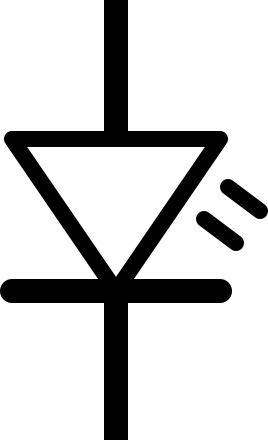
\includegraphics[scale=0.125]{LEDSymbol.png} & LED & An LED is represented by an arrow with a line across it, indicating that current can flow from positive to negative in the direction of the arrow, but it is blocked going the other way.  The LED symbol also has two short lines coming out of it, representing the fact that it emits light. \\
\end{tabular}
\end{center}
\end{figure}

Then, the components are connected together using lines to represent the wires and connections between the components.

Therefore, we can redraw our original circuit using these symbols like you see in Figure~\ref{figCircuitBasicLED}.

\begin{figure}
\caption{Basic LED Circuit Drawn as a Diagram}
\label{figCircuitBasicLED}
\centering
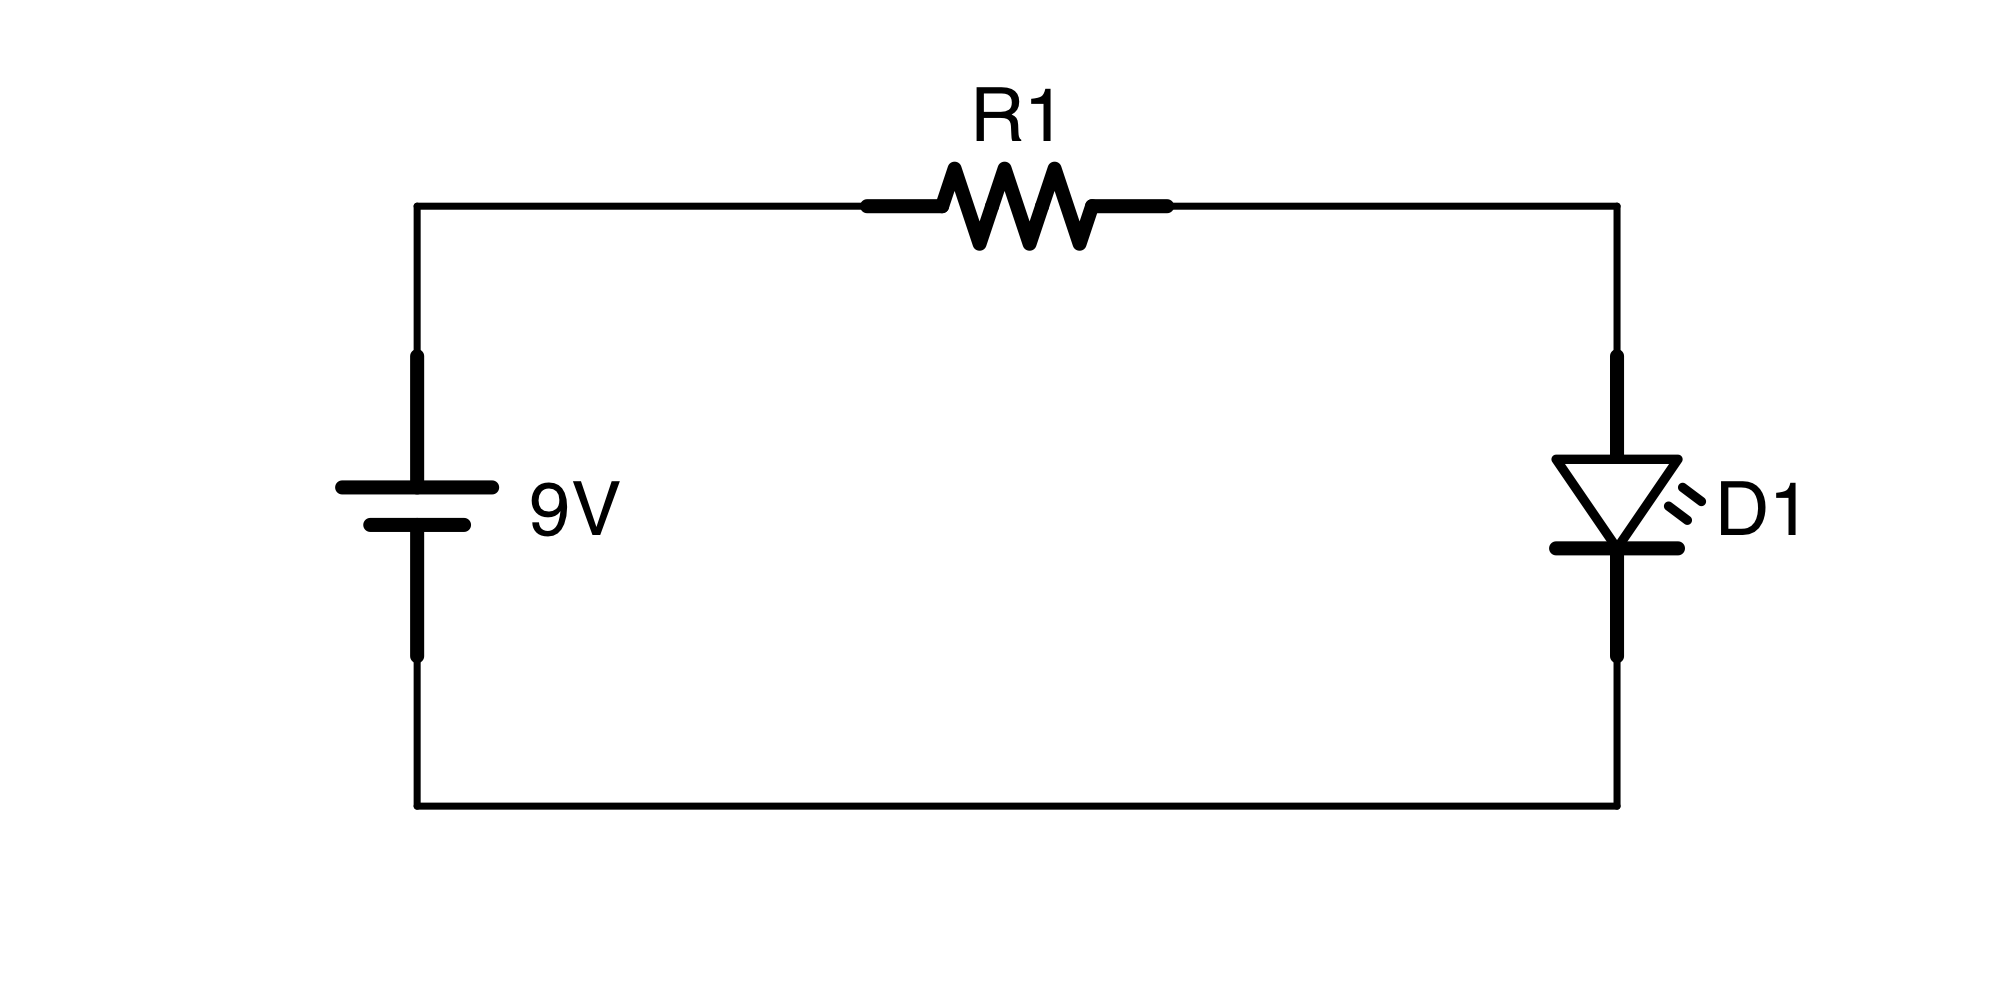
\includegraphics[scale=0.125]{CircuitBasicLED.png}
\end{figure}

Notice that each of our components are laid out on the diagram with wires connecting them.
Remember that it doesn't matter if we have very long wires, very short wires, or if the components are directly placed end-to-end---the resulting circuits will operate identically.
Also notice that each component is labeled (R1 and D1) because, as we make more complicated circuits, it is important to be able to refer back to them.

It does not matter in a diagram which way you have your components turned, how long or short your wires are, or what the general spacing looks like.
When you actually wire it, all of those things will change.
The important part of a circuit diagram is to convey to the reader what the parts are, how they are connected, and what the circuit does in the way that is easiest to read.

For instance, all of the circuits in Figure~\ref{figCircuitLEDAlt} are equivalent to the circuit in Figure~\ref{figCircuitBasicLED}, they are just drawn differently.

\begin{figure}
\caption{Alternative Ways of Drawing the Basic LED Circuit}
\centering
\label{figCircuitLEDAlt}
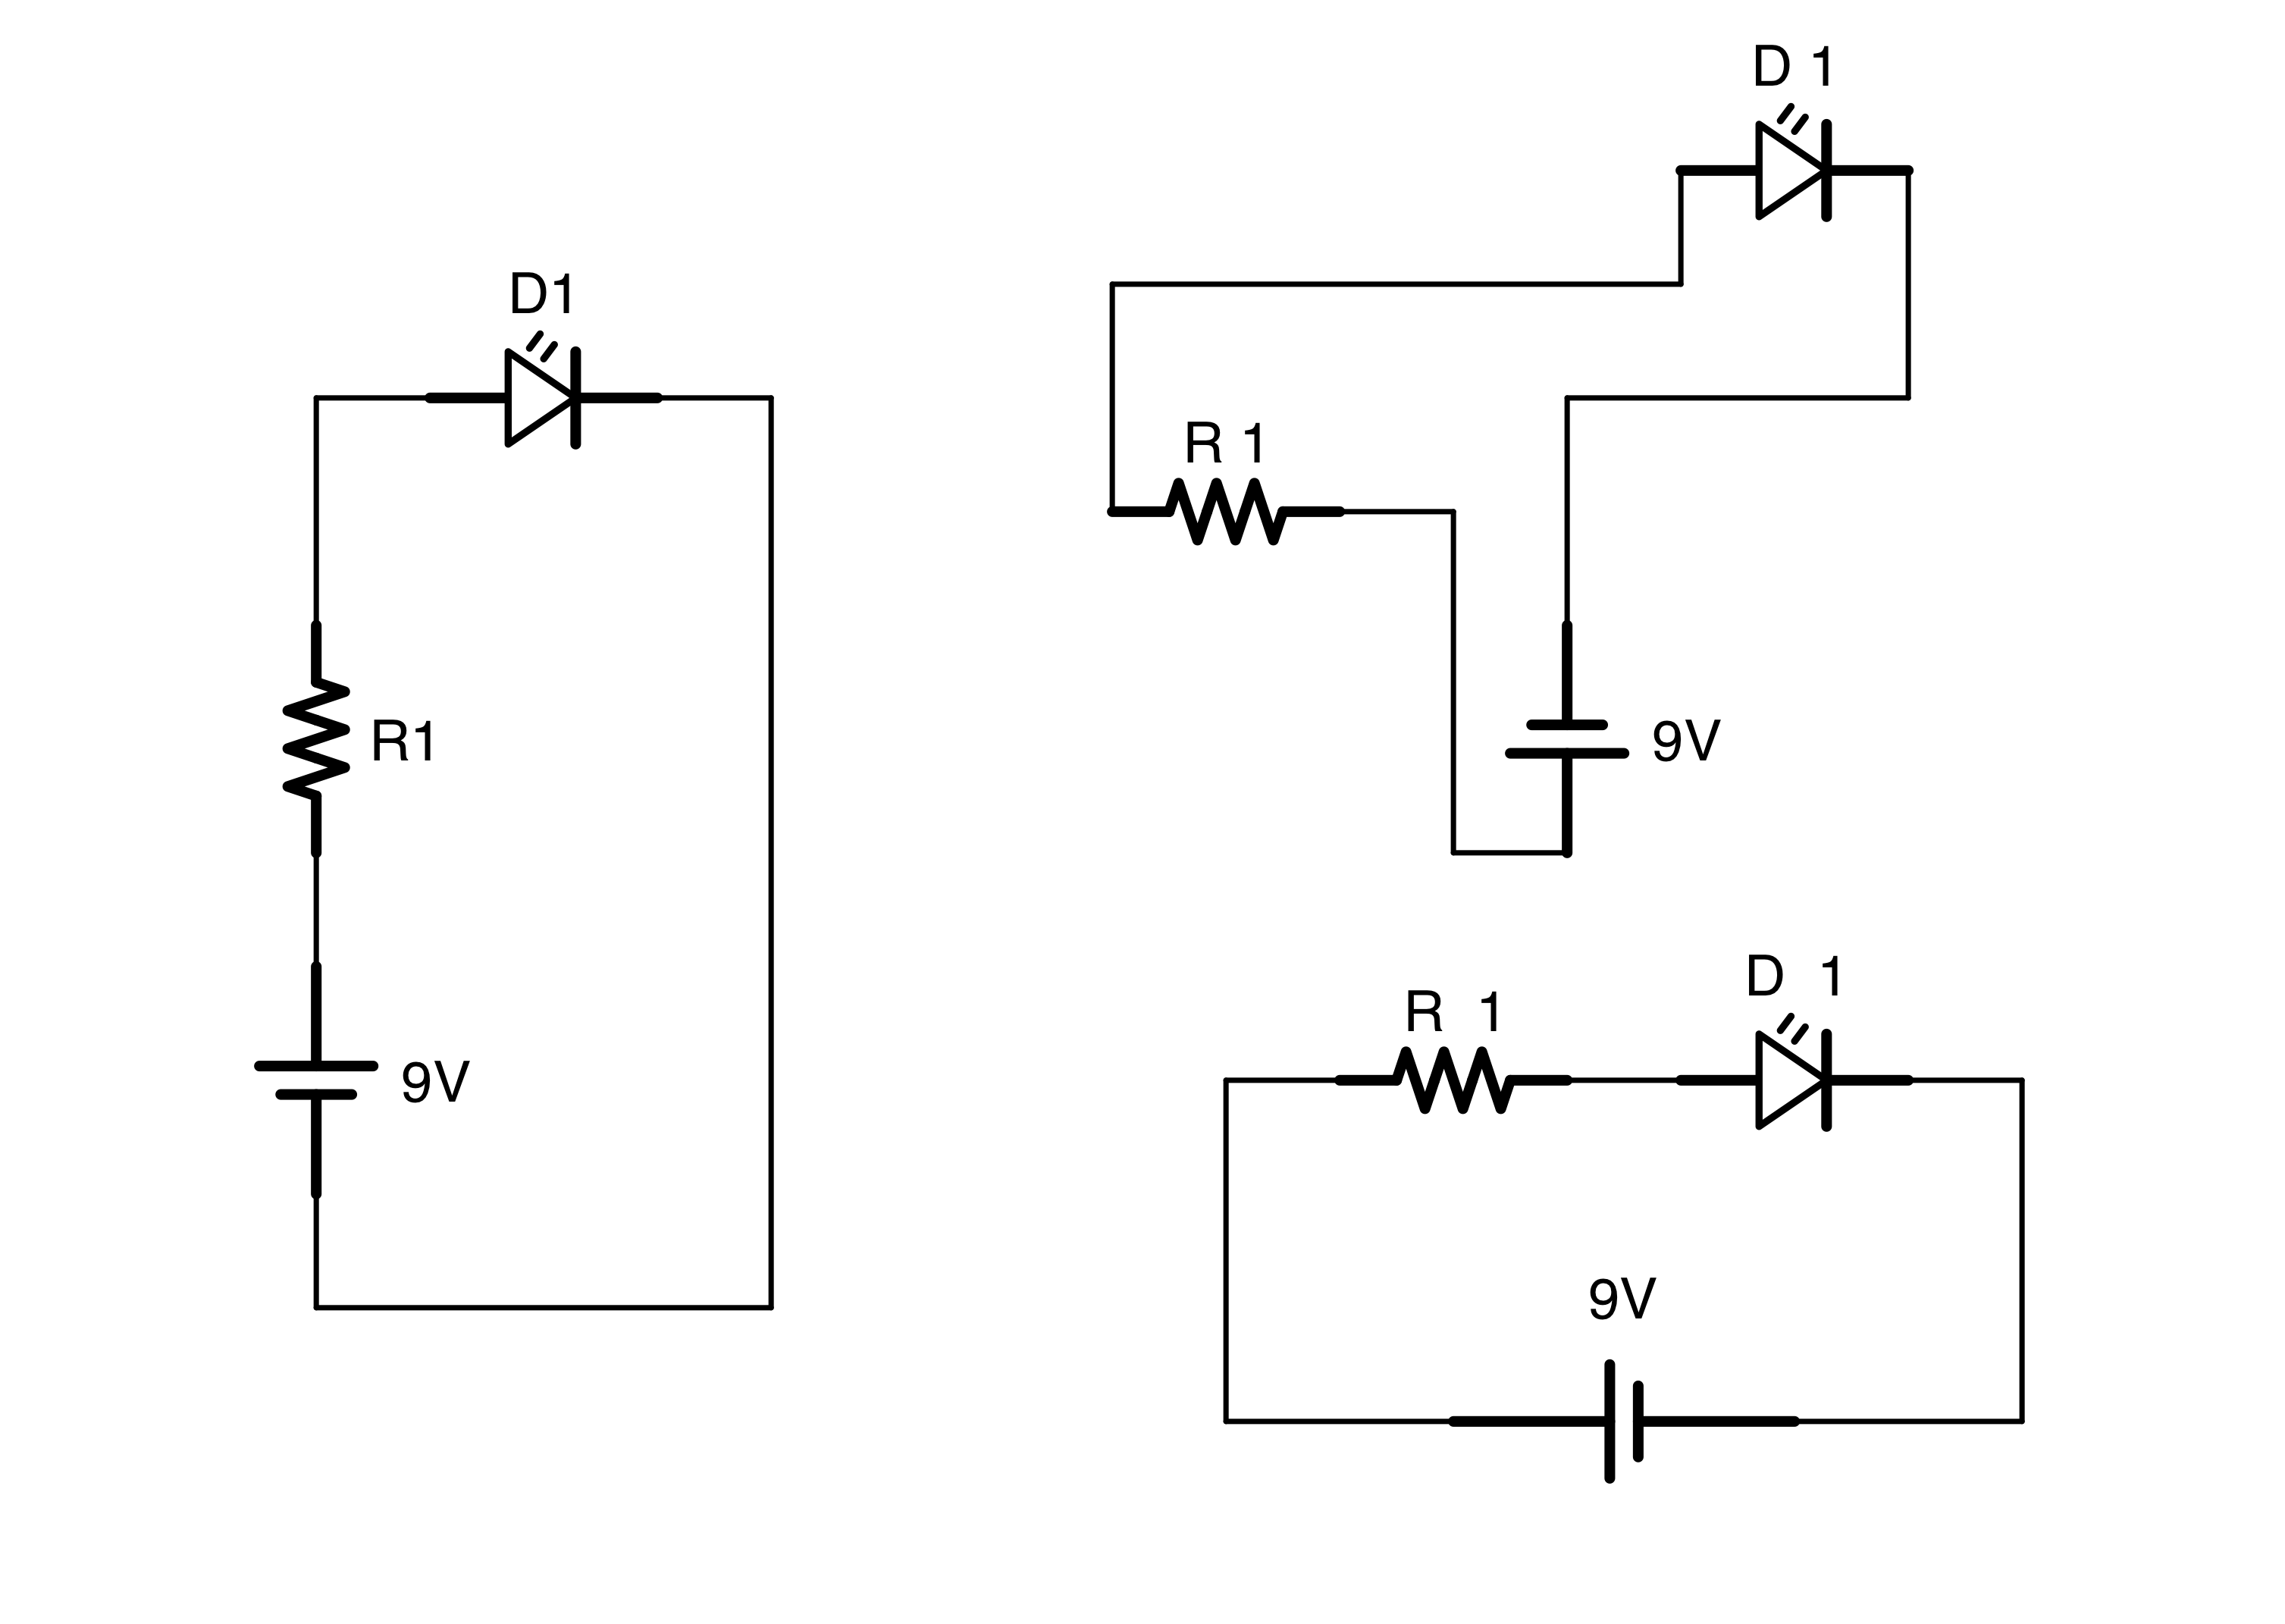
\includegraphics[scale=0.08]{CircuitLEDAlt}
\end{figure}

For consistency, I like to draw all of my batteries to the left of the drawing with the positive side on top.
By keeping the battery positive-side-up, components with higher voltage are usually closer to the top, and components with lower voltages are usually closer to the bottom, with the ground (i.e., zero volts) coming back into the negative terminal.
I also try to make my wire lines as simple as possible in order to make following them easier.

By keeping some amount of consistency, it is easier to look at a drawing and see what it happening.

\section{Drawing the Ground}

Remember that for electricity to move, every circuit must be fully connected from the positive side to the negative side.
That means that in larger circuits there are numerous connections that come from the positive or go back to the ground/negative.
Because of this, a special symbol has been adopted to refer to the ground point in a circuit.
This symbol, the ground symbol, has three lines, each shorter than the next.
Every point on a circuit that has this symbol connected to it is connected to each other (usually they are all connected to the negative side of the battery).

Therefore, the circuit in Figure~\ref{figCircuitBasicLEDGround} is the same circuit as before, just drawn using the ground symbol.
Since every point with the ground symbol are all connected together, using this symbol on both the negative terminal and the negative side of the LED means that they are wired together.

This doesn't help us a lot for this circuit (and, in fact, it makes it a little less easy to read).  
However, in complex circuits, it is much easier to write the ground symbol than trying to have twenty lines drawn back to the negative terminal.

\simplegraphicsfigure{Basic LED Circuit Drawing Using the Ground Symbol}{CircuitBasicLEDGround}{0.08}

Additionally, the same is true with the positive side of the battery.
Many components require a direct connection to a specific voltage to work correctly.
These are usually marked with just a disconnected wire with the end of the wire marking what voltage it requires.
We make less use of that symbol in this book than the ground symbol, but it does come in handy sometimes.

So, using both the voltage source and the ground symbols, we could rewrite the same circuit again in the manner shown in Figure~\ref{figCircuitBasicLEDPosGround}.
This circuit, again, is not \emph{wired} any differently than before.
We are just \emph{drawing} it differently.
For this circuit, it doesn't matter, but in more complex circuits, if we need a specific voltage at a specific location, this symbol tells us to put it there.

\simplegraphicsfigure{Simple LED Circuit Using Positive and Ground Symbols}{CircuitBasicLEDPosGround}{0.08}

\reviewsection

In this chapter, we learned:

\begin{enumerate}
\item Every circuit requires a source of power (usually a battery), wires and components, some amount of resistance, and a complete path back to the negative side of the power source.
\item An open circuit is one that does not connect back to the negative side (and thus does not provide any electricity), and a short circuit is one that connects back to the negative side without any resistance (and thus overwhelms the circuit with current).
\item Batteries supply a fixed voltage between its two terminals.
\item A resistor provides a fixed resistance (measured in ohms) within your circuit.
\item An LED allows current to flow in only one direction, gives off light when current is flowing, but is destroyed when the current goes above 20--30 milliamps.
\item The longer leg of the LED should be on the positive side of the circuit.
\item Wires on a circuit can be almost any length (from zero to a few meters) without changing the functionality of the circuit.
\item A circuit diagram is a way of drawing a circuit so that it is easy to read and understand what the circuit is doing.
\item Each component has its own symbol in a circuit diagram.
\item Every component labeled with the ground symbol is connected together, usually at the negative side of the battery.
\item Voltage sources can be similarly labeled by a wire connected on one side labeled with the voltage that it is supposed to be carrying.
\end{enumerate}

\applysection

\textbf{Special Note} - In the problems below, since we have not yet studied LED operation in-depth, we are ignoring the electrical characteristics of the LED and just focusing on the resistor.  
If you know how to calculate the circuit characteristics using the LED, please ignore it anyway for the purpose of these exercises.

\begin{enumerate}
\item Calculate the amount of current running in the circuit you built in this chapter using Ohm's law.  Since Ohm's law gives the results in amps, convert the value to milliamps.
\item Let's say that the minimum amount of current needed for the LED to be visibly on is 1 milliamp.  What value of resistor would produce this current?
\item Let's say that the maximum amount of current the LED can handle is 30 milliamps.  What value of resistor would produce this current?
\item Draw a circuit diagram of a short circuit.
\item Take the circuit drawing in this chapter, and modify it so that it is an open circuit.
\item Draw a circuit with just a battery and a resistor.  Make up values for both the battery and the resistor and calculate the amount of current flowing through.
\end{enumerate}

\chapter{Constructing and Testing Circuits}
\label{chapConstructingTesting}

%% FIXME - show examples of connected and unconnected wires, and components placed wrongly if I haven't done so already.

In the previous chapter, we learned the theory behind how to analyze circuits.
In this chapter, we are going to put real circuits together and use simple equipment to analyze the same kinds of problems, and compare our calculated answers to the measurements we make on live circuits.

\section{The Solderless Breadboard}

The most important piece of equipment to use for making circuits is the \glossterm{solderless breadboard}.
Before solderless breadboards, if you wanted to put together a circuit, you had to attach them to a physical piece of wood to hold them down, and then \glossterm{solder} the pieces together.
Soldering is a process where two wires are physically joined using heat and a type of metal called solder, which melts at much lower temperatures than other types of metal.
So, what you would have to do is attach the electrical components to the board, wrap the components' legs around each other, and then heat them up with a soldering iron and add solder to join them permanantly.

This was an involved process, and, though it was possible to get your components back, you were generally stuck with your results.
The solderless breadboard is an amazing invention that allows us to quickly and easily create and modify circuits without any trouble at all.
Figure~\ref{figSolderlessBreadboard} shows what a solderless breadboard looks like.

\simplegraphicsfigure{A Solderless Breadboard}{SolderlessBreadboard}{0.5}

The solderless breadboard has a number of spring clips (usually about 400 or 800 of them) called \glossterm{connection points} which will allow you to insert wires or component leads and will hold them in place.
Not only that, the breadboard itself will connect the components for you!

The way that this works is that the breadboard is broken up into little half-rows called \glossterm{terminal strips}.
Each terminal strip has multiple connection points---usually five.
Each connection point on a given terminal strip is connected by wire \emph{inside} the breadboard.
Therefore, to connect two wires or leads together, all you need to do is connect them to the same terminal strip.
Any two wires or leads connected to the same terminal strip are themselves connected.

In most breadboards, the two sides of the breadboard are separated by a gulf known as the \glossterm{bridge}.
The bridge is a visual indication that the two sets of terminal strips are not connected, but it also serves a practical purpose.
If you have an integrated circuit (a small chip), the bridge is the right width so that you can place your integrated circuit right over the bridge, and each leg of the chip will receive its own terminal strip for you to easily connect them to what you need.
We will cover this in more depth in later chapters.

\simplegraphicsfigure{Parts of a Solderless Breadboard}{SolderlessBreadboardParts}{0.5}

In addition to the terminal strips, most breadboards have two strips running down each side, one with a red line and one with a blue line.
These are known as \glossterm{power rails} (some people call them \glossterm{power buses}).  

Power rails are very similar to terminal strips, with a few exceptions.
The main difference is that, in terminal strips, only the five connection points grouped together are connected.
On power rails, many more of the connection points are connected together, even when there are short gaps.
Some boards will split the power rails at the halfway point, but others go all the way down the board.  
This is usually visually indicated by a break in the red and blue lines that indicate the power rails.

Note that the positive and negative are \emph{not} connected to each other (that would create a short circuit), and they are \emph{not} connected to the power rails on the other side of the breadboard (unless you connect them manually).
As we mentioned, on some breadboards, even a single side isn't connected all the way down, but may be broken into sections at the halfway point.

In many projects, many components need direct access to the positive or negative power supply.
Power rails make this easy by providing a connection point with positive and negative power a very short distance away from wherever you need it on the breadboard.
If you plug your power source's positive and negative terminals into the positive and negative rails on the breadboard, then any time you need a connection to the positive or negative terminal, you can just bring a wire to the closest connection point on the appropriate power rail.

\section{Putting a Circuit Onto a Breadboard}

To see how a simple circuit works on a breadboard, let's go back to the circuit we first looked at in Chapter~\ref{chapFirstCircuit}.
Figure~\ref{figCircuitBasicLEDRepeat} has the drawing again for ease of reference.

\begin{figure}
\caption{Basic LED Circuit}
\label{figCircuitBasicLEDRepeat}
\centering
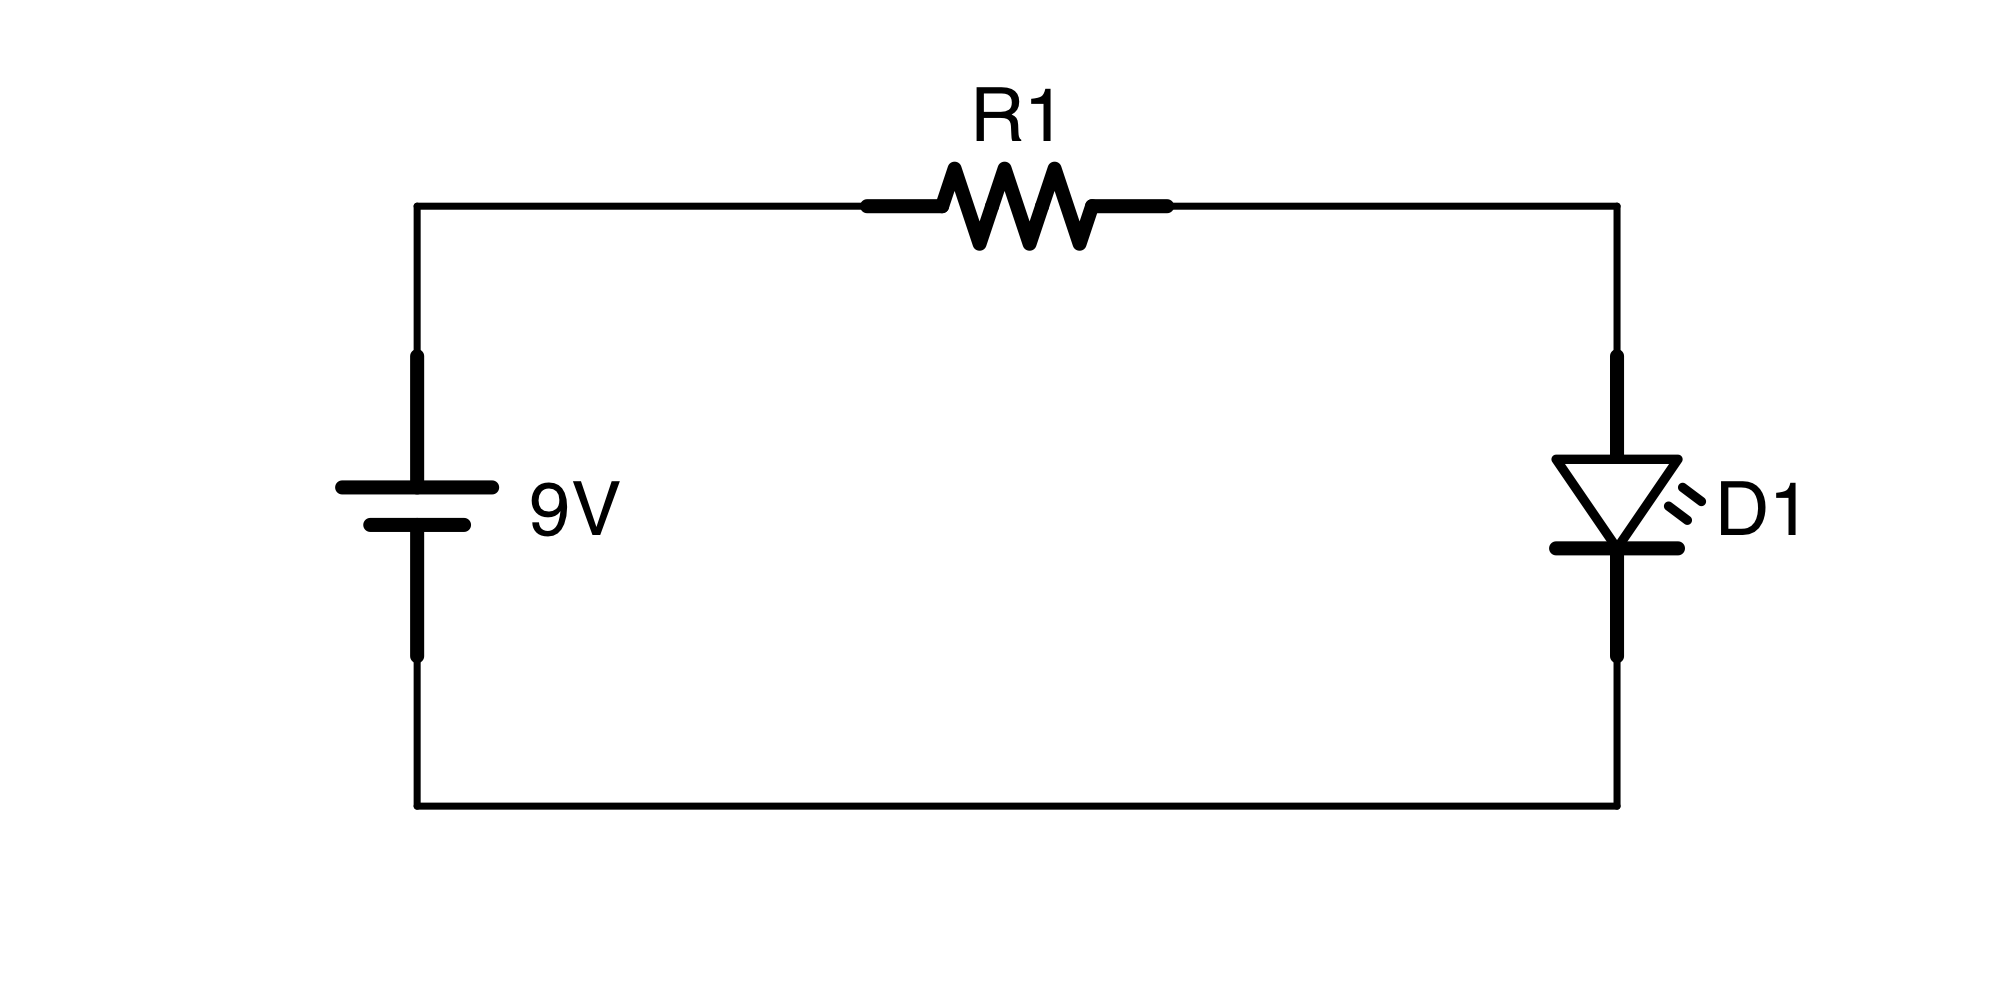
\includegraphics[scale=0.125]{CircuitBasicLED.png}
\end{figure}

So, how do we translate what we see in the drawing to what we need to put in the breadboard?
Well, let's take a look at what is in the circuit---a 9-volt battery, an LED, and a resistor.
Let us not concern ourselves with the battery at the moment.
So, without the battery, we have a resistor connected to an LED.

Let us start out by simply placing our components onto the breadboard.
What you will want is to place them on the breadboard so that each of their legs are on \emph{different} terminal strips.
It doesn't matter \emph{which} terminal strips you use---just make sure the legs all get plugged into different ones.
Figure~\ref{figBreadboardBegin} shows how your breadboard should look so far.
Note that the longer leg of the LED is closer to the resistor.

Figure~\ref{figBreadboardBadEdited} shows the \emph{wrong} way to do it.
In that figure, the both of the legs of the components are on the same row, which is the same thing as placing a wire between the legs, creating a short circuit.
Don't do that!  Make sure each leg goes into its own row.

\simplegraphicsfigure{Putting the Components onto the Breadboard}{BreadboardBegin}{1}

\simplegraphicsfigure{The Wrong Way to Put Components onto the Breadboard}{BreadboardBadEdited}{1}

Now, to connect the resistor to the LED, we need to add a wire.
So, all we need to do is connect a wire to any empty connection point that is on the same terminal strip of the right leg of the resistor, and connect the other side of that wire to the left leg of the LED as shown in Figure~\ref{figBreadboardBeginTwo}.

\simplegraphicsfigure{Adding a Wire to Connect the Components}{BreadboardBeginTwo}{1}

A common mistake that people will make is to connect the wire to the row right before or after the component.
Take some time and be extra certain that the wire is connected to the same row as the leg of your components.

Now, we need to connect our project to the power rails.
So, take a red wire from the left leg of the resistor to the positive power rail (remember, as long as it is in the same terminal strip as the resistor, they will be connected).
Likewise, take a black wire from the right leg of the LED to the negative power rail.
I always use red wires for connecting to the positive power rail, and black wires for connecting to the negative/ground rail, as it makes it more clear when I am looking at my project what wire carries what.
Your project should look like Figure~\ref{figBreadboardBeginThree}.

\simplegraphicsfigure{Adding Wires to the Power Rails}{BreadboardBeginThree}{1}

Now your project is almost done.
All you need to do now is to connect your power rails to a power supply.
Connect a T-connector to a 9-volt battery, and then connect the red (positive) wire to the positive power rail on the breadboard.  You can plug it in anywhere on the rail, but I usually connect the power to the edge of the rail to leave more room for components.
Then, connect the black (negative) wire to the negative power rail on the breadboard.
As soon as you do this, the LED should light up!
Figure~\ref{figBreadboardBeginFour} shows the final circuit.

\simplegraphicsfigure{Final LED Circuit with Power Connected}{BreadboardBeginFour}{1}

Note that many T-connectors for 9-volt batteries have very flimsy wires that are difficult to insert into a breadboard.
Usually, as long as you can get both terminals in far enough to touch the metal within the connection point, it will work.

% FIXME - need more ways of mitigating this problem

If your circuit doesn't work, here is a list of things to check:
\begin{enumerate}
\item Make sure your battery is properly connected to the breadboard---the red should go to positive and the black to negative.
\item Make sure there are \emph{no} wires directly connecting positive to negative on the board.  Any direct pathway from positive to negative without going through a component will cause a short-circuit and can destroy your components and battery.
\item Make sure that your wires are connected to the same terminal strip as the component lead that they are supposed to be connected to.  If they are on a different row, \emph{they are not connected}!
\item Make sure the LED is inserted in the right way.  The longer leg should be connected to the resistor, and the shorter leg should be connected to the negative power supply.
\item Make sure your components are good.  Try replacing your LED with another LED to make sure it works.
\item If all of those things fail, take a picture of your project and post it to the forum mentioned in Chapter~\ref{chapIntro}.  Someone will likely be able to spot your problem and/or lead you in the right direction.  Many other forums are also available on the web for this.
\end{enumerate}

\section{Using Fewer Wires}

In the previous section, we used three wires to connect our components, plus two more wires from the battery.
We can improve our project by reworking it so that most of the wires are not necessary.

Remember that any two leads or wires plugged in next to each on the same terminal strip are connected.
Therefore, we can remove the wire that goes from the LED to the resistor simply by moving the LED and resistor so that the right leg of the resistor is on the same terminal strip.
Figure~\ref{figBreadboardFewerOne} shows what this looks like.

\simplegraphicsfigure{Joining Components by Putting Their Leads on the Same Terminal Strip}{BreadboardFewerOne}{1}

However, that middle wire is not the only redundant wire.  
If you think about it, we could also save a wire by actually using the LED's own leads to go back to the negative rail.
Figure~\ref{figBreadboardFewerTwo} shows how this is setup.
Now, in order to make the LED fit better, it is now on the \emph{other} side of the resistor in the terminal strip.
Remember that this does not matter at all!
No matter where a component is connected on the terminal strip, it is joined with a wire to every other component on the same terminal strip.

\simplegraphicsfigure{Directly Connecting the LED to the Negative Rail}{BreadboardFewerTwo}{1}

Now, there is one last wire that we can get rid of.  
Can you think of which one it is?
If you said the wire going from the positive rail to the resistor---you were right.

What we can do is to directly connect the resistor to the positive rail.
Doing this gives us what is shown in Figure~\ref{figBreadboardFewerThree}.

\simplegraphicsfigure{Connecting the Resistor Directly to the Positive Rail}{BreadboardFewerThree}{1}

Therefore, as you can see, there are any number of ways that you can arrange parts on a breadboard to match a given schematic.  
All of these arrangements we have seen match the schematic given in Figure~\ref{figCircuitBasicLEDRepeat}.
As long as your circuit matches the configuration in the schematic, the specifics of where you put the wires and components is up to you.
Some people like to place the components on their breadboard first, spaced out, and then add wires to connect them as needed.
This works, though it does make for a messier board.
Other people like to use as few wires as possible, and have their layouts as clean as possible (i.e., they don't like a tangled mess).

Some people like to use flexible jumper wires, that goes up and over the board.
Other people like to use rigid jumper wires that lay down close to the board and is the exact length needed.
The flexible wire allows more flexibility in building your circuits (they are easier to move around and reconfigure), while the solid, rigid wire makes the final result a lot cleaner and easier to follow.

You can also trim the legs of your components to make them fit better, if you want.
Some people like to leave their components as intact as possible, while others like to trim the legs of their leads to be the exact right size for their project.
However, if you do trim the leads on your LEDs, be sure to keep the positive leg longer!

However you like to work with electronics is up to you. 
There are lots of options, and they all end up with the same circuit.

\section{Testing Circuits with a Multimeter}

Now that we know how to put circuits together, we need to know how to \emph{test} our circuits.
The main tool used to test simple circuits is the \glossterm{multimeter}.
It is called a multimeter because it measures \emph{multi}ple different things about a circuit.

There are a lot of different multimeters around which have a lot of different functions.
However, almost all of them will measure voltage, current, and resistance.
Each of these values are measured by testing two different points on the circuit.
Most multimeters have a red lead and a black lead.
The red lead should connect to the more positive side of the circuit, and the black lead should connect to the more negative side of the circuit.
However, if you get it reversed, it is usually fine---the multimeter may just report negative values if you are measuring for voltage or current.

\simplegraphicsfigure{A Low-Cost Multimeter}{Multimeter}{0.1}

To illustrate how to use a multimeter, we will start out measuring the voltage in a 9-volt battery.
Remember from Chapter~\ref{chapVoltageResistance} that there is no absolute zero voltage---voltages are merely measured with reference to each other.
Therefore, a multimeter doesn't tell you the exact voltage of something---there is no exact voltage.
Instead, a multimeter allows you to choose two points on your circuit and measure the voltage difference (also known as the \glossterm{voltage drop}) between them.

Now, remember that a 9-volt battery means that the battery should have 9 volts between its positive and negative terminals.
Don't try it yet, but when we measure voltage, we will expect that the multimeter will tell us that the voltage difference is near 9 volts.

When using your multimeter, you must set \emph{what} you are going to test \emph{before} you test it.
Otherwise, you can easily damage your multimeter or your circuit.
Therefore, since we are going to measure voltage, select the DC Voltage setting on your multimeter (\emph{do not} select the DC Current or DC Amperage setting!).
If you are using a high-quality \glossterm{auto-ranging} multimeter, that is all you need to do.
However, when starting out, most people buy the bottom-of-the line multimeter.
That's not a problem, but just know that you will probably accidentally break it at some point.

If you are using a lower-quality multimeter, you will need to not only select \emph{what} you want to measure, but the \emph{estimated range} of values that you want to measure.
On my multimeter, the DC Voltage has five different settings---\icode{1000}, \icode{200}, \icode{20}, \icode{2000m}, and \icode{200m}.
These are the upper boundaries (in volts) that these settings can read (though \icode{2000m} and \icode{200m} indicate millivolts).
Additionally, they indicate the ranges that these settings are best at reading.

So, for a 9-volt battery, using the 1,000-volt setting is probably unwise.
It may give a reading, but it probably won't be accurate.
However, if I try it on too low of a setting (say, 2000m), it either won't read, or it will blow out my multimeter.
So, the safe thing to do is to start with the highest reasonable setting (or just the highest setting if you don't know what's reasonable), test it, and the reduce the setting until it gives you a good reading.

So, for instance, for my 9-volt battery, let's say I didn't know the voltage.
Therefore, I'm going to measure the battery using the 1,000-volt setting.
After setting the multimeter to 1,000 volts, I will put the red lead on the positive terminal of the battery, and the black lead on the negative terminal.
Be sure that you \emph{firmly} press the \emph{tip} of your leads against the positive and negative terminals.  
If it is not firm, or if you use the sides of your terminals, you will not get a good reading.

When I do this, my multimeter reads \icode{9}.  

Now, notice that this reading is significantly less than our 1,000-volt setting.
Therefore, it may not be entirely accurate.  
So, I will reduce the setting to the 200-volt setting and measure again.
This time, my multimeter reads \icode{9.6}.
This is definitely a more accurate reading---it is giving me an extra digit of accuracy!
However, this reading is still significantly below the setting.

Therefore, I will reduce the setting again to the 20-volt setting and re-measure.
This time, the measurement is \icode{9.66}.
Again, it is more accurate.
Now, can I reduce the setting even more?
Well, the next setting is \icode{2000m}, which is basically 2 volts.
Our current reading is 9.66 volts, so it is above the cutoff point for the next setting.
Therefore, I should not try it on a lower setting, both for the sake of accuracy and for the sake of my multimeter's lifespan.

However, I should note that if I did use a lower setting, since the setting is listed as being in millivolts (i.e., \icode{2000m}), then the reading will also be in millivolts.  
That is, if we were to read the value of the battery on that setting, it would say \icode{9660}, because that is how many millivolts the battery has.

Now, you could be wondering, why is a 9-volt battery anything other than exactly 9 volts?
Well, it turns out that in electronics, no value is exact, and no formula works perfectly.
When we talk about a 9-volt battery, we are actually talking about a battery that runs anywhere from 7 volts to 9.7 volts.
In fact, my battery that started out at 9.66 volts will slowly lose voltage as it discharges.
This is one of the reasons why measurement is so important.

Also, this means that in our circuits we will have to find ways to compensate for varying values.
Our circuits should work across a wide range of possible values for our components.
We will discuss strategies for this as we go forward.

The next thing we will measure is resistance.
Pull out a resistor---any resistor.
Appendix~\ref{appendixResistorValues} shows you how to find the resistor values based on the color bands on the resistor.
I don't know about you, but my eyes are not that good at looking at those tiny lines on the resistor and figuring out which color is which.
Many times, it is easier just to test it with the multimeter.

The process is the same as with measuring the voltage.
First, find the resistance settings on your multimeter (perhaps just marked with the symbol for ohms---\si{\ohm}).
Start with the largest value (\icode{2000k}) in my case (\icode{k} means 1,000, so this is a 2,000,000 ohm setting).
On this setting, the multimeter read \icode{000}.
So, I turned it down to the next setting, \icode{200k}.  
This time, it read \icode{00.2}.
So, since the setting is listed in \icode{k} (thousands), this means that the resistor is probably around $0.2\,\si{\kilo\ohm}$, or around $200\,\si{\ohm}$.
However, this is still not an accurate setting.

Next, I turned the dial down to the next setting, which is \icode{20k}.
When I read it this time, it said \icode{0.22}, which would be about $220\,\si{\ohm}$.
Notice how, as the settings on the multimeter get closer to the actual value, I get more and more accuracy.

Next, I turn the dial down to the \icode{1000} setting, since this is still higher than the $220\,\si{\ohm}$ measured so far.
When I read it this time, it says \icode{218}.  
Since the setting does not have a \icode{k} in the name, that means that this reading is $218\,\si{\ohm}$.
On my multimeter, the next setting is \icode{200}, which is less than my last reading, so I will stop and say that my resistor is a $218\,\si{\ohm}$ resistor.

Note that you should \emph{never test for resistance in a live circuit}.
The multimeter uses power to measure resistance, and if there is already power in the circuit, it can damage the multimeter and/or the circuit.

\section{Using a Multimeter with a Breadboard}

We can use our multimeter with our breadboard, too.
Let's say that we wanted to measure the voltage between the positive and negative rails of the breadboard.

There are two ways to do this.
The first, if the size of your multimeter probes and the size of your breadboard connection points allow it, is to simply shove the leads of your multimeter into connection points on the positive and negative rails.
Since these will be connected to the power by a wire, these will be at the same voltage levels as the battery itself.

However, if your breadboard/multimeter combination does not support this, you can do the same thing by simply connecting two jumper wires into the positive and negative rails, and then testing the voltage on the other end of the wires.  

Also, if you are testing components for voltage, you can also use your multimeter on the exposed legs of the component.
This is often easier than either trying to push your leads into the breadboard or running extra wires to your multimeter.

To try out using your multimeter with your breadboard, configure your breadboard similar to Figure~\ref{figBreadboardBeginFour}.  
Use this layout, and \emph{not} one of the ones with fewer wires (you will see why in a minute).
With the battery connected to the breadboard, set your multimeter to the highest voltage setting, and put the red lead in any empty hole in the positive rail.
While that lead is there, put the black lead in any empty hole in the negative rail.

This should give you the same reading that you received for the battery terminals.
Remember that the power rails are connected all the way across---that is why putting your leads in any hole on the line works!
If you work your way down the ranges on your multimeter, you should find that you get the same value that you did when you measured directly on the battery's leads.
Again, if your leads do not fit inside the connection points, you can also use wires to connect out from your breadboard to your multimeter leads.

You can now do the same to any component on your board.
Let's find the voltage difference between one side of the resistor and the other.
To do this, find an empty hole on the same terminal strip as the left-hand side of the resistor, and put the red lead from your multimeter in that hole.
Then, find an empty hole on the same terminal strip as the right-hand side of the resistor, and put the black lead from your multimeter in that hole.
Now you can measure the voltage difference.
Note that to measure voltage differences, the circuit \emph{must} be active.
If the power is gone, the voltage difference will likely drop to zero.
Use the same ranging procedure to find the voltage drop between the left-hand and right-hand side of the resistor.

Even though we have not discussed diodes, this doesn't prevent you from measuring the voltage difference between the legs of the diode in your circuit.
Use the same procedure as before to measure the voltage drop.

\section{Measuring Current with a Multimeter}

Now we will learn to measure current using the same circuit layout from Figure~\ref{figBreadboardBeginFour}.
Like voltage, measuring current requires that the power to your circuit be on.
To measure current, use the DC Amperage (sometimes called DC Current) settings on your multimeter.

Measuring current is a little different than measuring voltage in a circuit.
Instead of just placing your leads in the breadboard as it is, you are going to use your leads to \emph{replace a wire}.
You will remove a wire, and then place your leads in the holes (connection points) where the wire used to be.
Alternatively, if your multimeter does not fit into the connection points, you can again run two wires, one from each hole, from the breadboard to your multimeter leads.

Using either of these approaches, the circuit will then use your multimeter as the wire that was removed, and the multimeter will then measure how much current is running through that wire, and report it to you on the screen.
You will then need to use the same ranging technique as you used before with voltages and resistances to get an accurate report.

Let's say that you wanted to measure the current going through the wire that connects the resistor to the LED.
To do this, we will start by \emph{removing} that wire, and connecting the red lead to where the wire used to be on the left (since it is more positive), and the black lead to where the wire used to be on the right (since it is more negative).
The multimeter should now report back how much current the circuit is using.  
This will vary for a number of reasons, but should be about $17\,\si{\milli\ampere}$.

Now, put the wire back, and remove another wire and measure current there.
No matter which wire you choose, they should all measure the same current.
The reason is that, since all of these components are in series (one right after the other), they must all have the same amount of electricity flowing through them (otherwise, where would the electricity be going?).

\reviewsection

In this chapter, we learned:

\begin{enumerate}
\item Solderless breadboards can be used to quickly create circuits.
\item Solderless breadboards allow circuits to be easily constructed and destructed in such a way that the components are reusable from one project to the next.
\item Both wire and the legs of a component are attached to connection points on the breadboard.
\item Connection points in the same terminal strip are connected by a wire behind the breadboard.
\item To connect two components together, all you have to do is put their legs on the same terminal strip of the breadboard.
\item The power rails on a breadboard extend either all the way down the board, or sometimes split at the halfway point.
\item The bridge of a breadboard divides and separates different groups of terminal strips.  This allows a chip to be placed over the bridge, allowing each of its pins a separate terminal strip.
\item The schematic drawing of a circuit can be assembled onto a breadboard, giving a definite implementation of the drawing.
\item There are multiple different ways to place a given circuit drawing onto a breadboard.
\item Components on a breadboard can be connected by wires, or they can be connected by placing their legs in the same terminal strip.
\item There are many different styles of placing components onto breadboards, which have tradeoffs between how easy it is to reconfigure, and how clean the result is.
\item A multimeter allows you to measure several important values on a circuit, including resistance, voltage, and current.
\item If your multimeter is not auto-ranging, you must test your value several times, starting with the highest range setting for the value you are looking for, and decreasing it through the settings until you find a precise value.
\item Always be sure your multimeter is set to the right setting \emph{before} measuring.
\item Always turn your circuit off before measuring resistance.
\item Your circuit must be on to measure voltage or current.
\item Voltage is measured by connecting your multimeter to empty connection points in the terminal strips that you want to measure.  This can be done either by putting your multimeter leads directly into the relevant connection points or by running wires from those connection points to your multimeter leads.
\item Current is measured by using your multimeter to replace a wire that you want to measure current running through.
\item Many circuit values vary much more than what you might think, so it is good to design circuits in a way that will handle these variances.
\end{enumerate}

\applysection

All measured values should be measured using the ranging technique discussed in this chapter.

\begin{enumerate}
\item Start with the circuit you built in Figure~\ref{figBreadboardBeginFour}.  Measure the voltage drop across the resistor, then measure the voltage drop across the LED.  Now, measure the voltage drop across both of them (put the red multimeter lead on the left side of the resistor and the black multimeter lead on the right side of the LED).  Write down your values.
\item Using the same circuit, change the LED from red to blue.   Measure the values again and write them down.  Measure the current going through the circuit using any wire.  Is it the same or different than before?
\item Add another LED in series with the one you have already.  Measure the voltage drops between each side of each component in the circuit.  Measure the current going through any given wire.  Write down each value.
\item Take the new circuit you built in the previous problem and draw the schematic for the circuit.
\end{enumerate}

\chapter{Analyzing Series and Parallel Circuits}

% FIXME - do I define "voltage drop" anywhere?

In the Chapter~\ref{chapFirstCircuit} we looked at our very first circuit and how to draw it using a circuit diagram.
In this chapter, we are going to look at different ways components can be hooked together and what they mean for your circuit.

\section{Series Circuits}

The circuit built in Chapter~\ref{chapFirstCircuit} is considered a \glossterm{series circuit} because all of the components are connected end-to-end, one after another.
In a series circuit, there is only one pathway for the current to flow, making analyzing the circuit fairly simple.

It does not matter how \emph{many} components are connected together---as long as all of the components are connected one after another, the circuit is considered a series circuit.
Figure~\ref{figSeriesComponents} shows a series circuit with several components included.

\simplegraphicsfigure{A Series Circuit with Several Components}{SeriesComponents}{0.08}

If all of the components are in a series, then even if there are multiple resistors scattered throughout the circuit, you can figure out the total resistance of the circuit just by adding together all of the resistances.
This is known as the \glossterm{equivalent resistance} of the series.

In this example, if R1 is 100\si{\ohm}, R2 is 350\si{\ohm}, and R3 is 225\si{\ohm}, then the total series resistance of the circuit will be $100 + 350 + 225 = 675\,\si{\ohm}$.

That means that the current is easy to figure out as well.
If we ignore the LEDs (since we have not yet learned to calculate using them), then we can use the total series resistance to calculate current the same way we did with the single resistor.

Since the voltage is 9 volts, then we can use Ohm's law to find out the current going through the system.

$$I = V / R = 9 / 675 = 0.013\,\si{\ampere}$$

Note that \si{\ampere} stands for ampere, and we will be using this in our calculations from here on out.
However, in electronics, we usually measure in milliamps (abbreviated as \si{\milli\ampere}), so let us convert:

$$ 0.013 * 1000 = 13\,\si{\milli\ampere}$$

So, our circuit will draw about 13 milliamps of current.
This amount of current is the same amount running through all of the components in the series.

\section{Parallel Circuits}

Circuits are wired into a \glossterm{parallel circuit} if one or more of their components are arranged into multiple branches.

Figure~\ref{figSimpleParallel} shows a simple circuit with two resistors in parallel.
In this figure, the circuit has \emph{two} branches.
R1 is in the first branch, and R2 is in the second branch.
The place where the branch occurs is called a \glossterm{junction}, and is usually marked with a dot to show that all the wires there are connected.

\simplegraphicsfigure{Two Resistors Wired in Parallel}{SimpleParallel}{0.08}

In a parallel circuit, electricity will flow through both branches simultaneously.
Some of the current will go through R1 and some of it will go through R2.
This makes determining the total amount of current more difficult, as we have to take into account more than one branch.

However, there are two additional laws we can use to help us out, known as \glossterm{Kirchoff's circuit laws}.
The guy's name is hard to spell, but his rules are actually fairly easy to understand.

\subsection{Kirchoff's Current Law}

The first law is known as \glossterm{Kirchoff's current law}.
Kirchoff's current law states that, at any junction, the total amount of current going \emph{into} a junction is exactly the same as the total amount of current going \emph{out} of a junction.
This should make sense to us.
Think about traffic at a four-way intersection.
The same number of cars that enter that intersection must be the same number of cars that leave the intersection.
We can't create cars out of thin air, therefore each car leaving must have come in.
Cars don't magically disappear, therefore each car entering must leave at some point.
Therefore, Kirchoff's circuit law says that if you add up all of the traffic going in it will equal the amount going out.

\begin{advsidebar}{Another Way of Looking at It}
Another way to say this is that the total amount of all of the currents at a junction is zero.
That is, if we consider currents coming in to the junction to be positive and currents going out of the junction to be negative, then their total will be zero since the size of the currents coming in must equal the size of the currents going out.
\end{advsidebar}

So, let's look at a junction.
Figure~\ref{figSimpleJunction1} shows a junction where one wire is bringing current in, and it branches with two wires bringing current out.  
The first wire going out has $0.75\,\si{\ampere}$ of current, and the second wire going out has $0.34\,\si{\ampere}$ of current.
How much current is going into the junction from the left?

\simplegraphicsfigure{A Simple Junction}{SimpleJunction1}{0.08}

Since the total coming in must equal the total coming out, then that means the total coming in must be 

$$0.75\,\si{\ampere} + 0.34\,\si{\ampere} = 1.09\,\si{\ampere}$$

Therefore, the total amount of current coming into the circuit is $1.09\,\si{\ampere}$.

Now, lets say we had a junction of four wires.  
In the first wire, we have $0.23\,\si{\ampere}$ of current coming in.
On the second wire, we have $0.15\,\si{\ampere}$ of current going out.
On the third wire, we have $0.20\,\si{ampere}$ of current going out.
What must be happening on the fourth wire?
Is current coming in or going out on that wire?

To figure that out, we have to look at the totals so far.
Coming in, we have the one wire at $0.23\,\si{\ampere}$.
Going out, we have the two wires for a total of $0.15\,\si{\ampere} + 0.20\,\si{\ampere} = 0.35\,\si{\ampere}$.
Since we only have $0.23\,\myamp$ coming in, but there is $0.35\,\myamp$ going out, that means that the fourth wire must be bringing current in.
Therefore, the amount that this fourth wire must be bringing in is $0.35\,\myamp - 0.23\,\myamp = 0.12\,\myamp$.

\subsection{Kirchoff's Voltage Law}

Kirchoff's current law makes a lot of sense, because the amount of ``stuff'' coming in is the same as the amount of ``stuff'' going out.
This is similar to our everyday experience.
Kirchoff's voltage law, however, is a bit more tricky.
\glossterm{Kirchoff's voltage law} states that, given any two points on a circuit at a particular time, that no matter what path is travelled to get between those two points, the difference in voltage between the two points (known as the \glossterm{voltage drop}) is the same \emph{no matter what pathway you take to get there}.

Figures~\ref{figKirchoffVoltageLawExample0}~and~\ref{figKirchoffVoltageLawExampleComposite} illustrates this point.
If we wanted to measure the voltage drop between the two points indicated (A and B), then that voltage drop, at least at a particular point in time, will be the same no matter what pathway electricity travels.
The direct route between the two points has the same voltage drop as the more winding pathways, no matter what the values of the resistors are.

\simplegraphicsfigure{A Circuit With Many Parallel Paths}{KirchoffVoltageLawExample0}{0.08}
\simplegraphicsfigure{All Paths Between Two Points Have the Same Voltage Drop}{KirchoffVoltageLawExampleComposite}{0.05}

So how does that square with Ohm's law?

The way it works is that Ohm's law will cause all of the \emph{currents} through each part of the circuit to adjust in order to make sure that the \emph{voltage} stays the same.

As you can see, the voltage drop between A and B \emph{must} be 9 volts because the battery is a 9-volt battery, and there are no components (only wires) between the battery terminals and A and B.
Since batteries always have a constant voltage between their terminals, that means that A and B will have the same voltage---9 volts.

Therefore, that means that the voltage drop across R1 is 9 volts, because it is one of the pathways between A and B, and all pathways get the same voltage.
Let's put in some real values for these resistors and see if we can figure out how much voltage and current is happening in each part of the circuit.
Let's set R1 = $1,000\,\si{\ohm}$, R2 = $500\,\si{\ohm}$, R3 = $300\,\si{\ohm}$, R4 = $400\,\si{\ohm}$, and R5 = $800\,\si{\ohm}$.
Now, let's find out what our circuit looks like.

As we have noted, \emph{every} path must have the same voltage drop---9 volts.
So let's start with the easiest one, the current going across R1.
Since we have a 9-volt drop and $1,000\,\si{\ohm}$, we can just use Ohm's law for current: 

$$I = V / R = 9\,\si{\volt} / 1,000\,\si{\ohm} = 0.009\,\myamp$$

So, we have $0.009\,\myamp$ running across R1.

Now, what about R2?
R2 is connected to point A simply by a wire.
As we mentioned in Section~\ref{secWireRule}, wires can be considered to be zero-length.
Therefore, R2 is just as much directly connected to point A as R1 is.
Therefore, the voltage drop across R2 is also going to be 9-volts.
Again, using Ohm's law, we can see that 

$$I = V / R = 9\,\si{\volt} / 500\,\si{\ohm} = 0.018\,\myamp$$

So, the current going across R2 is $0.018\,\myamp$.

What about the current going across R3, R4, and R5?
Well, if you notice, those resistors are all in series, so we can add them all up and just use the total resistance.

So, the total resistance for this section of the circuit will be:

$$R3 + R4 + R5 = 300\,\si{\ohm} + 400\,\si{\ohm} + 800\,\si{\ohm} = 1,500\,\si{\ohm}$$

So, using Ohm's law, the current running through this part of the circuit will be:

$$I = V / R = 9\,\si{\volt} / 1,500\,\si{\ohm} = 0.006\,\myamp$$

Now, remember that the total current flowing into any junction has to be equal to the current flowing out of it.
So, let's look at the junction between R2 and R3.  
We calculated that the current flowing to R2 is $0.018\,\myamp$ and the current flowing to the series starting with R3 is $0.006\,\myamp$.
Therefore, there has to be $0.018 + 0.006 = 0.024\,\myamp$ flowing into that junction.

Now, how much current is flowing out of junction A?
Well, earlier, we noted that the amount of current flowing across R1 was $0.009\,\myamp$, and we just calculated that there is $0.024\,\myamp$ flowing out of A into the junction between R2 and R3. 
That means that there must be $0.033\,\myamp$ total flowing into junction A.

While there were a lot of steps to determine this, each individual step was fairly straightforward.
We simply combined Ohm's law, Kirchoff's voltage law, and Kirchoff's current law to figure out each step.

Now, one important thing to notice is that there is \emph{less} current running through the pieces of the circuit with more resistance than there is with the pieces of the circuit with less resistance.
The electric current is more likely to go down the path of least resistance.
This is a very important point and should not be overlooked, as it will come in handy in later chapters.

\section{Equivalent Parallel Resistance}

The sort of calculation that we have done in the previous section gets trickier if there is a series resistance before or after the parallel resistance.
Figure~\ref{figKirchoffVoltageLawSeriesAndParallel} gives an example of this.
The setup is just like the previous circuit, except there is a single resistor (R6) in series with the battery \emph{before} the parallel branches.
This will prevent our simple calculations from working because the current flowing in each of the branches of the circuit will all add together to tell us the amount of current flowing through R6.
However, the voltage drop across R6 will depend on the current flowing through it.
If this voltage changes, then it will change our starting voltage for our calculations to figure out the parallel branches.

\simplegraphicsfigure{Kirchoff's Voltage Law with Series and Parallel Components}{KirchoffVoltageLawSeriesAndParallel}{0.08}

Thus, we have ourselves in a loop---in order to find out the current flowing through the parallel branches, we have to know their starting voltage.
In order to find out their starting voltage, we have to know how much the voltage dropped across R6.
In order to know how much the voltage dropped across R6, we have to know how much current was flowing through it!

This may seem like an impossible problem, but basic algebra allows us to work it out, though the details are kind of ugly.
Instead, we have an equation which gives us \glossterm{equivalent resistance}.
That is, we can take a series of parallel resistors, and we can calculate the total resistance of those resistors.

If you have resistors in parallel to each other (let's call them $R_1$, $R_2$, and $R_3$), and you want to know the resistance of their \emph{combined} action (which we will call this total $R_T$), then you would use the following equation:

\begin{equation}
\label{eqparallelresistancethree}
R_T = \frac{1}{\frac{1}{R_1} + \frac{1}{R_2} + \frac{1}{R_3}}
\end{equation}

This equation works for any number of resistances that we have in parallel.
We can just keep on adding them to the end of the list:

\begin{equation}
\label{eqparallelresistancen}
R_T = \frac{1}{\frac{1}{R_1} + \frac{1}{R_2} + \ldots + \frac{1}{R_N}}
\end{equation}

So, let's look at our circuit, and see how we can find out the currents flowing through each resistor.
For this example, we will again say that $R1 = 1,000\,\si{\ohm}$, $R2 = 500\,\si{\ohm}$, $R3 = 300\,\si{\ohm}$, $R4 = 400\,\si{\ohm}$, and $R5 = 800\,\si{\ohm}$.  Additionally, $R6 = 250\,\si{\ohm}$.

In order to compute this, we first have to figure out \emph{what} is in series and what is in parallel.
Notice the loop made by R3, R4, and R5.  
Those are all connected end-to-end, so they are in series.
Because they are in series, we can get their equivalent resistance just by adding them together---$300 + 400 + 800 = 1,500\,\si{\ohm}$.
Therefore, we can actually \emph{replace} these resistors with a single, $1,500\,\si{\ohm}$ resistor.
We will call this ``combined'' resistor R7.
Now, if you look at the new picture, with R7 standing in for the loop, you will see that R1, R2, and R7 are in parallel with each other.

Therefore, we can find out their combined resistance by using Equation~\ref{eqparallelresistancen}:

\begin{align*}
R_T &= \frac{1}{\frac{1}{R1} + \frac{1}{R2} + \frac{1}{R7}} \\
R_T &= \frac{1}{\frac{1}{1,000} + \frac{1}{500} + \frac{1}{1,500}} \\
R_T &= \frac{1}{0.001 + 0.002 + 0.00067} \\
R_T &= \frac{1}{0.00367} \\
R_T &= 272.5\,\si{\ohm}
\end{align*}

Therefore, the equivalent resistance of all of the parallel resistances is about $272.5\,\si{\ohm}$, which means that we can replace \emph{all} of these resistors (R1, R2, R3, R4, and R5) with a single resistor that is $272.5\,\si{\ohm}$.
Also notice that this resistance is actually \emph{less} than each of the individual resistances.

Now, to get the total resistance of the circuit, we notice that this parallel resistance ($272.5\,\si{\ohm}$) is in series with R6, which is $250\,\si{\ohm}$.  
Since they are in series with each other, we can simply add them together.
The total resistance of this circuit is $250 + 272.5 = 522.5\,\si{\ohm}$.
We can now use Ohm's law to find the total amount of current running through this circuit:

\begin{align*}
I &= \frac{V}{R} \\
I &= \frac{9}{522.5} \\
I &= 0.0172\myamp
\end{align*}

Thus, the whole circuit has 0.0172 amperes of current running through it.
Using this, we can now go back through and identify how much current and voltage is flowing through each individual piece.

Because the entirety of the 0.0172 amperes is going through the first resistor, that means that the voltage drop of this resistor will be, using Ohm's law:

\begin{align*}
V &= I\cdot R \\
V &= 0.0172 \cdot 250 \\
V &= 4.3\,\si{\volt}
\end{align*}

That means that this resistor will chew up $4.3\,\si{\volt}$.  
This leaves us with $9 - 4.3 = 4.7\,\si{\volt}$ left after the series resistor.

We now know the starting and ending voltages of each branch of the parallel resistors---$4.7\,\si{\volt}$ at the beginning (what we just calculated the voltage to be after the series resistor), and $0\,\si{\volt}$ at the end (because it connects to the negative terminal of the battery, which we have designated as the zero volt reference).

Therefore, we can use Ohm's law to find the amount of current flowing through each of them.
For R1:

\begin{align*}
I &= \frac{V}{R} \\
I &= \frac{4.7}{1,000} \\
I &= 0.0047\,\si{\ampere}
\end{align*}

For R2:

\begin{align*}
I &= \frac{V}{R} \\
I &= \frac{4.7}{500} \\
I &= 0.0094\,\si{\ampere}
\end{align*}

And finally, for the series that is in a loop at the right (R3, R4, and R5):

\begin{align*}
I &= \frac{V}{R} \\
I &= \frac{4.7}{1500} \\
I &= 0.0031\,\si{\ampere}
\end{align*}

Since the loop is all in series, that means all of the resistors in that series will have $0.0031\,\si{\ampere}$ going through them.

If we add all of these currents, we will see that $0.0031 + 0.0094 + 0.0047 = 0.0172\,\si{\ampere}$, which is the amount of current we originally figured out.

What we have learned is that we can replace the entire circuit with a single value for its resistance to figure out how the circuit will behave as a whole.
For a simple circuit like this, having all of these parallel branches doesn't do much, so it may seem pointless.
However, in a real circuit, each of these branches may be, instead of a resistor, a component that has some amount of resistance.
If you know the resistance, you can calculate how much current is flowing through it the same way.

However, we start with only resistors in order to make the problems simpler.

% FIXME - put this somewhere after we talk about LEDs/diodes more in-depth.  A corollary to that law is that if the calculated voltage drop between two components down a particular pathway must be more than another voltage drop by a different pathway, the pathway with the larger voltage drop can be considered to be disconnected.

\section{Wires in a Circuit}

In complicated circuits, sometimes we run out of room and must draw wires on top of each other even though the wires aren't connected.
In this book, we try to make clear which wires are connected by placing a dot on the junction point.
To show two wires that don't connect to each other, but which had to cross because the diagram was too complicated to prevent it, we will show one of the wires as being broken across the intersection point.
Figure~\ref{figJoinedVsUnjoinedEdited} demonstrates the difference.
The wires on the left are joined together as indicated by the dot.
The wires on the right are not joined in any way, they just had to be drawn across each other because of space reasons in the diagram.

\simplegraphicsfigure{Joined Wires (left) vs. Unjoined Wires (right)}{JoinedVsUnjoinedEdited}{0.08}

Also, the lengths of wires that we draw are irrelevant.  
Usually, in simple circuits, we should consider that wires are all zero-length.
If, after a resistor, the voltage in the circuit has dropped to $5\myvolt$, then we can consider that the \emph{whole wire} until the next circuit is at $5\myvolt$.  
If a wire branches into multiple branches, even though each branch will have a different amount of \emph{current} running on the branch, each branch of the wire will all have the \emph{exact same voltage} until they reach another component.

Therefore, in the circuit in Figure~\ref{figEquivalentPoints}, you can see several points labelled A, B, C, D, E, F, and G.
In this circuit, A, B, and C all have equivalent voltages (though not equivalent currents) since there are only wires (and not components) between them.
Likewise, D, E, F, and G all have equivalent voltages since there are only wires between them.  
Also, since D, E, F, and G are all connected to the battery negative (i.e., ground) with no components between them, that means that they are all at zero volts.
Likewise, since A, B, and C are all directly connected to the battery positive with no intervening components, they are all at 9 volts.

\simplegraphicsfigure{Several Points on a Circuit}{EquivalentPoints}{0.08}

\reviewsection

In this chapter, we learned:
\begin{enumerate}
\item In a series circuit, electricity flows in a single line through all of the components.
\item In a parallel circuit, electricity branches and flows in multiple branches.
\item Most real circuits are combinations of series and parallel circuits.
\item When you have resistors together in series, the total resistance of all of the resistors combined is simply the sum of their individual resistances.
\item In a parallel circuit, Kirchoff's Current Law says that the total amount of current entering a branch/junction is the same as the total amount of current leaving the branch.
\item In a parallel circuit, Kirchoff's Voltage Law says that, between any two points on a circuit at a given point in time, the voltage difference between those two points will be identical no matter what pathway the electricity follows to get there.
\item When resistances are in parallel, the total resistance for the parallel circuit is given by the equation $R_T = \frac{1}{\frac{1}{R_1} + \frac{1}{R_2} + \ldots + \frac{1}{R_N}}$.
\item By using these laws in combination, we can predict how current will flow in each part of our circuit.
\end{enumerate}

\applysection

\begin{enumerate}
\item There is a junction in a circuit that has one wire with current flowing in and two wires with current flowing out.  There is $1.25\myamp$ of current coming in, and the first wire going out has $0.15\myamp$ of current going out.  How much current is leaving through the second wire?
\item There is a junction in a circuit that has two wires with current flowing in and two wires with current flowing out.  The first wire with current flowing in has $0.35\myamp$ of current, the first wire with current flowing out has $0.25\myamp$ of current, and the second wire with current flowing out has $0.42\myamp$ of current.  How much current is flowing in on the second incoming wire?
\item At a junction of four wires, wire 1 has $0.1\myamp$ of current flowing in, wire 2 has $0.2\myamp$ of current flowing in, and wire 3 has $0.4\myamp$ of current flowing out.  Is the current in wire 4 going in or out?  How much current is flowing on it?
\item If I have three $100\myohm$ resistors in series, what is the total resistance of the series?
\item If I have a $10\myohm$ resistor, a $30\myohm$ resistor, and a $65\myohm$ resistor in series, what is the total resistance of the series?
\item If I have a $5\myohm$ resistor and a $7\myohm$ resistor in series, what is the total resistance of the series?
\item If I have two resistors in parallel, a $30\myohm$ resistor and a $40\myohm$ resistor, what is the total resistance of this circuit?
\item If I have three resistors in parallel---$25\myohm$, $40\myohm$, and $75\myohm$, what is the total resistance of this circuit?
\item If I have four resistors in parallel---$1,000\myohm$, $800\myohm$, $2,000\myohm$, and $5,000\myohm$, what is the total resistance of this circuit?
\item If I have three resistors in parallel---$100\myohm$, $5,000\myohm$, and $10,000\myohm$---what is the total resistance of this circuit?  Which of the resistors is the total resistance most similar to?
\item Take a look at the following circuit diagram.  If the voltage drop between B and C is 2 volts, and the voltage drop between C and D is 3 volts, what is the voltage drop between A and E?  What is the voltage at E?  What is the voltage at A? \\ 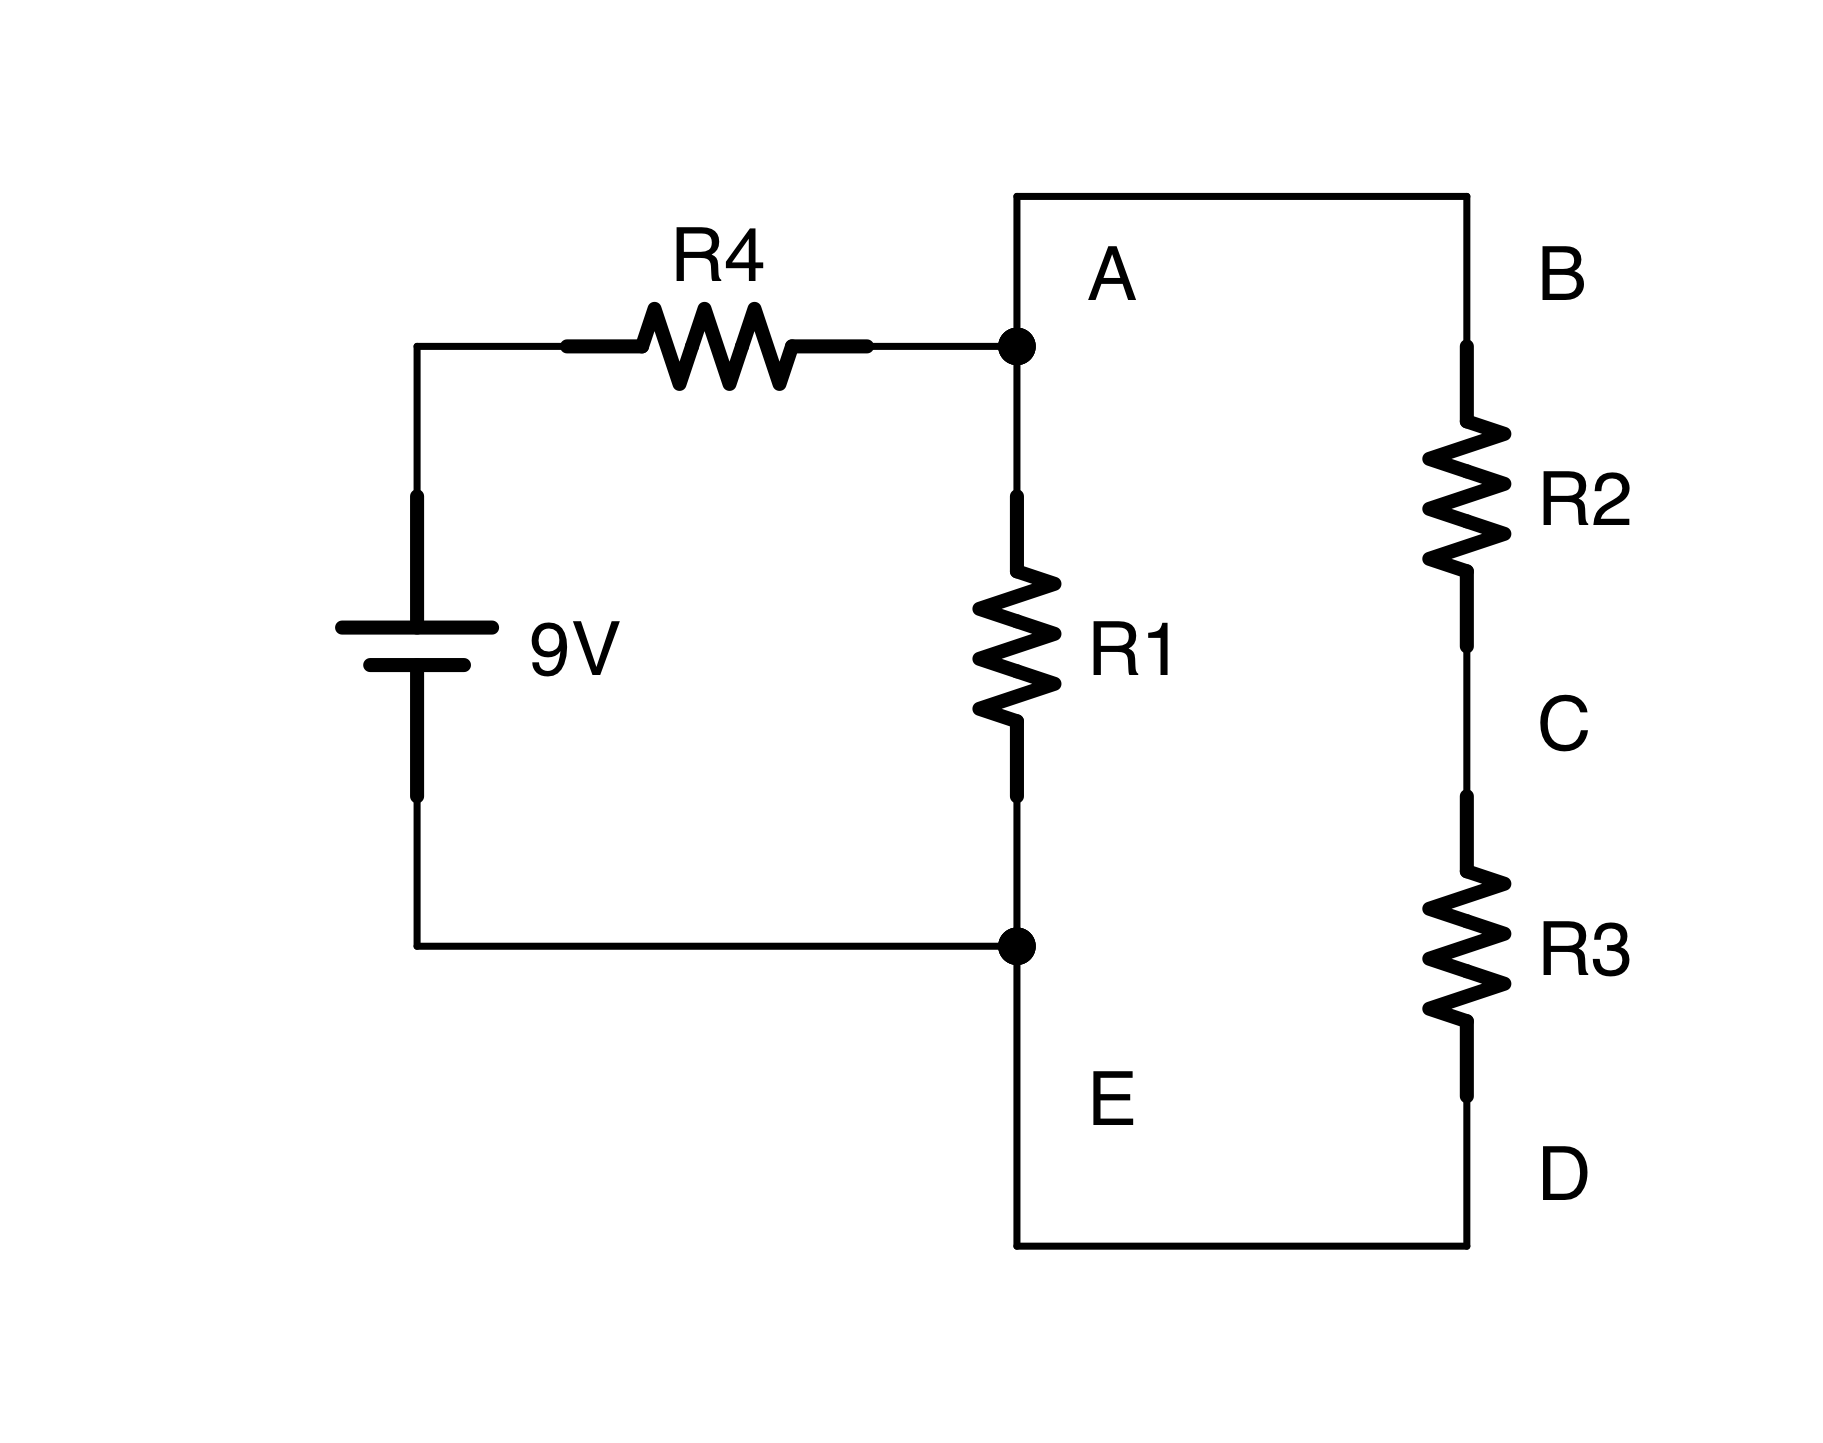
\includegraphics[scale=0.08]{VoltageDropProblem.png}
\item Optional - what resistor values would you need to have the circuit above run with $2\myamp$ total current?
\item The circuit below is a combination of series and parallel resistances.  Each resistor is labelled with its resistance value, given in ohms.  Find out how much current is flowing through each resistor, and how much each resistor drops the voltage.  \\ 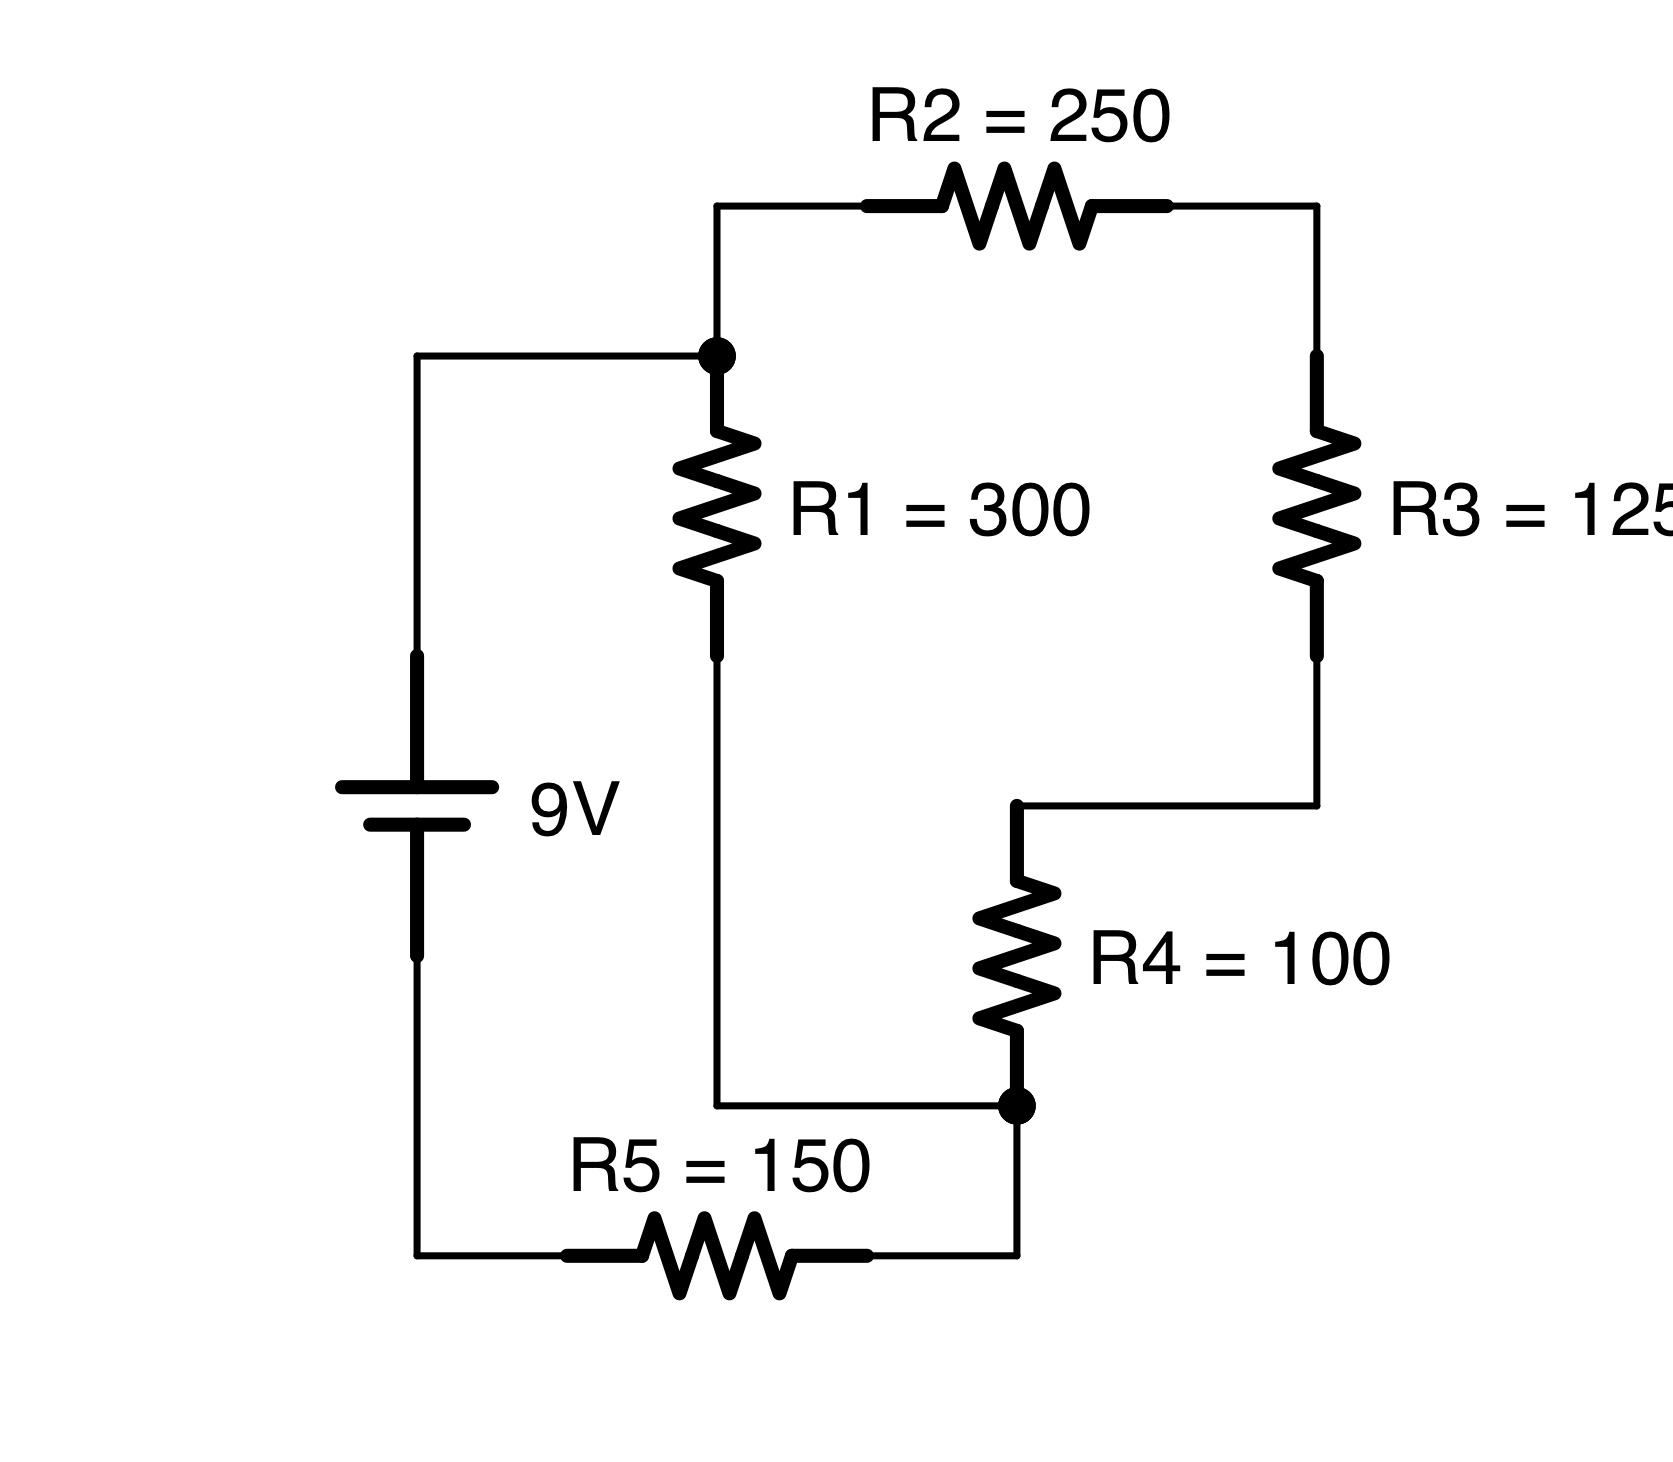
\includegraphics[scale=0.08]{ProblemCalculateCurrentAndVoltage}
\end{enumerate}

\chapter{Diodes and How to Use Them}
label{chapDiodes}

This chapter introduces the \glossterm{diode}.  
We have used light-emitting diodes (LEDs) in previous chapters, but have not really discussed their function except for emitting light.
In this chapter, we are going to look at regular diodes, light-emitting diodes, and Zener diodes, to get a feel for what these devices are and how they might be used in circuits for more than just light.

% FIXME - schematic of a diode

\section{Basic Diode Behavior}

Unlike resistors, diodes have both a positive and negative side.
For any component with both positive and negative legs, the positive leg of the component is termed the \glossterm{anode} and the negative leg is termed the \glossterm{cathode}.
On LEDs, the anode is longer than the cathode.
However, for other types of diodes, the cathode is marked with a line.
You can remember this because in the schematic of a diode, the cathode has the blocking line.

The diode performs two fundamental ``actions'' with electric current.  
The first action of a diode is to drop voltage by an essentially fixed amount \emph{without} affecting or limiting current.
This amount of voltage is called the \glossterm{forward voltage drop} and it is usually around $0.6\myvolt$ for more non-LED diodes. 
Forward voltage is often abbreviated as $\myvolt_F$.
For most LEDs, the forward voltage drop depends on the color of the LED, with a red LED dropping about $1.8\myvolt$ and a blue LED dropping about $3.3\myvolt$.
The forward voltage drop can vary among the other colors as well.

To remind you, when we say ``voltage drop,'' we are referrig to the difference in voltage between the positive and negative leg of the diode.
Therefore, no matter what the voltage is coming into the diode, the voltage coming out of the diode will be that voltage minus the voltage drop.

The second action of a diode is to limit the direction of current to a single direction.
With some exception, the diode only allows current to flow one way in the circuit.
The ``normal flow'' of a current through the diode is to flow from the anode to the cathode.
Looking at the schematic symbol, current flows in the direction that the arrow is pointing, and current is blocked from flowing the other way (you can think of the line as a ``block'' preventing reverse flow).

However, diodes are limited in the amount of reverse flow they can block.
At a certain point, diodes reach their \glossterm{breakdown voltage}.
The breakdown voltage is the voltage at which they will stop blocking voltage.
In regular diodes, this is a failure mode and the precise value shouldn't be relied upon (we will see an exception to this with Zener diodes). %% FIXME - refer to specific section on Zener diodes
Usually, though, this value is high enough not to worry about (i.e., around 100 volts).

\section{Circuit Calculations with Diodes in Series}

Now let's talk about how to properly calculate the behavior of circuits with diodes.
Remember, the key to a diode is that if current is flowing through the diode, the voltage drop across the diode will be essentially constant.
For a normal non-LED diode, this voltage drop is almost always $0.6\myvolt$.
This is so common it is usually assumed, and never listed in the circuit itself.

Therefore, take a look at the circuit in Figure~\ref{figDiodeWithResistor}.
Since the voltage source is 9 volts, that means that the total voltage drop between the positive and negative is 9 volts.
The diode will eat $0.6\myvolt$ of the voltage, but will not limit the current in any way.
The resistor, then, since it is the only component left, will use up the rest of the voltage---$8.4\myvolt$.
Therefore, we can calculate the current in the circuit using Ohm's law:

$$I = V / R = 8.4 / 1000 = 0.0084\myamp = 8.4\mymamp$$

\simplegraphicsfigure{A Diode and Single Resistor Circuit}{DiodeWithResistor}{0.08}

Therefore, our circuit will use $8.4\mymamp$ of current.
So, as you can see, when doing calculations, the diodes simply provide a drop in voltage, they do not limit current.

This is true no matter how many diodes or resistors I have in my circuit.
Figure~\ref{figMultipleDiodesResistors} shows a circuit like that.
To figure out the behavior of this circuit, remember that \emph{every} diode has a $0.6\myvolt$ voltage drop.  Since the circuit has three diodes, that means that the diodes will drop a total of $0.6 * 3 = 1.8\myvolt$.

Therefore, we will have $1.8\myvolt$ taken up by diodes, which drop voltage without limiting current.  
Since we have a $9\myvolt$ source, there will be $9 - 1.8 = 7.2\myvolt$ that is not eaten by diodes.
This voltage will go to our two resistors.  
These resistors, even though they are separated by diodes, are essentially in series with each other.
Therefore, we can treat them as a single resistor in series.
So, the total resistance on the circuit will be $1k + 2k = 3k\myohm$.

We can then find the total current running through the circuit using Ohm's Law:

$$ I = V / R = 7.2\myvolt / 3,000\myohm = 0.0024\myamp = 2.4\mymamp$$

\simplegraphicsfigure{A Circuit with Multiple Diodes and Resistors}{MultipleDiodesResistors}{0.08}

However, it is possible to put too many diodes in your circuit.
Since they each eat $0.6\myvolt$ in their forward voltage drop, that puts a limit on how many you can string together in series from a given battery.
For a $9\myvolt$ battery, if I try to put 20 diodes together in series, I will have used \emph{more} than the total 9 volts that I have available.  
Therefore, current will not flow.
With 20 diodes, the voltage drop will be $20 * 0.6 = 12\myvolt$.  
Since this is more voltage than the battery can put out, no current will flow.

So, we have seen two conditions for which current will not flow through a diode---the first is that the diode will block current from flowing in the wrong direction, and the second is that the diode will not conduct if the voltage source cannot provide enough voltage to bridge the forward voltage drop of the diode.

\section{Circuit Calculations with Diodes in Parallel}

The real magic of diodes comes when using them in parallel circuits.
Remember the rules that we learned in Chapter~\ref{chSeriesParallel}.
Kirchoff's Voltage Law says that between any two points, the voltage drop between those two points will be the same \emph{no matter what path the current follows}.
Therefore, since the voltage drop across a diode is \emph{fixed}, that means that we can guarantee a maximum voltage drop between two points on a circuit by putting diodes between them.

\simplegraphicsfigure{A Single Diode in Parallel with a Resistor}{ParallelDiode}{0.08}

Figure~\ref{figParallelDiode} shows what this looks like.  
The voltage drop from one side of the diode to the other is $0.6\myvolt$.
Period. End of story (actually, it could be less, which would keep the diode from conducting altogether, but we won't consider that at the moment).

Kirchoff's Voltage Law tells us that \emph{no matter what path is travelled}, the voltage difference between those two points will be the same.
Since the 2k resitor is attached to the same two points that the diodes are attached to, Kirchoff's Voltage Law tells us that the voltage across the resistor \emph{must} be the same as the voltage across the diode.
Thus, the voltage across the resistor \emph{must} be $0.6\myvolt$.

Using Ohm's law, we can deduce the amount of current flowing through that resistor:

$$ I = V / R = 0.6 / 2,000 = 0.0003\myamp = 0.3\mymamp $$

So how much current is flowing through the diode?
To find this out, we need to use Kirchoff's Current Law.
The amount entering the junction where the diode and the 2k resistor splits off is the same as the amount leaving it.
We know that $0.3\mymamp$ leaves the junction to go to the resistor.
Therefore, if we could figure out how much current was coming \emph{into} the junction we could figure out how much is going through the diode.

To discover that value, we need to know how much current is going through the 1k resistor.
To figure that out, we need to know the voltage drop across the resistor.
However, we can figure this out easily.  
Since the tail end of the diode is connected to ground (the negative terminal), that means that after the diode we are at $0\myvolt$.  
Therefore, since the diode voltage drop is $0.6\myvolt$, then the voltage before the diode must be $0.6\myvolt$.
That means that the rest of the voltage must have been consumed by the 1k resistor.

Since the voltage source is $9\myvolt$, that means that the voltage for the entire circuit from positive to negative is $9\myvolt$, and therefore, the voltage drop across the resistor must have been $9 - 0.6 = 8.4\myvolt$.
Using this value, we can determine the current going through the resistor using Ohm's Law.

$$ I = V / R = 8.4 / 1,000 = 0.0084\myamp = 8.4\mymamp $$

In this circuit, there is $8.4\mymamp$ going through the first resistor.
That means that there is $8.4\mymamp$ coming into the junction.
We know that $0.3\mymamp$ is going out of the junction through the 2k resistor.
That means that the rest of the current is going through the diode.
Therefore, we can calculate that the current going through the diode is $8.4 - 0.3 = 8.1\mymamp$.

Diodes don't make the math harder, but they do force you to think a little harder about how you apply the rules.

Let's take a look at a slightly harder example, using Figure~\ref{figParallelMultipleDiodes}.
In this circuit, we have two diodes in parallel with two resistors in parallel.
This parallel circuit is in series with a resistor on the front and another diode at the end. 

\simplegraphicsfigure{A Circuit with Multiple Diodes}{ParallelMultipleDiodes}{0.08}

It is almost always easiest to analyze circuits starting with the diodes because their voltage drops are fixed.
If we look at this circuit, the diode at the end gives the circuit a voltage drop of $0.6\myvolt$.

Now let's look at the parallel part of the circuit.
Here, we have three pathways---one through two diodes, and two other pathways through resistors.
However, one of the pathways contains all diodes.
We know that diodes give a constant voltage drop, and we know that Kirchoff's Voltage Law says that all pathways between two points have the same voltage drop.
Since we have two diodes, the voltage drop of this parallel pathway is $0.6 * 2 = 1.2\myvolt$.

Now we have the parallel resistors to worry about.
However, we can use the formula for parallel resistance (Equation~\ref{eqparallelresistancen}) to figure out the total resistance of the parallel resistors.

$$ R_T = \frac{1}{\frac{1}{R1} + \frac{1}{R2}} = \frac{1}{\frac{1}{2,000} + \frac{1}{3,000}} \approx \frac{1}{0.0005 + 0.0003333} = \frac{1}{0.0008333} \approx 1200\myohm $$

However, we technically don't even need that number, because, since we already know the voltage drop across each resistor (it \emph{must} be $1.2\myvolt$ because of Kirchoff's Voltage Law), we can just apply Ohm's Law to each resistor.

Now, using Ohm's Law, we can calculate the current flowing through the resistors.
So, for the 2k resistor, we have:

$$ I = V / R = 1.2\myvolt / 2,000\myohm = 0.0006\myamp = 0.6\mymamp $$

For the 3k resistor, we have:

$$ I = V / R = 1.2\myvolt / 3,000\myohm = 0.0004\myamp = 0.4\mymamp $$

The total current going into both resistors is simple the sum of each of the currents, $0.4 + 0.6 = 1.0\mymamp$.
So there is $1\mymamp$ total flowing through the two resistors.
To find out how much current is flowing through the diode, we will need to know how much current is coming into the circuit itself out of the first resistor.

So how much current is flowing through the first resistor?
Well, the voltage drops we have calculated so far include a $0.6\myvolt$ drop at the end and a $1.2\myvolt$ drop in the middle.
That is a total of $1.2 + 0.6 = 1.8\myvolt$.
Since the battery is $9\myvolt$, that means that there is $9 - 1.8 = 7.2\myvolt$ left to be consumed by the circuit.
Therefore, that must be the voltage drop of the first resistor.
Using Ohm's Law, we find that:

$$ I = V / R = 7.2\myvolt / 1,000\myohm = 0.0072\myamp = 7.2\mymamp $$

Therefore, we have $7.2\mymamp$ flowing through that first resistor.
So, if we have $7.2\mymamp$ coming into the parallel circuit in the middle, and $1\mymamp$ flowing to the resistors, the amount of current flowing through the diodes down the middle is $7.2 - 1 = 6.2\mymamp$.
The amount of current going through the final diode is the full $7.2\mymamp$ of current in the circuit.

Again, there are a lot of steps, but none of the steps are individually very hard.
You simply start with the easiest-to-find values (in this case, the voltage drops from the diodes), and work out from there.

\section{Diode Short Circuits}

Next, let's look at a very bad design with a diode.
Let's say that someone wanted to use a diode to regulate the amount of voltage across a resistor to $0.6\myvolt$.
Therefore, they built the circuit shown in Figure~\ref{figBadDiodeCircuit}.
Can you figure out what the problem is here?

\simplegraphicsfigure{A Bad Diode Circuit}{BadDiodeCircuit}{0.08}

Well, the voltage drop across the diode will be $0.6\myvolt$.
However, the battery operates at $9\myvolt$.  
This means that there is $8.4\myvolt$ left in the circuit with \emph{zero} resistance.
Using Ohm's Law, that gives us:

$$ I = V / R = 8.4 / 0 = \infty $$

Thus, having a diode going direct from the positive to the negative of your voltage source is essentially the same as a short circuit.  
That is why the circuit is bad!
To use a diode, there must \emph{always} be resistance somewhere in series with the diode whether the resistance comes before it or after it in order to dissipate the current from the excess voltage.

\section{Non-Conducting Diodes}

There is one case where diodes do not maintain a constant voltage drop, and that is where there is not enough voltage to go across them.
Figure~\ref{figNonconductingDiodes} shows an example of this.

\simplegraphicsfigure{Nonconducting Diodes}{NonconductingDiodes}{0.08}

In this figure, the voltage drop across the center diode bridge is $0.6 + 0.6 + 0.6 + 0.6 = 2.4\myvolt$.
However, the battery source is only $1\myvolt$.
Since the voltage drop of the diodes is larger than the available voltage, this part of the circuit is basically turned off.
In reality, there is a small but ignorable leakage current (about $0.00000022\mymamp$ in this case), but we can think of this circuit as effectively switched off.

So keep that in mind---if you ever wind up with more forward voltage drop from a diode than you have available voltage, you may treat the diode as if it were an open (i.e., unconnected) circuit---as if it were not even there.

Therefore, we would analyze Figure~\ref{figNonconductingDiodes} as if it were just like Figure~\ref{figNonconductingDiodesNoDiodes}.

\simplegraphicsfigure{A Circuit Equivalent to Figure~\ref{figNonconductingDiodes} Because of Nonconducting Diodes}{NonconductingDiodesNoDiodes}{0.08}

\section{Usage of Diodes}

Diodes can be thought of as circuit traffic cops---they regulate the flow of electricity.
They make sure that everything within a circuit is happening in a controlled manner.
They regulate the circuit in two different ways---both by limiting the direction of current and, in parallel circuits, by establishing fixed voltages between two points.

The simplest usage of a diode is to use it as a device that makes sure that your battery is in the right direction.
If you have a device that will be damaged if someone puts the battery in backwards, a simple diode will make sure that the current can only flow in one direction.

\simplegraphicsfigure{A Simple Diode Protection Circuit}{SimpleDiodeCircuit}{0.08}

The circuit in Figure~\ref{figSimpleDiodeCircuit} shows what this looks like.
Note that we have a resistor labelled ``load.''  
Many times in circuits, a load resistor is shown to represent whatever else is happening in another part of a circuit.
Thus, this circuit shows that the diode is protecting the rest of the circuit (whatever it is) from the user putting the battery in backwards.
However, this has a cost---the diode will eat $0.6\myvolt$ in order to provide this protection.

Another problem often solved by diodes is voltage regulation.
Because diodes provide a fixed voltage drop between two points, you can use diodes to ensure a fixed voltage for devices that require it.

For instance, when we looked at batteries in Chapter~\ref{chapConstructingTesting}, we noted that their voltage actually varied quite a bit.
A $9\myvolt$ battery might give you anywhere from $7\myvolt$ to $9.7\myvolt$.
This is true of any battery, not just the $9\myvolt$ variety.

Therefore, if you need a fixed amount of voltage, you can use diodes to provide that at the cost of some extra current.

Figure~\ref{figThreeVoltDiodeRegulator} shows a simple voltage regulator using diodes.
Given a $5\myvolt$ battery (actually, a battery of any size significantly over $3\myvolt$ will work), this circuit will provide a regulated $3\myvolt$ of electricity to whatever is connected to it as a load (remember, a ``load'' resistor is just a stand-in for whatever we want to attach to this).

\simplegraphicsfigure{A Simple $3\myvolt$ Voltage Regulator}{ThreeVoltDiodeRegulator}{0.08}

Because the diodes provide a fixed voltage drop of $0.6\myvolt$ each, then that pathway has a total voltage drop for five diodes as $5 * 0.6 = 3.0\myvolt$.
Kirchoff's Voltage Law says that between two points, \emph{every} pathway between them will have the same voltage drop.
This means that the load, since it is connected to those two points, will have the same voltage drop, thus regulating the amount of voltage used by the load.

But what about that first resistor at the beginning of the circuit?
Remember, if we provide a pathway through diodes only, we create a short circuit in the system.
There has to be some element (usually a resistor) that eats up whatever voltage is left over.
Therefore, putting a small resistor before our diode pathway will give the circuit a place to use the excess voltage, and limit the amount of current that flows.

The size of the resistor will depend on how much current the load requires and how much current you are willing to waste.
A small resistor wastes more current, but allows for a higher maximum current used by the load.
A larger resistor wastes less current, but if the load needs a lot of current, it could interfere with the voltage regulation.

To see how this could happen, let's say that our load is equivalent to $1,000\myohm$.
This means that the amount of current that the load will draw can be calculated using Ohm's Law:

$$ I = V / R = 3\myvolt / 1,000\myohm = 0.003\myamp = 3\mymamp $$

So the load will use up $3\mymamp$ of current.
That means that, however much current goes through our first resistor, however much that is over $3\mymamp$ will be drained off through the diodes.
So, let's calculate what that looks like on a tiny, $20\myohm$ resistor.
The voltage will be $5 - 3 = 2\myvolt$.

$$ I = V / R = 2\myvolt / 20\myohm = 0.1\myamp = 100\mymamp $$

So, if we just used a $20\myohm$ resistor, that means that even though the load only used $3\mymamp$, the whole circuit will be using $100\mymamp$ to operate!
Therefore, we need a bigger resistor to limit the amount of current we use.
Let's try a $500\myohm$ resistor:

$$ I = V / R = 2\myvolt / 500\myohm = 0.004\myamp = 4\mymamp $$

This is much better---we are only using $4\mymamp$ in this circuit, so we are only wasting $1\mymamp$.
There has to be \emph{some} amount of waste to do the voltage regulation.

Let's say that, after a while, our battery sags down to only providing $4\myvolt$ of power.
What happens now?
Well, using the $500\myohm$ initial resistor, that means that there is only $1\myvolt$ extra to drain off, so the current will be:

$$ I = V / R = 1\myvolt / 500\myohm = 0.002\myamp = 2\mymamp $$

Here, the current is only $2\mymamp$, but we need $3\mymamp$ to power the circuit!
Thus, if we use a $500\myohm$ resistor, we can't handle our power supply dropping down to $4\myvolt$.

What about using the $20\myohm$ resistor?
In this case, Ohm's Law would give us:

$$ I = V / R = 1\myvolt / 20\myohm = 0.05\myamp = 50\mymamp $$

So, here, the $20\myohm$ resistor will still provide plenty of excess current to allow our regulator to keep working.
However, it is still eating up an extraordinary amount of current compared to our load.

So how do you choose the right resistor?
The way to work situations like this is to think about what are the maximum cases you are designing for, and then calculate appropriately.
So, if I want this circuit to work when the battery sags down to $4\myvolt$, I need to decide how much excess current I'm willing to have at that level.
Let's say I decide that I always want at least half a milliamp to run through the diode (somewhat of an arbitrary number, but if the diode has no power, it is not providing any regulation---this is a low number that is still ``noticeable'' on the circuit).
That means that, since my load will be using $3\mymamp$, the total amount of current running through the initial resistor will be $3.5\mymamp$, or $0.0035\myamp$.
Therefore, I calculate what the resistor will need to be a $4\myvolt$ using Ohm's Law:

$$ R = V / I = 1\myvolt / 0.0035\myamp \approx 286\myohm $$

Therefore, for this situation, the initial resistor should be $286\myohm$.
Now, let's figure out how much current this wastes when the battery is at full charge---$5\myvolt$ (which means that there will be a $2\myvolt$ drop across this resistor).

$$ I = V / R = 2\myvolt / 286\myohm \approx 0.007\myamp = 7\mymamp $$

So, at full charge, there is $7\mymamp$ going through this resistor, which means we will waste $4\mymamp$.  
Whether or not that is acceptable to your circuit depends on what you are going to do with it!

Note that there are better means of regulating battery voltage for a whole circuit than using diodes.
However, many times you need a regulated voltage somewhere \emph{within} a more complex circuit.
Diodes are great for that, and the same calculations apply.

One final note---as mentioned earlier, although we think of diodes as providing a fixed voltage, they actually do vary a little bit with the amount of current flowing through them.
In any circuit, you should allow for $\pm 10\%$ variance in the voltage drop of a diode.

\section{Other Types of Diode Protection}

Diodes can provide other types of protection for circuits as well.
As single-direction control valves, they can be used to prevent a variety of over-voltage conditions.
Often times they are wired in such a way that they will not normally conduct, but will conduct under certain conditions to redirect extra voltage in a safe manner.

Figure~\ref{figFlybackDiode} shows an example circuit.
In this circuit, a DC motor is connected to a switch.
Notice the diode that is wired backwards.
Normally, this diode does absolutely nothing because the current is flowing in the other direction, so it just goes through the motor.
DC motors, however, tend to generate very large voltages for a short time when switched off.
Therefore, when this motor is switched off the motor can produce a very large voltage---up to $50\myvolt$ in this circuit!

\simplegraphicsfigure{A Diode Protection Circuit}{FlybackDiode}{0.08}

To protect the rest of the circuit from this sudden influx of voltage, the diode provides an alternative path back through the motor.
Thus, when the voltage starts to build up after the switch closes, the diode provides a safe pathway back through motor for it to flow, allowing the voltage buildup to slowly dissipate through the motor, rather than overloading a circuit expecting $5\myvolt$ with $50\myvolt$.

Often times when looking at circuit diagrams you may find diodes in funny places, and oriented in funny ways.
These are oftentimes providing some sort of protection to the circuit from potential failure conditions or exceptional circumstances.
Many microchips, for instance, use diodes to shunt off excess voltage from static electricity shocks.

\section{Zener Diodes}

One problem with using diodes for voltage regulation is that their forward voltage drop is pretty small, so you have to have quite a few of them to regulate larger voltages.
Zener diodes can help out in these situations.
Figure~\ref{figZenerDiodeSymbol} shows the symbol for a Zener diode.

\simplegraphicsfigure{The Zener Diode Schematic Symbol}{ZenerDiodeSymbol}{0.08}

Remember that most diodes have a breakdown voltage if you try to pass voltage the wrong way.
However, in most diodes, this is a failure mode---doing this can, at best, be unpredictable, and, at worst, damage your diode.
A Zener diode, however, is built so that it has a very predictable operation at its breakdown voltage.
In fact, at its breakdown voltage, it acts like a normal diode with a larger voltage drop.

However, since you are using the breakdown voltage rather than the forward voltage, Zener diodes are wired into your circuit \emph{backwards}.
Figure~\ref{figZenerAndRegular} shows what this looks like.
In this figure, on the left you have the same $3\myvolt$ regulated circuit as above.
On the right, you have an equivalent circuit regulated by a Zener diode instead.
Since we are using the Zener diode's breakdown voltage rather than its forward voltage, it has to be wired backwards for it to work.

\simplegraphicsfigure{A Circuit Regulated by Regular Diodes and a Zener Diode}{ZenerAndRegular}{0.08}

Not only that, the breakdown voltage drop for a Zener diode is much more constant over a larger range of current than the forward voltage drop of most regular diodes.
Because of this, Zener diodes are used much more often for voltage regulation than series of regular diodes.

Zener diodes come in a variety of breakdown voltages.  
In any exercise in this book which involves drawing a circuit with a Zener diode, you may presume that the Zener diode with the voltage drop you are looking for exists.
When drawing a circuit, be sure to label the Zener diode with the breakdown voltage you are needing.

\reviewsection

In this chapter, we learned:

\begin{enumerate}
\item Diodes only allow current to flow in one direction.
\item Diodes have a fixed forward voltage drop across the diode---$0.6\myvolt$ for normal diodes, and a range of about $1.8--3.3\myvolt$ for LEDs.
\item Different color LEDs have different voltage drops.
\item Diodes also have a breakdown voltage---the amount of voltage for which, if applied in the reverse direction, the diode will no longer block current.
\item When analyzing circuits with diodes, it is often easier to analyze the diodes first, since the voltage drop is fixed.  
\item Because of Kirchoff's Voltage Law, anything wired in parallel with diodes will have the same voltage drop as the diodes.
\item If the forward voltage drop on a diode is greater than the available voltage in the circuit, the diode will not conduct and it can be treated as an open circuit.
\item If diode(s) are connected to the positive and negative terminals of a voltage source (such as a battery) with no resistance in series, this will create a short circuit, causing extremely large amounts of current to flow through the diode.
\item Diodes are often used to regulate the amount of voltage between two points on a circuit.
\item Diodes are often used as control valves to regulate the direction of current flow on a circuit.
\item Diodes can be used as voltage regulators to provide a predictable amount of voltage to a circuit with changing battery conditions.
\item The series resistor used with voltage-regulating diodes determines both how much current is wasted and how much current the load can draw---lower-value resistors waste more current but allow the load to draw more current, and higher-value resistors waste less current but don't allow as much potential current to your load.
\item When designing circuits, it is often useful to account for the most extreme variations possible.  This will allow your circuit to be more flexible.
\item Diodes can also provide protection to circuits against strange failure conditions, such as voltage spikes and static electricity.  Diodes in strange places in circuit diagrams are often there to protect the circuit against certain types of failures or events.
\item Zener diodes are built so that they have very reliable operation on their breakdown voltage.  
\item Wiring a Zener diode backwards gives you the equivalent of several forward diodes in series, and can be used for simple voltage regulation.
\item The breakdown voltage of a Zener diode is much more constant than the forward voltage of a regular diode, and therefore works even better for voltage regulation.
\item Zener diodes come in a wide variety of breakdown voltages and are usually labelled on the circuit with the necessary breakdown voltage.
\end{enumerate}

\applysection

\begin{enumerate}
\item If you have a $9\myvolt$ voltage source, a blue LED, and a $500\myohm$ resistor all in series, how much current is running through the LED?
\item If you have a $3\myvolt$ voltage source and a red LED, what size resistor do you need to put in series with the LED to have it use $3\mymamp$ of current?
\item If you have a $10\myvolt$ voltage source, a blue LED, a red LED, and a $200\myohm$ resistor all in series, how much current is running through the LEDs?
\item If I have a $12\myvolt$ voltage source, a blue LED, and a red LED, and the LEDs have a maximum current of $30\mymamp$ before it breaks and a minimum current of $1\mymamp$ before it turns on, what range of resistors can I put in series with the LEDs to get them to light up without breaking?
\item In the circuit below, calculate the how much current flowing through each component and each component's voltage drop if R1 is $500\myohm$. \\ 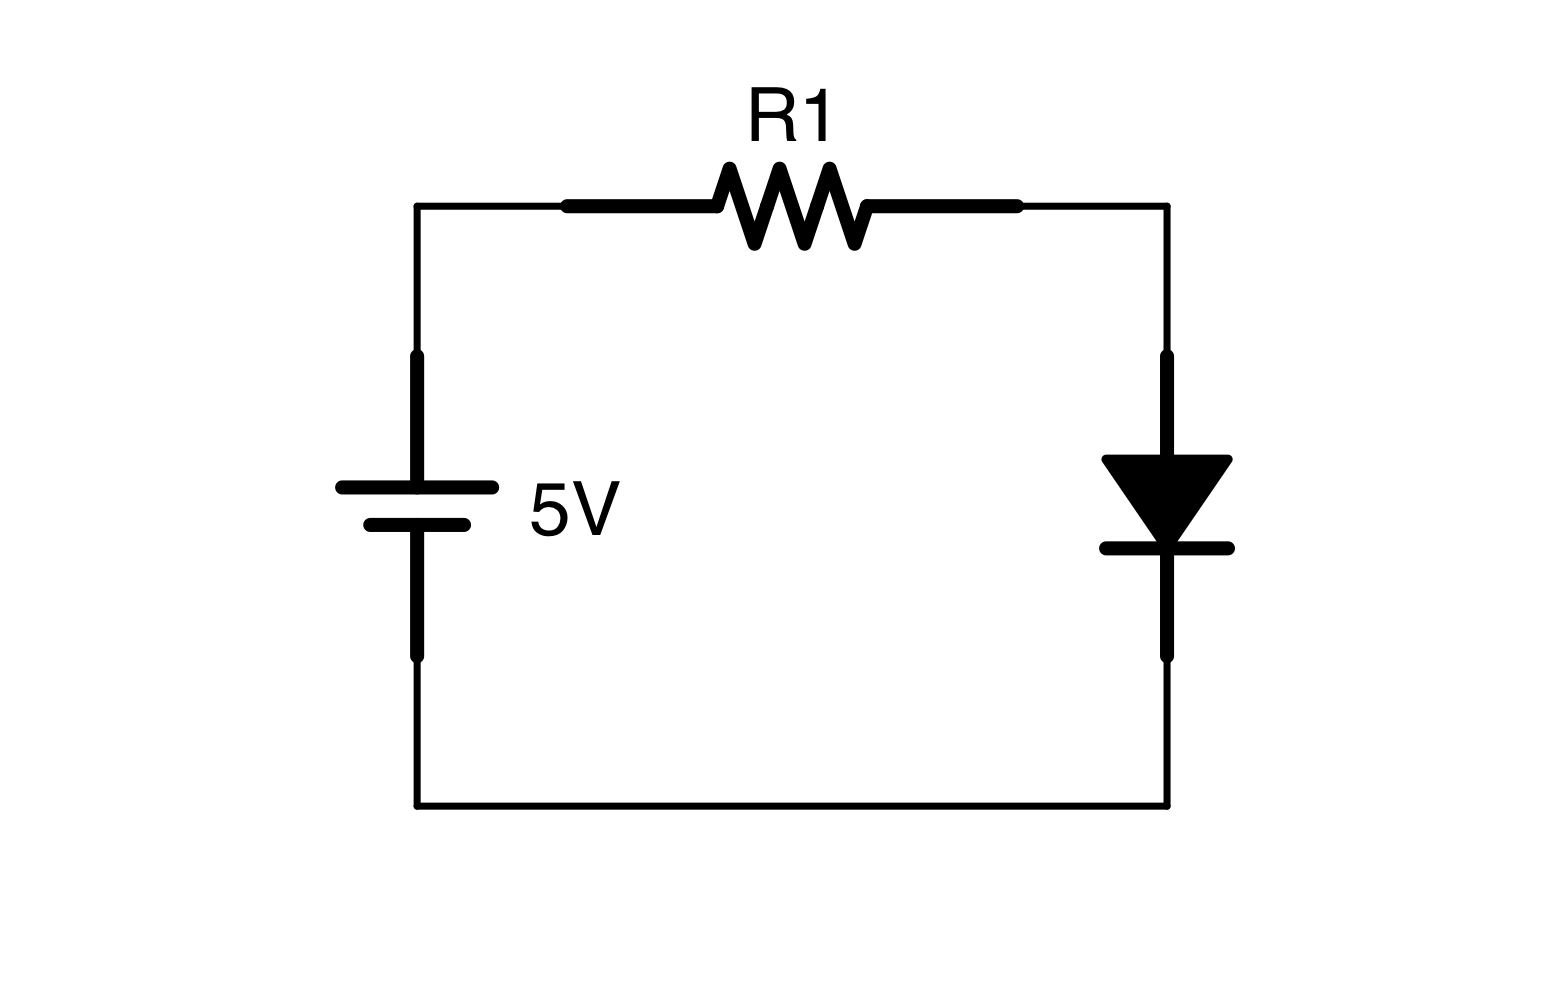
\includegraphics[scale=0.08]{DiodeApplyEx1.png}
\item Let's say instead of a standard diode, the diode is a blue LED.  Recalculate the current going through each component and the voltage drops for each component.
\item In the circuit below, calculate how much current is flowing through each component and each component's voltage drop if R1 is $300\myohm$, R2 is $400\myohm$, and R3 is $500\myohm$.  \\ 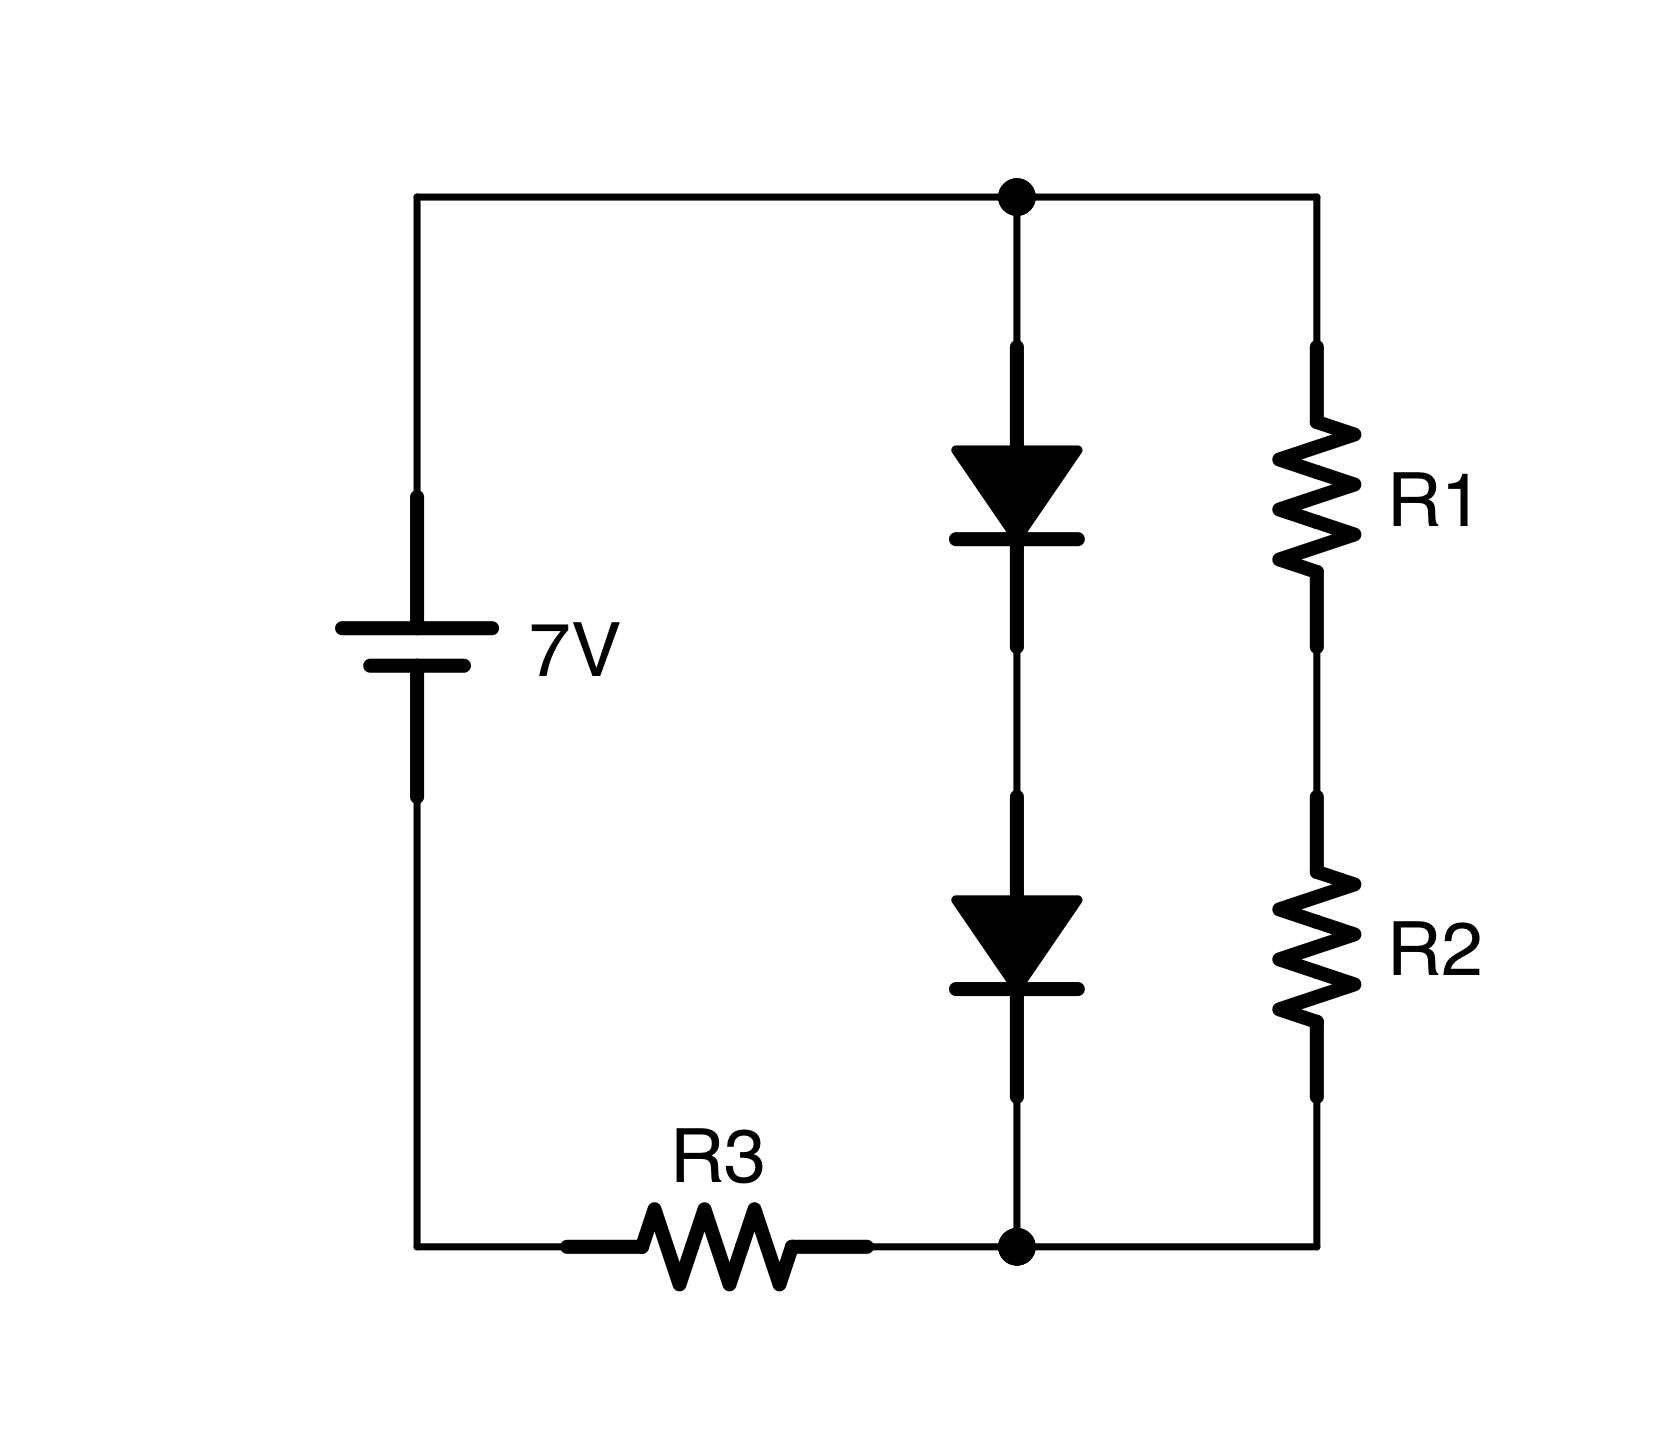
\includegraphics[scale=0.08]{DiodeApplyEx2.png}
\item Draw a circuit that provides a 6-volt regulated power supply to circuit load from a 9-volt battery using regular diodes.  Choose a resistor that works efficiently for a circuit load of $500\myohm$ and operates with a battery voltage from $7\myvolt$ to $9.6\myvolt$.  What is the current at the lowest and highest ranges of the battery?  How much is used by the circuit load and how much is wasted through the diodes in each configuration?
\item Draw an equivalent circuit to the previous question using a Zener diode instead of normal diodes.
\end{enumerate}

\chapter{Basic Resistor Circuit Patterns}
\label{chapBasicResistorCircuits}

When most people look at a schematic drawing, all they see is a sea of interconnected components with no rhyme or reason combining them.
However, most circuits are actually a collection of \glossterm{circuit patterns}.
A circuit pattern is a common way of arranging components to accomplish an electronic task.
Experienced circuit designers can look at a circuit and see the patterns that are being used.
Instead of a mass of unrelated components, a circuit designer will look at a schematic and perceive a few basic patterns being implemented in a coherent way.

In this chapter, we are going to learn three basic resistor patterns, and learn to work with switches as well.

\section{Switches and Buttons}
% FIXME - should I move this to another chapter that needs content?

Switches and buttons are very simple devices, but nonetheless we probably need to take a moment to explain them.
A switch works by connecting or disconnecting a circuit.
A switch in the ``off'' position basically disconnects the wires so that the circuit can't complete.
A switch in the ``on'' position connects the wires.

There are different types of switches depending on their operation.
The ones we are concerned with are called ``single pole single throw'' (SPST) switches, which means that they control only one circuit (single pole), and the only thing they do is turn it on or off (single throw).

\simplegraphicsfigure{Schematic Symbols for an SPST Switch (left) and an APST button (right)}{SwitchSchematicSymbols}{0.08}

Figure~\ref{figSwitchSchematicSymbols} show what the schematic symbols for an SPST switch and an SPST momentary switch (i.e., a button) look like.
As the drawing indicates, when the switch is open, the circuit disconnects.
When the switch closes, it connects the circuit.
While the switch holds its position stable (someone has to manually switch it back and forth), the button only connects the circuit \emph{while it is being pushed}.  
While the button is being pushed, the circuit is connect, but as soon as someone stops pushing the button, the circuit opens back up.

\simplegraphicsfigure{A Simple Switch Circuit}{SimpleSwitchCircuit}{0.08}

Figure~\ref{figSimpleSwitchCircuit} shows what a simple circuit with a switch looks like.
It is just like a normal LED circuit, but with a switch controlling whether or not electricity can flow.
Note that the switch is just as effective on the other side of the circuit.
If the switch was the last part of the circuit, it would be equally as effective.  
Remember, in order for current to flow, there must be a full circuit from positive back to negative.

\section{Current-Limiting Resistor Pattern}

The first resistor pattern we are going to learn is one that we already know---the current-limiting resistor pattern.
The idea behind this pattern is that a resistor is added to limit the amount of current that can flow through a device.
The size of the resistor needed depends on the size of the voltage source, the action of the device itself, and the maximum amount of current to allow.
Then, the resistor size needed can be calculated using Ohm's Law.

Many resistors are added to circuits to limit current flow.
At the beginning, we used resistors to make sure we didn't destroy our LEDs.
In Chapter~\ref{chapDiodes}, we used a resistor to limit the amount of current flowing through our voltage regulation circuit.

In many different circuits, we will need resistors to limit current for two different reasons---to avoid breaking equipment and to save battery life.
Oftentimes, we are actually choosing resistor values to accomplish both of these tasks.

If an LED breaks with $20\mymamp$, then we need a resistor big enough to keep the current that low.
However, if the LED light is sufficiently visible with $1\mymamp$, then, to save battery life, we might want a bigger resistor.
Battery capacity is often measured in milliamp-hours (mAh), with a typical $9\myvolt$ battery holding 400mAh.  
So, with such a battery, an LED circuit at $10\mymamp$ will drain the battery in 40 hours ($400\textrm{mAh} / 10\mymamp = 40\textrm{h}$), but the same LED circuit with a bigger resistor, limiting the current to $1\mymamp$ will take a full 400 hours ($400\textrm{mAh} / 1\mymamp = 400\textrm{h}$) to drain the same battery!
That will save you a lot of money in the long run.

\section{Voltage Divider Pattern}

\simplegraphicsfigure{A Simple Voltage Divider Circuit}{SimpleVoltageDivider}{0.08}

A \glossterm{voltage divider} occurs anytime there are two resistors together with a subcircuit coming out from in-between them.
They usually are connected to a fixed positive voltage on one side of the first resistor, and the ground on the other side of the second resistor, but this isn't strictly necessary.
A simple schematic of a voltage divider is shown in Figure~\ref{figSimpleVoltageDivider}.
Notice that there are two resistors between the voltage source and the ground (a 1k on top and a 2k on bottom) and a subcircuit (indicated by the load resistance) branching off from between them.
Under certain circumstances (which will be covered in a moment), we can basically ignore the parallel resistance of the subcircuit, and just look at the voltages at each point in the main voltage divider circuit.

We can see that the voltage at the top of the voltage divider is $9\myvolt$ (because it connects to the positive terminal) and at the bottom of the voltage divider it is $0\myvolt$ (because it connects to the negative terminal).  
Therefore, the total voltage drop across both resistors must be $9\myvolt$.
Since the resistors are in series (remember, we are ignoring the load for now), we can find the total resistance in the circuit by just adding their resistances.
So, $1,000\myohm + 2,000\myohm = 3,000\myohm$.
Since the current in a series is the same for the whole series, we can now use Ohm's Law to calculate the current flow:

$$ I = V / R = \frac{9\myvolt}{3,000\myohm} = 0.003\myamp = 3\mymamp $$

So, there is $0.003\myamp$ ($3\mymamp$) in this circuit.
That means that \emph{each} resistor in the series will have this amount of current flowing through them.
Therefore, we can calculate the voltage drop across each resistor.
Let's look at the 1k resistor:

$$ V = I * R = 0.003\myamp * 1,000\myohm = 3\myvolt $$

So, the voltage drop across the first resistor is $3\myvolt$.
That means that, since the battery started at $9\myvolt$, at the end of the resistor the voltage compared to ground is $6\myvolt$.
We can calculate the voltage drop across the second resistor either by Ohm's Law again or just by noting the fact that since the other end of the resistor is connected to ground, the voltage \emph{must} go from $6\myvolt$ to $0\myvolt$.

\simplegraphicsfigure{Voltage Divider with Voltages Labelled}{SimpleVoltageDividerLabelled}{0.08}

Figure~\ref{figSimpleVoltageDividerLabelled} shows the voltages at each point.
As you can see, the wire from the middle of the voltage divider has a new voltage that can be used by the load.
This is what voltage dividers are normally for---they provide a simple way of providing a scaled-down voltage to a different part of the circuit.

But how do we choose the values of the resistors?

One thing to note is that the second resistor consumed exactly twice as much voltage as the first resistor.
Additionally, the second resistor was exactly twice as large as the first resistor.
Thus, as a general principle, the relative sizes of the resistors will determine the relative amounts of voltage they eat up.
So, if we needed a $4.5\myvolt$ output, that is half of our input voltage.
Therefore, we would need both resistors to be the same.

A more explicit way of stating this is with an equation.
Given a starting voltage $V_{IN}$ connected to the first resistor, $R_1$, and the second resistor ($R_2$) connected to ground, the output voltage ($V_{OUT}$) coming out between the resistors will be given by the equation:

\begin{equation}
V_{OUT} = V_{IN} * \frac{R_2}{R_1 + R_2}
\end{equation}

Note that the specific values don't matter yet---it is the \emph{ratio} we are concerned about so far.
To get $4.5\myvolt$, we can use two $1\mykohm$ resistors, two $200\myohm$ resistors, or two $100\mykohm$ resistors.
As long as the values are the same, we will divide the voltage in half.

If we wanted an $8\myvolt$ output, we would do a similar calculation.  
Since we start at $9\myvolt$, we need to use up $\frac{1}{9}$ of the voltage in the first resistor, and $\frac{8}{9}$ of the voltage in the second resistor.
Therefore, our resistors need to be in similar ratio.
We could use an $100\myohm$ resistor for the first resistor, and a $200\myohm$ resistor for the second resistor.

So how do you determine exactly what value to use?
Here is where we start thinking about the load again.
While we have been treating the voltage divider as a series circuit, in truth we have one resistor in series, and then a parallel circuit with the other voltage divider resistor in parallel with the load.
Our simplified model (where we ignore the parallel resistance) will work, \emph{as long as the load resistance does not impact the total parallel resistance by a significant amount}.
Therefore, let's look at how the load resistance affects the parallel resistance.

So, using Equation~\ref{eqparallelresistancen} we can write a formula for the total resistance of these two, with $R_2$ being our second voltage divider resistor and $R_L$ being our load resistance:

$$ R_T = \frac{1}{\frac{1}{R_2} + \frac{1}{R_L}} $$

Now, let's look back at the circuit in Figure~\ref{figSimpleVoltageDividerLabelled}.
Let's say that the resistance of the load ($R_L$) is $400\myohm$, which is much less than the resistance of the voltage divider resistor ($R_2$).
So what is the total resistance?

$$ R_T = \frac{1}{\frac{1}{R_2} + \frac{1}{R_L}} = \frac{1}{\frac{1}{2,000} + \frac{1}{400}} = \frac{1}{0.0005 + 0.0025} = \frac{1}{0.003} \approx 333\myohm $$

This is way off of our simplified model which ignored the load resistance, which gave $2,000\myohm$.
Now, let's increase the load resistance so that it is equal to the load resistance ($2,000\myohm$) and recalculate:

$$ R_T = \frac{1}{\frac{1}{R_2} + \frac{1}{R_L}} = \frac{1}{\frac{1}{2,000} + \frac{1}{2,000}} = \frac{1}{0.0005 + 0.0005} = \frac{1}{0.001} \approx 1,000\myohm $$

This is still significantly off, but it is much closer.
So, now, let's look at what happens if the load resistance is double of $R_2$, or $4,000\myohm$:

$$ R_T = \frac{1}{\frac{1}{R_2} + \frac{1}{R_L}} = \frac{1}{\frac{1}{2,000} + \frac{1}{4,000}} = \frac{1}{0.0005 + 0.00025} = \frac{1}{0.00075} \approx 1,333\myohm $$

Here, we are getting much closer to our original value.  Now, let's say that the load is ten times the resistance of our $R_2$ resistor, or $20,000\myohm$.  That give us this:

$$ R_T = \frac{1}{\frac{1}{R_2} + \frac{1}{R_L}} = \frac{1}{\frac{1}{2,000} + \frac{1}{20,000}} = \frac{1}{0.0005 + 0.00005} = \frac{1}{0.00055} \approx 1,818\myohm $$

This is very close to the resistance of $R_2$ by itself.
So, what we can say is that our voltage divider circuit can ignore the resistance of the load \emph{if the resistance of the load is significantly more than the resistance of the voltage divider resistor}.
A way of writing this down is that $R_L >> R_2$.
What ``significantly'' means depends on how sensitive your circuit it to voltage changes, but, generally, I would say that $R_L$ should be at least ten times $R_2$.

So, for low-resistance loads, a voltage divider does not work well, because it puts too little resistance between the voltage source and ground.
However, in Chapter~\ref{chapIC} we will see that many circuit have loads of approximately infinite resistance, so voltage dividers work well.

In general terms, a voltage divider with smaller resistors is ``stiffer'' because it varies less in response to variations in a load, but it also eats up more current.
A voltage divider with larger resistors doesn't work with low-resistance loads, but it also uses up much less current.

\section{The Pull-Up Resistor}
\label{secPullUpResistor}

The pull-up resistor is a strange circuit, but we will find very good applications for it once we start dealing with ICs in Chapter~\ref{chapIC}.
It is probably easiest to describe by simply showing you a circuit and then describing how it works.

\simplegraphicsfigure{Basic Pull-Up Resistor}{PullUpResistorBasic}{0.08}

Figure~\ref{figPullUpResistorBasic} shows the circuit diagram for a basic pull-up resistor circuit.
Normally, we think of lighting up an LED by pushing the button.
However, in this case, pushing the button causes the current to bypass the LED.

If you look at the path from where the circuit branches, when the button is not pressed, the current can only go one way---through the LED.
However, when the button is pressed, the electricity has two options---either through the LED or directly to ground through the button.
The electricity would always rather go directly to ground rather than through an intermediary, so \emph{all} of the current goes through the closed button, and none of it goes through the LED.

Since the branch point is directly connected to ground when the button is pushed, that means that the voltage \emph{at the branch point} is also zero.
Kirchoff's Voltage Law says that no matter what path is taken, the voltage drop will always be the same.
However, an LED induces a voltage drop, but the voltages on both sides of the LED are zero.
Therefore, electricity cannot flow through the LED.

So what is the function of the resistor?
The resistor connects the switch and the LED to the positive voltage source, and provides a limitation on the current that runs through it.
The resistor must be \emph{before} the branch point for it to work.

Think about what happens without the resistor, or if the resistor is after the branch point.
The electricity will have a path directly from the positive voltage source to ground with no resistance---in other words, a short circuit.
This will draw an enormous amount of electricity.
Figure~\ref{figPullUpResistorBad} shows what this would look like.
Notice that when the button is pushed, you can trace a path from the positive voltage source to ground with no intervening resistance.

\simplegraphicsfigure{Incorrect Way to Wire the Circuit}{PullUpResistorBad}{0.08}

The resistor is called a pull-up resistor because it is connected to the positive voltage source, and is used to ``pull up'' the voltage on the circuit to a positive value when the switch is open.
In Chapter~FIXME we will look at resistors that are connected to ground, called pull-down resistors.

In short, a pull-up resistor is usually used to supply positive voltage to a circuit which might be turned off by redirecting the voltage to ground.
The resistor provides both the electrical connection to the positive source and a limit to the amount of current that will flow if the wire is then routed to ground (usually through some kind of switching mechanism).

\reviewsection

In this chapter, we learned:

\begin{enumerate}
\item Most circuits are a combination of common, well-understood circuit patterns.
\item The more experienced you are with circuits, the easier it is to see these circuit patterns when you look at a schematic drawing.
\item A current-limiting resistor is a resistor that is used to limit the maximum current flow within a circuit, either to protect other components or to limit overall electricity usage.
\item A voltage divider is a pair of two resistors connected in series with one another (usually connected to a positive voltage on one side and the ground on the other), but with another wire coming out in-between them to provide voltage to another circuit (called the \emph{load}).
\item In a voltage divider, it is assumed that the resistance of the load is significantly more than the resistance of the second half of the voltage divider because then the load can be basically ignored for calculating voltage drops.
\item For a voltage divider, the ratio of the voltages consumed by each resistor is the same as the ratio of their resistances.  The output voltage coming out between them is the same as the voltage used by the second resistor.
\item Another way of stating the output voltage is $V_{OUT} = V_{IN} * \frac{R_2}{R_1 + R_2}$, where $R_1$ is the resistor connected to the positive voltage and $R_2$ is the resistor connected to ground.
\item Voltage dividers with smaller resistances are ``stiffer''---they are impacted less by the resistance of the load.  Voltage dividers with larger resistances waste much less current.
\item A pull-up resistor circuit is a circuit in which a positive voltage which may be switched to ground at some point is provided through a resistor.
\item The pull-up resistor both (a) connects the circuit to the positive voltage to supply a positive current when the circuit is not switched to ground and (b) limits the current going to ground (i.e., prevents a short circuit) when the load is switched to ground.
\item It is called a pull-up resistor because it pulls the voltage up when the circuit is not switched to ground.
\end{enumerate}

\applysection

\begin{enumerate}
\item Given a $15\myvol$ voltage supply, what size of a resistor would be needed to make sure that a circuit never went over $18\mymamp$.
\item Given a $9\myvolt$ battery source, design a voltage divider that will output $7\myvolt$ to a load that has a resistance of $10\mykohm$.
\item Given a $3\myvolt$ battery source, design a voltage divider that will output $1.5\myvolt$ to a load that has a resistnace of $1\mykohm$.
\item In Figure~\ref{figPullUpResistorBasic}, how much current is going through the circuit when the switch is open?  How much when it is closed?
\item How would you modify the circuit in Figure~\ref{figPullUpResistorBasic} to keep the maximum current in the circuit under $2\mymamp$?
\end{enumerate}

\chapter{Integrated Circuits and Resistive Sensors}
\label{chapIC}

So far, the components we have studied are simple, basic components---batteries, resistors, diodes, etc.
In this chapter, we are going to start to look at \glossterm{integrated circuits}, also called \glossterm{chips}, \glossterm{microchips}, or \glossterm{IC}s.
An IC is a miniaturized circuit placed on silicon.
It is a whole collection of parts geared around a specific function.
These functions may be small, such as comparing voltages or amplifying voltages, or they may be complex, such as processing video or even complete computers.
A single chip may hold just a few components, or it may hold billions.

Miniaturized circuits have several advantages---they are cheaper to produce in mass, they use less power, and they take up less space in your overall circuit---all because they have a reduced area and use fewer materials.
These miniaturized circuits are what allowed for the computer revolution over the last century.

\section{The Parts of an Integrated Circuit}

Integrated circuits, as we have noted, are basically miniaturized circuits placed on a siliconplate, called the die.
This die is where all of the action of the integrated circuit takes place.

The die is then placed into a \glossterm{package}, which then provides connection points for circuit designers to interface with the IC.
These connection points are often called \glossterm{pins} or \glossterm{pads}.
Each pin on an IC is numbered, starting with pin 1 (we will show you how to find pin 1 shortly).
Knowing which pin is which is important, because most of pins on a chip each have their own purposes, so if you attach a wire to the wrong pin your circuit won't work, or you will destroy the chip.
Most packages are marked with the chip's manufacturer and part number.

There are many different types of packaging available, but there are two general types that are often encountered:

\begin{description}
\item[Through-Hole] In this packaging type, the connection points are long pins which can be used on a breadboard.  This type of packaging is easiest for amateur usage.
\item[Surface Mount]  In this packaging type, the connection points are small pads which are meant to be soldered to a circuit board.  This packages are much smaller (and therefore less expensive), and can be more easily managed by automated systems.  These are also referred to as SMD (surface mount devices) or SMT (surface mount technology).
\end{description}

\simplegraphicsfigure{Comparison of the Same IC in SMD (left) and DIP (right) Packages}{DIPAndSMD}{0.125}

Since we are only using breadboards in this book and not doing any soldering, we will only concern ourselves with through-hole packaging.
However, through-hole packaging itself comes in a variety of styles.
The main one we will concern ourselves with is called a \glossterm{dual in-line package}, or \glossterm{DIP}.  

\simplegraphicsfigure{Pin 1 is Immediately Counterclockwise of the Notch}{FindPin1}{0.125}

An Integrated Circuit in a DIP package has two rows of pins coming out of the package.
Most chips mark either the top of the chip with a notch or indentation (where pin 1 is immediately counterclockwise of the notch), or mark pin 1 with an indentation, or both. 
See Figure~\ref{figFindPin1} to see how to use the notch to find pin 1.
The rest of the pins are numbered counterclockwise around the chip.

\simplegraphicsfigure{A DIP IC Inserted Into a Breadboard}{ChipInBreadboard}{0.125}

The beauty of a DIP packaged IC is that it fits perfectly onto most breadboards.
Figure~\ref{figChipInBreadboard} shows how you can place your IC across the breadboard's bridge and each pin on the chip will have its own terminal strip to connect to.

Be careful, though, when inserting ICs into breadboards.
The pins on an IC are often slightly wider than the breadboard.
If you just jam the IC into the breadboard, you will likely accidentally crush one or more of the pins that aren't exactly aligned on the hole.
Instead, compare the width of the pins to the width it has to fit in on your breadboard.
If it doesn't match up, \emph{very gently} bend the pins with your fingers or with pliers to get them to match up.

Usually, the ICs that I purchase are just a little wide, and I will squeeze the pins on each side slightly between my thumb and finger until they move close enough together.
However, you adjust the pins, make sure they line up before pushing them into their connection points on the breadboard.
Also, with larger ICs, you may need to adjust the IC back and forth as you gently insert it into place on the breadboard.

\section{The LM393 Voltage Comparator}

There are thousands and thousands of available chips which do a dizzying array of functions.
In this chapter, we are going to focus on a very simple chip---the LM393 Voltage Comparator.
This chip does one simple task.
The LM393 compares two input voltages, and then outputs either a high-voltage signal or a low-voltage signal depending on which input voltage is greater.
The LM393 is actually a \emph{dual} voltage comparator, which means that it will do two separate comparisons on the same chip.
Like most chips, the LM393 is an \emph{active} device, which means that it additionally requires a voltage source and a ground connection to provide power to the device.

\simplegraphicsfigure{The Pin Configuration of an LM393}{lm393Pinout}{0.25}

Figure~\ref{figlm393Pinout} shows the pin configuration (also called the \glossterm{pinout}) of the LM393.
The first thing to note on any pinout is where the voltage and ground connections are.
In this case, the voltage is marked as $V_{CC}$ and the ground is marked as $GND$.
Even though the LM393 has \emph{two} voltage comparators on the chip, they both share the power ($V_{CC}$) and ground ($GND$) pins.
The left side of the chip diagram shows the inputs and output for the first voltage comparator ($1IN+$, $1IN-$, and $1OUT$), and the inputs and output for the second voltage comparator is on the right ($2IN+$, $2IN-$, and $2OUT$).
In your projects, you can use whichever one is more convenient for you, or even both at the same time.

So, the \icode{1IN+} pin (pin 3) and the \icode{1IN-} pins are where the two voltages are being fed that are being compared by the first comparator.
The \icode{1OUT} is the pin which will contain the output.
If the voltage at \icode{1IN+} is less than the voltage on \icode{1IN-}, the output pin will be at a low (i.e., zero/ground) voltage.
If the voltage at \icode{1IN+} is greater than the voltage on \icode{1IN-}, the output pin \emph{will not conduct at all}, but this will be considered a ``high'' (positive-voltage) state.
This sounds counterintuitive, but, as we will see, this lets us set our own output voltage to whatever we want without causing too much complexity.
This configuration where high-voltage outputs don't conduct is called an \glossterm{open collector} configuration.
Don't worry if this is a little confusing, we will discuss it more in-depth later in the chapter.

\begin{sidebar}[Voltage Sources on Integrated Circuits]
Note that the voltage pins on integrated circuits can be marked in a number of different ways.
The positive voltage source is often labelled as $V_CC$, $V_DD$, or $V_+$.
The ground connect is often labelled as GND, $V_EE$, $V_SS$, or $V_-$.
There are additional ways that these are labelled as well.
Finding the positive and ground connections for an IC should always be the first thing you do with them.
\end{sidebar}

\section{The Importance and Problems of Datasheets}

Every IC (and, usually, any other part as well) has a datasheet supplied by the manufacturer which tells you important details about how you should use their chip in your circuit.
Reading datasheets is one of the worst parts of electronics, in my opinion. 
For me, datasheets rarely have the information I am actually looking for in a way that is easy to find.

In fact, most datasheets assume that you already know how to use the device, and the datasheets are just there to supply additional details about the limitations of the device.
For instance, looking through the LM393 datasheet from Texas Instruments, the actual operation of the device isn't even listed until page 11, and there it is buried within a sub-subsection, almost as a side-note.

These datasheets are written by people who have spent a lot of time being electrical engineers, and they are written for people who have spent a lot of time being electrical engineers, so when mere mortals read the datasheets, the important pieces are often shrouded in unintelligible gibberish.
For instance, the fact that the ``high'' output state of the device doesn't conduct isn't mentioned explicitly anywhere at all in the datasheet.  
Instead, it is implied by the configuration.

The reason for this is that the datasheets are usually read by professionals familiar with the type of device, and just need to know the electrical details so they don't accidentally bend the device beyond the breaking point.
Thus, the datasheets oftentimes spend more time just showing and describing the layout of the circuit on the chip and graphs of different chip properties, and then you are left to interpret what that means for your circuit.
For advanced circuit designers, this is great.
For students and hobbyists, however, this is oftentimes more frustrating than helpful.

However, datasheets do often provide a few basic details that are helpful to everyone.
They will often tell you:
\begin{itemize}
\item What each pin does
\item What the power requirements are
\item What the outer limits of the chip's operation are
\item An example circuit that you can build with the device
\end{itemize}

For all of these reasons, Appendix~\ref{appSimplifiedDatasheets} contains simplified datasheets for a number of common devices that are easier to read than the standard ones. 

For the LM393, the important points are:

\begin{enumerate}
\item The input voltage on $V_{CC}$ can be anywhere between $2\myvolt$ and $36\myvolt$.
\item When sensing voltage, the LM393 doesn't really draw any (or at least much) current, so there are no parallel resistances we need to worry about.
\item The output is high when \icode{IN+} is greater than \icode{IN-}, and low (i.e., ground) when \icode{IN+} is less than \icode{IN-}, with an error range of about 2 millivolts.
\item When the output is low, the output pin will conduct current into itself (since it is at ground, positive charge will naturally flow into it), but if sink more than $6\mymamp$ into it, you will destroy it.
\item When the output is high, the device will not conduct any current.
\end{enumerate}

That isn't to say that the datasheets aren't important, but for a beginner the datasheets usually aren't what you need to get started.

\section{A Simple Circuit with the LM393}

In this section, I am going to show a simple circuit using the LM393 chip.
In doing so, we are going to be using several of the resistor circuit patterns that we learned in Chapter~\ref{chapBasicResistorCircuits}.

\simplegraphicsfigure{A Simple Comparator Circuit}{SimpleComparatorCircuit}{0.08}

The circuit we are discussing is shown in Figure~\ref{figSimpleComparatorCircuit}.
Can you identify the resistor circuit patterns?  
Take a minute and see if you can find some.
Note that the wire coming out of \icode{1IN-} crosses two wires that it is \emph{not} joined with.

The first thing to notice is that we have \emph{two} voltage dividers.
The first voltage divider is between R1 and R2.
Since R1 and R2 are the same resistance and are connected to both $9\myvolt$ and $0\myvolt$, that means that they divide the voltage in half, giving a $4.5\myvolt$ output.
The second voltage divider is between R3 and R4.
Since R3 is half of the resistance of R4, that means that it only uses up half as much voltage as R4.  
Thus, since R3 eats up $3\myvolt$ and R4 eats up $6\myvolt$, the wire coming out from the middle is at $6\myvolt$.

Then, to the right of the circuit, you can see that we have a current-limiting resistor in front of the LED.
That is not its only function, though.
It also functions, as we will see shortly, as a pull-up resistor.

So what is the big triangle?
Comparators (and several other circuits commonly placed on ICs) are represented as triangles in the schematic (we could have also placed the chip itself there).
Each of the connections are labelled the same as they are labelled in the pinout diagram in Figure~\ref{figlm393Pinout} so they would be easy to locate.

The way that the circuit works is very simple.
The voltage coming in to \icode{1IN+} is $6\myvolt$ and the voltage coming in to \icode{1IN-} is $4.5\myvolt$.
Since \icode{1IN+} is greater than \icode{1IN-} then that will turn \icode{1OUT} to high (positive voltage).
However, remember that we said that \icode{1OUT} \emph{does not conduct} when it is high.
It acts like an open switch.
Therefore, R5 acts like a pull-up resistor and supplies the positive voltage for us to our LED to turn it on.

Now let's say that the input voltages were reversed.
What would happen?
If \icode{1IN-} is greater than \icode{1IN+}, then \icode{1OUT} will go low (zero volts) and also conduct.
It will act like a closed switch going to ground.

Therefore, current will go the easy route - it will go through \icode{1OUT} (directly to ground) instead of through the LED ($1.8\myvolt$ or more).
This works just like the switch in the circuit in Section~\ref{secPullUpResistor}.
When \icode{1OUT} is low, it acts like a closed switch to ground.
When \icode{1OUT} is high, it acts like an open switch (and is whatever positive voltage you supply yourself).

The resistor R5 does several jobs.
The first job is to act as a pull-up resistor. 
Remember that a pull-up resistor prevents the load to ground from going too high when the switch is closed.
Without the pull-up resistor, when the switch is closed (\icode{1OUT} goes low), we would have a short-circuit from the voltage source to ground.
This would not only waste a large amount of electricity, it would break the LM393, because it can only sink a maximum of $6\mymamp$ of current.
Having a $3\mykohm$ resistor, we limit the current for the closed switch to $I = V / R = 9 / 3,000 = 0.003A = 3\mymamp $.

When the switch is open, the current flows through the resistor to the LED, and then the resistor acts as a current-limiting resistor for the LED.
The amount of current to the LED will be calculated as $I = V / R = (9 - 1.8) / 3,000 = 7.2 / 3,000 = 0.0024\myamp = 2.4\mymamp$.

\section{Resistive Sensors and Voltages}

One of the more practical uses of the voltage comparator circuit is to measure the values of sensors which act as variable resistors.
Many different materials in the world act as resistors.
What's really interesting is that many of these materials \emph{change their resistance} depending on external factors.
Some of them change their resistance based on temperature, pressure, light, humidity, and any number of other environmental factors.

Now, changing resistance doesn't tell us much by itself.
If we put a resistor between a voltage source and ground, it will always eat up that voltage source.
However, if you use it in concert with a fixed resistor to make a voltage divider, you can then get the output voltage to vary based on the changes in resistance.

\simplegraphicsfigure{A Simple Resistor Sensor Circuit}{SimpleResistiveSensorCircuit}{0.08}

Figure~\ref{figSimpleResistiveSensorCircuit} illustrates this principle.
It is a simple voltage divider, where the top resistor is actually a photoresistor (a resistor that varies based on light) and the bottom resistor has a fixed resistance.
Thus, as the light varies, the top resistance will vary.
This will change the ratio between the top and bottom resistor, which will affect the output voltage.

To use this circuit, you will need to know the resistances of your photoresistor on the different conditions you are interested in.
I usually use the GL5528, which ranges from $10\mykohm$ in bright light to $1\myMohm$ in complete darkness.
However, depending on your specific photoresistor as well as the light conditions that you think of as ``light'' and ``dark,'' the resistance values that are relevant for light and dark will be different for you.
So, whatever photoresistor you use, it is worthwhile to measure the resistance using your multimeter in the different conditions you think of as light and dark.

\section{Sensing and Reacting to Darkness}

So far in the book, we have focused entirely on example circuits that didn't really do anything.
They lit up, they had voltage and current, but there wasn't much interesting that they were doing.
However, now, we finally have enough knowledge to start building circuits that \emph{do} something.

We have:
\begin{enumerate}
\item A way to generate a fixed voltage (using a voltage divider)
\item A way to generate resistances from real-world events (photoresistors and other resistance sensors)
\item A way to convert changes in resistances to changes in voltage (using a voltage divider with one fixed resistor)
\item A way to compare our varying voltage to our fixed voltage (using the LM393 comparator)
\item A way to utilize the output signal from the LM393 to do work (using the pull-up resistor and the LED)
\end{enumerate}

There are a lot of pieces to put together this simple circuit, which is why it has taken so long to do anything worthwhile. 
However, if you have followed along carefully, now that you are here you should be able to see how all of this fits together.

What we will do is to take the circuit given in Figure~\ref{figSimpleComparatorCircuit} and modify R4 to be our photoresistor and R3 to be a fixed resistor.
In my own testing, I discovered that the light/dark switchover point for my photoresistor was about $15\mykohm$.
Therefore, I am going to use a $15\mykohm$ resistor as the fixed resistor for R3.
Yours may need to vary based on your experimentation with your photoresistor.

When the light is on, my photoresistor will have a lower resistance than $15\mykohm$, which will make the fixed resistor R3 use up more of the voltage.  
Thus, the voltage at the divider will be less than $4.5\myvolt$, which will turn \icode{1OUT} to low (which closes the switch and makes a path to ground on the output before it gets to the LED, which turns the LED off).

In low-light conditions, the resistance will jump way up above the resistance of the fixed resistor.
If the upper, fixed resistor has less resistance than the bottom resistor, then the voltage at the divider will be larger than $4.5\myvolt$, activating the comparator and turning \icode{1OUT} to high (i.e., opening the switch and allowing power to flow through the LED).

The final circuit is given in Figure~\ref{figDarknessSensorCircuit}.
You can see a way to lay it out on the breadboard in Figure~\ref{figDarknessSensorBreadboard}.

\simplegraphicsfigure{Darkness Sensor Schematic}{DarknessSensorCircuit}{0.08}

\simplegraphicsfigure{Darkness Sensor Breadboard Layout}{DarknessSensorBreadboard}{1}

\section{Sources and Sinks}

Two terms that often come up when dealing with circuits are the concepts of a current \glossterm{source} and a current \glossterm{sink}.
A source is a component whose pins might provide current to other parts of the circuit.
A sink is a component whose pins might pull current from other parts of the circuit.

For the LM393, its input pins neither source nor sink current (at least not any significant amount).
The input pins more-or-less just sense the voltage without pulling any measurable current.
Therefore, they are neither sources nor sinks of current.
Technically, they probably sink a few nanoamps (billionths of an amp), but not nearly enough to affect our circuit analysis.

The output pin, even though it is called an \emph{output}, doesn't source any current.  
Instead, it acts either as a sink (when low) or as a disconnected circuit (when high).
This is known as an \glossterm{open collector} output.

Anytime an IC sources or sinks current, be sure to read the datasheets on the maximum amount of current it can source or sink.
These are usually quantities that \emph{you} have to limit---they are merely telling you at what point their circuit will physically break.
Therefore, you must use resistors to limit the currents to make sure that they are within limits.

However, be aware that many (but certainly not all) ICs do not source current, using open collectors for their output operations.
This has the disadvantage that you have to supply your own voltage and pull-up resistor to the output pin, but it also has the advantage that the output is set to \emph{whatever voltage level you choose}.
In other words, you don't need to pick a new comparator IC to get a different output voltage.

\reviewsection

In this chapter, we learned:

\begin{enumerate}
\item Integrated Circuits (called ICs or chips) are miniaturized circuits packaged up into an a single chip that can be added to other circuits.
\item ICs can have a few or several billion components on them, depending on the function.
\item ICs have different types of packages, including through-hole (optimized for breadboards) and surface mount (optimized for soldering and machine placement).
\item Dual In-line Packages (DIP) are the most common through-hole packaging type used for students, hobbyists, and prototype-builders.
\item DIP chips should be placed in the breadboard saddling the bridge, so that each IC pin is attached to its own terminal strip.
\item On most chips, pin 1 is located immediately counterclockwise of the notch in the chip, and remaining pins are numbered counterclockwise.
\item Most ICs are active devices, meaning that they have a direct connection to a power supply in addition to their input and output pins.a
\item An ICs Datasheet is a document that tells about the electrical characteristics of an IC.  However, most of them are difficult to read and assume you are already familiar with the part.  However, they are very useful for getting a pinout for the chip as well as telling the maximum ratings for voltages and currents.
\item The LM393 is a dual voltage comparator IC---it compares two voltages and alters its output based on which is larger.
\item The LM393's inputs do not consume any significant current on them when sensing the input voltages.
\item The LM393's outputs are open collectors---which means that they act as a switch to ground.  When the output is ``low'' the pin acts as a closed switch to ground.  When the output is ``high'' the pin acts as a disconnected circuit.
\item Because the LM393 acts as a disconnected circuit when high, a pull-up resistor circuit is required to get an output voltage.
\item Many sensors are based on the fact that the resistance of many materials will change with environmental factors.  Therefore, the sensor acts as a variable resistor, with the resistance telling you about the environment.
\item A resistive sensor can be used with a fixed resistor to make a variable voltage divider, essentially converting the resistance to a voltage.
\item By putting the resistive voltage divider in comparison with a fixed reference, we can use the LM393 comparator to trigger an output when the sensor crosses some threshold of resistance.
\end{enumerate}

\applysection


\begin{enumerate}
\item  Calculate the amount of current flowing through each element of the circuit in Figure~\ref{figSimpleComparatorCircuit}.  You can presume that the LM393 uses about $1\mymamp$ for its own operation, and that the LED is a red, $1.8\myvolt$ LED.  What is the total amount of current used by the circuit?
\item Take the circuit in Figure~\ref{figSimpleComparatorCircuit} and swap which voltage divider is attached to \icode{1IN+} and \icode{1IN-}.  Now calculate the total amount of current used by this circuit.
\item The Spectra Flex Sensor is a resistive sensor that changes its resistance when bent.  When it is straight, it has a resistance of $10\mykohm$.  When it is bent, it has resistances of $60\mykohm$ and above.  Draw a circuit that turns on an LED when the resistor is bent.  You may invent your own symbol for the flex sensor.
\item Build the circuit in Figures~\ref{figDarknessSensorCircuit} and~\ref{figDarknessSensorBreadboard}. 
\item If you wanted to wait until the room was even darker before the LED went on, how would you change the circuit?
\end{enumerate}



\appendix

\chapter{Glossary}
\label{chapGlossary}

\begin{description}
\item[AC current] See \emph{alternating current}.
\item[AC mains current] This is the type of current that is supplied to your house by the public utility companies.  This is usually 120 volts AC and cycles back and forth 50--60 times per second.
\item[AC signal current] This is the type of current usually picked up by a microphone or antenna.  It has very low current and usually must be amplified before processing.
\item[alternating current]
\item[amp] A shorthand way of saying ampere.  See \emph{ampere}.
\item[ampere] An ampere is a measurement of the movement of charge.  It is equivalent to one coulomb of charge per second moving past a given point in a circuit.
\item[charge] Charge is a fundamental quantity in physics.  A particle can be positively charged (like a proton), negatively charged (like an electron), or neutrally charged (like a neutron).  Charge is measured in coulombs.
\item[conventional current flow]
\item[coulomb] A coulomb is a quantity of electric charge.  One coulomb is roughly equivalent to the charge of $6.242×10^18$ protons.  The same number of electrons produces a charge of $-1$ coulomb.  Coulombs are represented by the symbol C.
\item[DC current] See \emph{direct current}.
\item[direct current]
\item[electron current flow]
\item[electron] A negatively-charged particle that is usually on the outside of an atom.
\item[milliamp] A short way of saying milliampere.  See \emph{milliampere}.
\item[milliampere] One thousandth of an ampere.  See \emph{ampere}.
\item[neutron] An uncharged particle in the nucleus of an atom.
\item[nucleus] The nucleus is the part of the atom where protons and neutrons reside. 
\item[proton] A positively-charged particle in the nucleus of an atom.

\end{description}

\chapter{Finding Component Values}

Since electronic components are so small and oddly-shaped, manufacturers have had to come up with some strange systems to let you know what values your components hold.
This appendix will tell you how, in most cases, to tell the values of different components.

\section{Resistors}
\label{appendixResistorValues}

\chapter{Electronics Symbols}
\label{appendixSymbols}

\begin{center}
\begin{tabular}{M{0.1\linewidth} | M{0.12\linewidth} | m{0.6\linewidth}}
\textbf{Symbol} & \textbf{Component} & \textbf{Description} \\

\includegraphics[scale=0.125]{BatterySymbol.png} & Battery & A battery is represented by a long line and a short line stacked on top of each other.  Sometimes, there are two sets of long and short lines.  The long line is the positive terminal and the short line is the negative terminal (which is usually used as the ground). \\ \hline
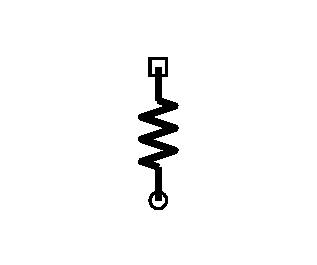
\includegraphics[scale=0.25]{ResistorSymbol.pdf} & Resistor & A resistor is represented by a sharp, wavy line with wires coming out of each side. \\ \hline
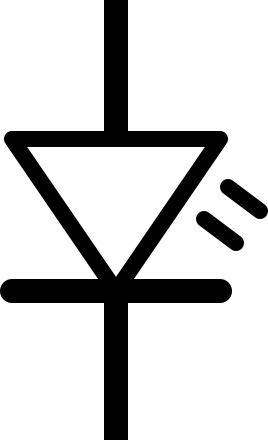
\includegraphics[scale=0.125]{LEDSymbol.png} & LED & An LED is represented by an arrow with a line across it, indicating that current can flow from positive to negative in the direction of the arrow, but it is blocked going the other way.  The LED symbol also has two short lines coming out of it, representing the fact that it emits light. \\
\end{tabular}
\end{center}


\chapter{Electronics Equations and Where They Come From}
\label{appendixElectronicsEquations}

% Thevenin Equivalent Equation
% Gain resistor equation

This appendix is a catalog of equations in electronics and where they came from for those who are curious.
This book is meant more for an introductory approach, but nonetheless many people are curious.
This chapter isn't for the faint of heart, and it may involve lots of math you haven't taken.
That's why it is stuck in an appendix.

However, if you are curious, these are the mathematical answers to your questions.

\section{Basic Formulas}

\subsection{Charge and Current Quantities}

\begin{itemize}
\item $1\textrm{ coulomb}  = 6.241509×10^18\textrm{ electrons}$ (how many electrons in a coulomb)
\item $I = \frac{dC}{dt}$ (current is the derivative of charge with respect to time)
\item $1A = 1\frac{C}{s}$ ($A$ = ampere; $C$ = coulomb; $s$ = second)
\item $3.6C = 1 mAh$ ($C$ = coulomb; $mAh$ is milliamp-hour,  a common unit for batteries)
\end{itemize}

\subsection{Volt Quantities}

Volts are basically measures of energy per unit of charge. Volts are also known as electromotive force (EMF), or $\epsilon$.  Volts can be expressed in a number of ways:

\begin{itemize}
\item $V = \frac{J}{C}$ ($J$ = joules; $C$ = coulombs)
\item $V = \frac{\textrm{potential energy}}{\textrm{charge}}$
\item $V = \frac{N\cdot m}{C}$ ($N$ = newtons; $m$ = meters; $C$ = coulombs)
\item $V = \frac{kg\cdot m^2}{A\cdot s^3}$ ($kg$ = kilograms; $m$ = meters; $A$ = amperes; $s$ = seconds)
\item $V = \frac{d\phi}{dt}$ (Faraday's law of induction---voltage is the derivative of the flux of the magnetic field with respect to time)
\end{itemize}

\subsection{Resistance and Conductance Quantities}

Resistance is in ohm's.  The inverse of resistance is conductance (the ability of current to flow through a wire) and is measured in Siemens (S).  The Seimens unit is also called a mho (ohm spelled backwards), and is sometimes marked by an upside down omega (℧).

\begin{itemize}
\item $G = \frac{1}{R}$ ($G$ = conductance in siemens, $R$ = resistance)
\item $G = \frac{I}{V}$ ($G$ = conductance; $I$ is current; $V$ is voltage)
\item $R = \frac{V}{I}$ (Ohm's law)
\end{itemize}

Individual materials have a resistivity ($\rho$).

\begin{equation}
R = \rho \cdot \frac{\textrm{length}}{\textrm{cross-sectional area}}
\end{equation}

In other words, from beginning to end, resistance decreases with cross-sectional area, and increases with length.

\subsection{Ohm's Law}

$V$ is voltage (in volts), $I$ is current (in amperes), and $R$ is resistance (in ohms).

\begin{equation}
V = I\cdot R
\end{equation}

\subsection{Power}

$P$ is in Watts.  The following hold true for DC circuits.  For AC circuits, they hold true if the resistance is actually an impedance.

\begin{itemize}
\item $P = V\cdot A$
\item $P = I^2R$
\item $P = \frac{V^2}{R}$
\end{itemize}

\subsection{Capacitance}

Capacitance is the ability to store charge.

The fundamental equation for a capacitor:

\begin{equation}
Q = V\cdot C
\end{equation}

$Q$ is the amount of charge stored, $V$ is the voltage across the terminals, and $C$ is the capacitance in farads.

The derivative of this equation with respect to time is:

\begin{equation}
\frac{dQ}{dt} = \frac{dV}{dt}\cdot C
\end{equation}

Because current is the derivative of charge, we can then say:

\begin{equation}
I = C\frac{dV}{dT}
\end{equation}

The capacitance of capacitors is given by the equation:

\begin{equation}
C = \epsilon_r\epsilon_0\frac{A}{d}
\end{equation}

Here $C$ is capacitance, $\epsilon_r$ is the dielectric constant of whatever separates the capacitor's plates, $\epsilon_0$ is the dielectric constant of free space, $A$ is the area of the plates in square meters, and $d$ is the distance between the plates in meters.

\subsection{Inductance}

The fundamental equation for an inductor is:

\begin{equation}
\phi = L\cdot I
\end{equation}

Here, $\phi$ is the flux of the magnetic field in Webers, $L$ is inductance in henries, and $I$ is current in amperes.
The derivative gives you voltage:

\begin{align}
\frac{d\phi}{dt} = L\frac{dI}{dt} \\
V = L\frac{dI}{dt}
\end{align}

In other words, the voltage produced is proportional to the change in current.

The inductance of a coil of wire can be calculated by:

\begin{equation}
L = \frac{\mu \cdot N^2 \cdot A}{l}
\end{equation}

Where $N$ is the number of turns of wire, $A$ is the area of the coil, $l$ is the length of the coil, and $\mu$ depends on the core being used.

\section{Semiconductors}

Components made from silicon are known as semiconductors, and have very useful non-linear properties.

\subsection{Diodes}

Diodes do not have a fixed voltage drop like we assume in this book.  
It is an exponential function, but is steep enough to act like a fixed $0.6\myvolt$ voltage drop for most purposes.
The actual equation is:

\begin{equation}
I = I_S (e^{\frac{V}{\eta V_T}} - 1)
\end{equation}

$I_S$ is the saturation current (depends on the construction of the diode), $V$ is the voltage, $\eta$ is either 1 for germanium or 2 for silicon, and $V_T$ is known as the thermal voltage (the amount of voltage created just by particles moving around at a given temperature, usually about $0.026\myvolt$ at room temperature).

\subsection{NPN BJT Transistors}

While we discussed general rules about BJT transistors, the technical model used to model them is known as the Ebers-Moll model.
This model is much more complex to use, which is why we don't discuss it much in the chapter.

There are also several different Ebers-Moll models, depending on the level of detail required.
The basic Ebers-Moll model for a conducting but unsaturated transistor is as follows:

\begin{equation}
I_E = I_S(e^{\frac{V_BE}{V_T}} - 1)
\end{equation}

In this $I_E$ is the emitter current (you can also use it for the collector current, since they are approximately equal).
$I_S$ is the saturation current of the base-emitter diode, and $V_T$ is the thermal voltage, just like for diodes.

% http://people.seas.harvard.edu/~jones/es154/lectures/lecture_3/bjt_models/ebers_moll/ebers_moll.html
% http://inderjitsingh87.weebly.com/uploads/2/1/1/4/21144104/the__ebers-moll_bjt_model.pdf
% http://ecetutorials.com/analog-electronics/ebers-moll-model-of-transistor/

\section{DC Motor Calculations}
\label{appDCMotorCalculations}

The voltage drop across a motor ($V_m$) is defined by the following equation:
\begin{align*}
V_m = V_b + R_m I_m
\end{align*}
where $V_b$ is the back EMF of the motor, $R_m$ is the internal resistance of the motor's wiring, and $I_m$ is the current flowing through the motor.
So, basically, just Ohm's law plus the back EMF generated by the spinning of the motor.

So how much back EMF is created?  We can determine that like this:
\begin{align*}
V_b = K_e \omega
\end{align*}
In this equation, $K_e$ varies by the motor, and is usually given in volts per RPM or volts per radians per second.
$\omega$ is merely the rotational speed in the units given.

Likewise, the torque generated can be determined from this equation:
\begin{align*}
T = K_T I_m
\end{align*}
In this equation, $K_T$ is the torque constant for the motor (be careful of the units), and $I_m$ is the current going through the motor.
Knowing the peak (stall) current, you can find the maximum torque available for the motor.

Interestingly, you can see that increasing the torque will actually affect, to some degree, the RPM of the motor.
The full equation for the voltage across the motor is:
\begin{align*}
V_m = K_e \omega + R_m I_m
\end{align*}

The torque will affect $I_m$.
That, in effect, will increase the voltage drop given by $R_m I_m$.
Given a fixed voltage source, this will leave less voltage available for the $K_e \omega$ part of the equation.
Since $K_e$ is a constant, that means that $\omega$ will be reduced to some extent.


\section{555 Timer Oscillator Frequency Equation}
\label{apOscillatorFreq}

In Chapter~\ref{chapOscillators} we learned to make oscillators using the 555 timer chip.
In the actual chapter, I wanted you to focus on actually learning what was happening with the 555 timer rather than using a formula.
However, there is a nice, simple formula that allows you to relate the resistor/capacitor network of the 555 timer to the final output frequency.

The formula is as follows:

\begin{equation}
f = \frac{1.44}{C(R_1 + 2 R_2)}
\end{equation}

In this equation, $f$ is the frequency, $R_1$ is the resistor coming from the supply voltage, $R_2$ is the resistor next to the capacitor, and $C$ is the timer capacitor.

To understand where this equation comes from, remember that frequency is just $\frac{1}{\textrm{period}}$.
We can use time constant formulas to find the period, and then just flip it to find the frequency.

If you recall, the period is just the total time it takes to complete a charge/discharge cycle.  
The 555 charges through \emph{both} $R_1$ and $R_2$, but only discharges through $R_2$.
Additionally, since it is just bouncing back-and-forth between $\frac{1}{3}$ and $\frac{2}{3}$ full, it only uses $0.693$ time constants.

Therefore, we can have two formulas, one for the time charging and one for the time discharging:

\begin{align*}
T_{\text{CHARGE}} &= 0.693 C (R_1 + R_2) \\
T_{\text{DISCHARGE}} &= 0.693 C R_2
\end{align*}

The total period is just these two time periods added together.
Therefore, you get:

\begin{align*}
T_{\text{PERIOD}} &= 0.693 C (R_1 + R_2) + 0.693 C R_2 \\
 &= 0.693 C((R_1 + R_2) + R_2) && \textrm{Factoring out $0.693 C$} \\
 &= 0.693 C(R_1 + 2 R_2) && \textrm{Regrouping}
\end{align*}

Since $f = \frac{1}{T_{\text{PERIOD}}}$, we can flip the above equation and get:

\begin{align*}
f &= \frac{1}{0.693 C(R_1 + 2 R_2)} \\
  &= \frac{1}{0.693}\frac{1}{C(R_1 + 2 R_2)} && \textrm{Regrouping} \\
  &\approx 1.44 \frac{1}{C(R_1 + 2 R_2)} \\
  &= \frac{1.44}{C(R_1 + 2 R_2)}
\end{align*}

At the end of the day, this is exactly what you did when you solved those problems, you just did it by hand instead of using a nice little formula.
All a formula does is encapsulate the things that you normally do anyway, but simplifies it down to a set of pre-defined steps.

I have a love/hate relationship with formulas.  
Formulas are nice because they are easy to use.
However, when you use them, it makes it easy to forget the basic facts behind them.
The basic facts are more important than the formula, because you can rearrange the basic facts and develop all sorts of formulas depending on your needs.
In fact, if you know the basic facts, and you know how to make formulas, if you ever forget a formula it is easy to determine one from the basic facts.
Therefore, while memorizing formulas is important, knowing \emph{why} formulas work is just as important, as it allows you to think more deeply and broadly and adapt your knowledge to new situations.

% Need to think more on this
\iffalse
\subsection{Current Gain Stabilization in BJT Common Emitter Applications}
\label{eqGainStabilizingEmitterResistorDCCommonEmitter}

% FIXME - should probably show two circuits

This section will show how we got the equation for the gain stabilizing emitter resistor you encountered in Chapter~\ref{chapTransistorIntro}.
We will need to imagine two circuits.
One before we add the emitter resistor (we will call this the \emph{nominal} circuit) and one after (we will call this the \emph{actual} circuit).
Since the goal is to do our calculations for base current on the circuit \emph{without} the emitter resistor, we will call this current the \emph{nominal base current}, and give it the symbol $I_N$.
All other values and currents will be determined from the \emph{actual} circuit.
The final gain between the nominal base current we calculated and the final collector current we will designate as $K$.
The values that are shared between the nominal and the actual circuit are $V_S$ (source voltage) and $V_B$ (base resistance).

\begin{align*}
K &= \frac{I_C}{I_N} && \textrm{this is our final gain} \\
I_N &= \frac{V_S - 0.6}{R_B} && \textrm{Ohm's Law for nominal base} \\
I_B &= \frac{V_S - V_B}{R_B} && \textrm{Ohm's Law for actual base} \\
V_B &= V_E + 0.6 && \textrm{transistor rules} \\
I_B &= \frac{V_S - (V_E + 0.6)}{R_B} && \textrm{substituting} \\
I_B &= \frac{V_S - V_E - 0.6)}{R_B} && \textrm{simplifying} \\
V_E &= R_E I_E && \textrm{Ohm's Law} \\
V_E &= R_E(I_B + I_C) && \textrm{substituting} \\
V_E &=  R_E I_B + R_E I_C && \textrm{distributing} \\
I_B &= \frac{V_S - (R_E I_B + R_E I_C) - 0.6}{R_B} && \textrm{substituting} \\
I_B &= \frac{V_S - R_E I_B - R_E I_C - 0.6}{R_B} && \textrm{simplifying} \\
I_C &= \beta I_B && \textrm{transistor beta equation} \\
I_C &= \beta \frac{V_S - R_E I_B - R_E I_C - 0.6}{R_B} && \textrm{substituting} \\
I_C &= \frac{\beta V_S - \beta R_E I_B - \beta R_E I_C - \beta 0.6}{R_B} \\
I_N &= \frac{V_S - 0.6}{R_B} && \textrm{Copied from Earlier} \\
K &= \frac{I_C}{I_N} && \textrm{This is the value we are looking for} \\
\frac{I_C}{I_N} &= \frac{\frac{\beta V_S - \beta R_E I_B - \beta R_E I_C - \beta 0.6}{R_B}}{\frac{V_S - 0.6}{R_B}} && \textrm{substituting} \\
\frac{I_C}{I_N} &= \frac{\beta V_S - \beta R_E I_B - \beta R_E I_C - \beta 0.6}{R_B} \frac{R_B}{V_S - 0.6} && \textrm{simplifying} \\
\frac{I_C}{I_N} &= \frac{\beta V_S - \beta R_E I_B - \beta R_E I_C - \beta 0.6}{V_S - 0.6} && \textrm{simplifying} \\
I_B &= \frac{I_C}{\beta} && \textrm{transistor beta definition} \\
\frac{I_C}{I_N} &= \frac{\beta V_S - \beta R_E \frac{I_C}{\beta} - \beta R_E I_C - \beta 0.6}{V_S - 0.6} && \textrm{substituting} \\
\frac{I_C}{I_N} &= \frac{\beta V_S - R_E I_C - \beta R_E I_C - \beta 0.6}{V_S - 0.6} && \textrm{simplifying} \\
\end{align*}
\begin{align*}
I_C(V_S - 0.6) = I_N(\beta V_S - R_E I_C - \beta R_E I_C - \beta 0.6) && \textrm{cross-multiplying} \\
I_C V_S - 0.6 I_C = I_N \beta V_S - I_N R_E I_C - I_N \beta R_E IC - I_N \beta 0.6 && \textrm{distributing} \\
I_C V_S - 0.6 I_C + I_N R_E I_C + I_N \beta R_E I_C =  I_N \beta V_S  -  I_N \beta 0.6 && \textrm{collecting $I_C$ terms} \\
I_C V_S - 0.6 I_C + \frac{V_S - 0.6}{R_B} R_E I_C + \frac{V_S - 0.6}{R_B} \beta R_E I_C =  I_N \beta V_S  -  I_N \beta 0.6 && \textrm{substituting some $I_N$ terms} \\
I_C V_S - 0.6 I_C R_B + V_S R_E IC - 0.6 R_E I_C + V_S \beta R_E I_C - 0.6 \beta R_E I_C =  R_B I_N \beta V_S  -  R_B I_N \beta 0.6 && \textrm{getting rid of fraction} \\
I_C(V_S - 0.6 R_B + V_S R_E - 0.6 R_E + V_S \beta R_E - 0.6 \beta R_E) =  I_N(R_B \beta V_S  -  R_B \beta 0.6) && \textrm{factoring} \\
\frac{I_C}{I_N} = \frac{R_B \beta V_S  -  R_B \beta 0.6}{V_S - 0.6 R_B + V_S R_E - 0.6 R_E + V_S \beta R_E - 0.6 \beta R_E}
\end{align*}

Now, this looks like a huge mess, and it is.
However, lets look at what happens with reasonable values.
Let's say our base resistor was $1\mykohm$ and the emitter resistor was $300\mykohm$.  
Let's also say that the source voltage if $5\myvolt$ and the transistor $\beta$ is 100.
What does this look like?

\begin{align*}
\frac{IC}{IN} &= \frac{R_B \beta V_S  -  R_B \beta 0.6}{V_S - 0.6 R_B + V_S R_E - 0.6 R_E + V_S \beta R_E - 0.6 \beta R_E} \\
\frac{I_C}{I_N} &= \frac{1000 \cdot 100 \cdot 5  -  1000\cdot 100 \cdot 0.6}{5 - 0.6 \cdot 1000 + 5 \cdot 300 - 0.6 \cdot 300 + 5\cdot 100 \cdot 300 - 0.6 \cdot 100 \cdot 300}
\end{align*}

This then becomes

\begin{align*}
\frac{I_C}{I_N} = \frac{500000 - 60000}{5 - 600 + 150000 - 180 + 1500 - 18000}
\end{align*}

Now, on the numerator, the dominating term is $500,000$, and on the bottom it is $150,000$.  
The other terms pale in comparison.
This will be true for most ``typical'' situations.
So, what makes up these two terms?

On the top, the $500,000$ term comes from $R_B \beta V_S$.
On the bottom, the $150,000$ term comes from $V_S \beta R_E$.
Therefore, a simplified look at this equation is just:

\begin{align*}
\frac{I_C}{I_N} = \frac{R_B \beta V_S}{V_S \beta R_E} && \textrm{these are the dominant factors} \\
\frac{I_C}{I_N} = \frac{R_B}{R_E} && \textrm{cancelling out factors} \\
\end{align*}

So, even though it isn't an exact result, you can see that the ratio between the actual current in the real circuit and the nominal base current that we calculated will be given by $\frac{R_B}{R_E}$.
\fi

\section{Voltage Gain Stabilization in BJT Common Emitter Applications}
\label{apTransistorVoltageGain}

The previous section told you how to stabilize the current gain from an emitter resistor, with the final gain being $\frac{R_B}{R_E}$.
For \emph{voltage} gain, the final gain is limited by $\frac{R_C}{R_E}$, and we will show that here using similar reasoning.

The voltage at the emitter and the base will be:

\begin{align*}
V_E &= I_E R_E \\
V_B &= V_E + 0.6 \\
V_B &= I_E R_E + 0.6 \\
\end{align*}

The voltage at the collector will be:

\begin{align*}
V_C &= I_C R_C
\end{align*}

However, the collector current and the emitter current are very close.
Therefore, we can simplify this to say:

\begin{align*}
V_C &= I_E R_C
\end{align*}

We can then divide our equation for the collector voltage by our equation for the base voltage, and get:

\begin{align*}
\frac{V_C}{V_B} &= \frac{I_E R_C}{I_E R_E + 0.6}
\end{align*}

If we remove the diode voltage (which has relatively little influence overall), this simply becomes:

\begin{align*}
\frac{V_C}{V_B} &= \frac{I_E R_C}{I_E R_E} \\
 &= \frac{R_C}{R_E}
\end{align*}

Therefore, the ratio of base voltage to output voltage is approximately equal to the ratio of collector to emitter.
However, also keep in mind that this is the voltage \emph{drop} in the collector.  
What we actually send to the output is actually our supply voltage with $V_C$ subtracted from it.

As you can see, there is a lot of simplification involved.
However, such simplifications allow us to think more clearly about our circuits.
Since there are so many moving parts, looking for and finding the dominating factors is very important.

Note that this is important in life, too.
Sometimes we get so enmeshed in the details that we forget what factors dominate our quality of life.
Finding out what the important factors are help us to focus on the things that matter most, and let the details sort themselves out.

\section{The \thev Formula}

In Chapter~\ref{chapPartialCircuits}, we used two formulas which allowed us to calculate the \thev Equivalent circuit for circuits experimentally.
Equations~\ref{eqThevEqVoltExp} and~\ref{eqThevEqResExp} seem strange and complicated, but they are actually directly deducible from Ohm's law and the concept of an equivalent circuit.

The \thev Theorem states that any combinations of voltage sources and resistances can be replaced by a single voltage source and a single resistance.  
We will call this our \thev voltage source ($V_T$) and our \thev impedance ($R_T$).
If we hook up a load (i.e., a fixed resistance) across the output terminals of this circuit, we will know the resistance that was added (because \emph{we} added it), and we can measure the voltage drop across the resistor easily enough with a multimeter or oscilloscope.

We will need to measure this using two different loads because we have two unknowns---$V_T$ and $R_T$.
Using two different loads will give us two different equations using Ohm's law that will allow us to solve for two variables.
We will call our lower-resistance load $R_L$ and the voltage drop across the $R_L$ resistor will be $V_L$.
Likewise, our higher-resistance load we will call $R_H$ and the voltage drop across it will be $V_H$.
The current running through each of these loads ($I_L$ and $I_H$) can be given by:

\begin{align*}
V_L &= I_L \cdot R_L \\
V_H &= I_H \cdot R_H
\end{align*}

That is just simply Ohm's law.
We can also use Ohm's law to develop equations for the whole circuit, including the \thev Equivalent voltage and impedance.
Remember, because of the current rules, whatever current is flowing through our resistor must also be flowing in our \thev Equivalent impedance.
Therefore, the \thev Equivalent voltage will be the current multiplied by the two impedances together.
Therefore, this yields the following equations:

\begin{align*}
V_T &= I_L (R_L + R_T) \\
V_T &= I_H (R_H + R_T)
\end{align*}

Both of these equations solve for $V_T$, given an unknown of $R_T$.  
We can also rearrange either of these to solve for $R_T$.  
Let's rearrange the first one to do that:

\begin{align*}
V_T &= I_L (R_L + R_T) && \textrm{Original equation} \\
\frac{V_T}{I_L} &= R_L + R_T  && \textrm{Divide both sides} \\
\frac{V_T}{I_L} - R_L &= R_T && \textrm{Subtract $R_L$} \\
R_T &= \frac{V_T}{I_L} - R_L && \textrm{Solved for $R_T$} \\
\end{align*}

This is the same as Equation~\ref{eqThevEqResExp}.
However, it requires $V_T$ to work.
Now that we have an equation for $R_T$, we can substitute that back in and get an equation for $V_T$ without using $R_T$.
Using basic algebra manipulations, we can do the following:

\begin{align*}
V_T &= I_H (R_T + R_H) && \textrm{Original equation} \\
V_T &= I_H R_T + I_H R_H && \textrm{Distributive rule} \\
V_T &= I_H (\frac{V_T}{I_L} - R_L) + I_H R_H && \textrm{Substituting for $R_T$} \\
V_T &= I_H \frac{V_T}{I_L} - I_H R_L + I_H R_H && \textrm{Distributing} \\
V_T - I_H \frac{V_T}{I_L} &= - I_H R_L + I_H R_H && \textrm{Get the $V_T$s together} \\
V_T(1 - \frac{I_H}{I_L}) &= I_H (R_H - R_L) && \textrm{Factor both sides} \\
V_T &= \frac{I_H (R_H - R_L)}{1 - \frac{I_H}{I_L}} && \textrm{Divide both sides} \\
V_T &= \frac{\frac{V_H}{R_H} (R_H - R_L)}{1 - \frac{V_H R_L}{R_H V_L}} && \textrm{Replace currents with Ohm's law equivalents ($\frac{V}{R}$)}
\end{align*}

As you can see, this is Equation~\ref{eqThevEqVoltExp}.

% Basic algebra is easier but gives a different (slightly more complex) form
%I_H V_T &= I_H I_L R_L + I_H I_L R_T && \textrm{Multiply both sides by $I_H$} \\
%I_L V_T &= I_H I_L R_H + I_H I_L R_T && \textrm{Multiply both sides by $I_L$} \\
%I_H V_T - I_L V_T &= I_H I_L R_L + I_H I_L R_T - (I_H I_L R_H + I_H I_H R_T) && \textrm{Subtract both equations} \\
%I_H V_T - I_L V_T &= I_H I_L R_L + I_H I_L R_T - I_H I_L R_H - I_H I_H R_T && \textrm{Distribute the subtraction} \\
%I_H V_T - I_L V_T &= I_H I_L R_L - I_H I_L R_H  && \textrm{Simplify} \\
%V_T (I_H - I_L) &= I_H I_L R_L - I_H I_L R_H && \textrm{Regroup the left-hand side} \\
%V_T &= \frac{I_H I_L R_L - I_H I_L R_H}{I_H - I_L} && \textrm{Divide both sides by $I_H - I_L$} \\
%V_T &= \frac{I_H I_L (R_L - R_H)}{I_H - I_L} && \textrm{Regroup the top} \\
%V_T &= \frac{\frac{V_H}{R_H} \frac{V_L}{R_L} (R_L - R_H)}{\frac{V_H}{R_H} - \frac{V_L}{R_L} && \textrm{Replace currents with their Ohm's law equivalents}

\section{Electronics and Calculus}

Calculus is a favorite subject of mine, and many parts of electronics make a lot of sense in the light of Calculus.

\subsection{Current and Voltage}
First of all, recognize that electronics includes both static and dynamic quantities. 
Charge, for instance, is a static quantity.
Current, though, is the \emph{movement} of charge, and thus is a dynamic quantity.
Current entering or leaving a point can be written as a differential:
\begin{equation}
I = \frac{\dQ}{\dt}
\end{equation}
Like current, voltage is a dynamic quantity, which is the change in the magnetic flux ($\phi$):
\begin{equation}
V = \frac{\deriv{\phi}}{\dt}
\end{equation}

\subsection{Capacitors and Inductors}

The static equation governing a capacitor is
\begin{equation}
Q = V \cdot C
\end{equation}
where $Q$ is the charge, $V$ is the voltage, and $C$ is the capacitance.
Taking the derivative of both sides, this can be converted into a dynamic equation. 
\begin{equation}
\frac{\dQ}{\dt} = C\frac{\dV}{\dt}
\end{equation}
Since $\frac{\dQ}{\dt} = I$ we can rewrite this as
\begin{equation}
I = C\frac{\dV}{\dt}.
\end{equation}
What this means is that the current is proportional to the \emph{change} in voltage.

The static equation governing an inductor is similar:
\begin{equation}
\phi = L \cdot I
\end{equation}
Taking the derivative of both sides yields
\begin{equation}
\frac{\deriv{\phi}}{\dt} = L \cdot \frac{\deriv{I}}{\dt}
\end{equation}
Since $V = \frac{\deriv{\phi}}{\dt}$, this can be rewritten as
\begin{equation}
V = L \cdot \frac{\deriv{I}}{\dt}.
\end{equation}
In other words, on inductors, the voltage is proportional to the change in current.

\subsection{Time Constants}

If an ideal capacitor were connected to an ideal voltage source, then the capacitor would charge instantaneously.


\chapter{Simplified Datasheets for Common Devices}
\label{appSimplifiedDatasheets}

\fixme{need content}


\end{document}

